%laden der Präambel mit Latexbefehlen/-klassen
% Dokumentklasse und Spracheinstellung
\documentclass[12pt, oneside, paper=A4, DIV=15, BCOR=0mm, abstract=true, headings=small]{scrartcl}
\usepackage[ngerman, english]{babel}
\usepackage[utf8]{inputenc}

% Schriftart
%LModern
\usepackage{lmodern}
%Libertine
%\usepackage{libertinus}
%\usepackage{libertinust1math}

\usepackage[T1]{fontenc}

% Kopf- und Fusszeilen mit scrlayer-scrpage steuern
% Trennungslinie oben und unten
\usepackage[headsepline, footsepline]{scrlayer-scrpage}


% fontsize for sections
\usepackage{titlesec}

\titleformat*{\section}{\large\bfseries}
%\titleformat*{\subsection}{\large\bfseries}
%\titleformat*{\subsubsection}{\large\bfseries}


% Mathe, Symbole, EInheitendarstellung, Chemie
\usepackage{amsmath}
% Grouping Figure/Equation Numbering by Section
%\numberwithin{equation}{section}
%\numberwithin{figure}{section}
\usepackage{amssymb}
\usepackage{esdiff}
\usepackage{amsxtra}
\usepackage{eurosym}
\usepackage{siunitx}  
\sisetup{locale=DE}
\usepackage[version=4]{mhchem}
\usepackage[dvipsnames]{xcolor}
\usepackage{makecell}

% Typographie
\usepackage[auto]{microtype}
\clubpenalty = 10000
\widowpenalty = 10000
\displaywidowpenalty = 10000

% Einbindung von Bildern, Tabellen, pdf-Seiten, Quellcode
\usepackage{graphicx}
\usepackage{multirow, multicol, booktabs}
\usepackage{threeparttable}
\usepackage{longtable}
\usepackage{rotating}
\usepackage{ltablex}
\usepackage{subfig}
\captionsetup[subtable]{position=top}
\usepackage{pdfpages}
\usepackage{listings}
\lstset{language=Python} 

%\usepackage{minted}

% Darstellung von URL
\usepackage{url}
\urlstyle{same}

% Fussnoten, auch für Tabellen
\usepackage{footnote}
\makesavenoteenv{tabular} 

% Pakete für Kontrolle und Review
\usepackage{todonotes}
\usepackage{blindtext}

% Darstellung der Literaturangaben
\usepackage[
backend=biber,
style=iso-numeric,
citestyle=numeric-comp,
maxbibnames=2,
firstinits=true
]{biblatex}

\renewcommand*{\labelnamepunct}{\addcolon\addspace}

% Speicherort der Literaturangaben (*.bib Datei)
\bibliography{literatur/literaturdatenbank}

% Fussnoten
% Markierung in der Fußnote selbst weder hochgestellt noch kleiner gesetzt
% \deffootnote{1em}{1em}{\thefootnotemark\ }
% linksbündige Fußnotenmarkierungen
\deffootnote{1.5em}{1em}{%
  \makebox[1.5em][l]{\thefootnotemark}%
}

% Fussnoten nicht umbrechen
\interfootnotelinepenalty=10000

% Gestaltung der Bildunterschrift und Tabellenüberschirften sowie Titelseitenangaben
\addtokomafont{caption}{\small}
\setkomafont{captionlabel}{\sffamily\bfseries}
\setkomafont{subject}{\Large\bfseries}
\setkomafont{author}{\normalfont}
\setkomafont{date}{\normalfont}
\setkomafont{publishers}{\normalfont}


\makeatletter
% \renewcommand{\l@section}{\@dottedtocline{1}{0em}{0em}}
% \renewcommand{\l@subsection}{\@dottedtocline{2}{4ex}{3.6em}}
% \g@addto@macro{\@afterheading}{\vspace{-0.25\baselineskip}}
\renewcommand{\l@section}{\@dottedtocline{1}{0ex}{1.8em}}
\renewcommand{\l@subsection}{\@dottedtocline{2}{1.8em}{2.7em}}
% \g@addto@macro{\@afterheading}{\vspace{-0.25\baselineskip}}
\makeatother


% \renewcaptionname{ngerman}{\figurename}{Abb.}
% \renewcaptionname{ngerman}{\tablename}{Tab.} 

% Tabellenumgebungen mit Schriftgröße 10 und 7
\newenvironment{tabular10}{%
  \fontsize{10}{12}\selectfont\tabular
}{%
  \endtabular
}

\newenvironment{tabular7}{%
  \fontsize{7}{12}\selectfont\tabular
}{%
  \endtabular
}

% Verweise und Refernezen, pdf-Eisntellungen
% Angaben ggf. aktualisieren!
\usepackage[
pdftitle={StudyNotes},
pdfsubject={},
pdfauthor={},
pdfkeywords={},  
% Links nicht einrahmen
hidelinks
]{hyperref}
\usepackage[german, english]{cleveref}

\graphicspath{ {./bilder/} }

\newcommand{\ceil}[1]{\lceil #1 \rceil}
\newcommand{\bigceil}[1]{\Bigl \lceil #1 \Bigr \rceil}
\newcommand{\floor}[1]{\lfloor #1 \rfloor}
\newcommand{\bigfloor}[1]{\Bigl \lfloor #1 \Bigr \rfloor}

\begin{document}
%globale Einstellung für Quellcodedarstellung mit listings
\lstset{basicstyle=\scriptsize\ttfamily,language={[LaTeX]TeX}}

%Seitennummerierung arabisch
\pagenumbering{arabic}

%Kopf- und Fusszeilen
\pagestyle{scrheadings}
\clearscrheadfoot

\ihead{Andrew Ng's DL specialization}
\ohead{notes}
\ifoot{version 1.0}
\cfoot{\pagemark}
%\ofoot{\today}
\ofoot{2021}

\titlehead{\centering Technische Universität Berlin | Fakultät IV | Neuronale Informationsverarbeitung}
\title{\Large Notes on Deep Learning Specialization}
\author{Dr. Rong Guo}
\date{Berlin, 2021}
\publishers{}

\maketitle

\setcounter{tocdepth}{3}
\setcounter{secnumdepth}{3}
\tableofcontents{}

\clearpage


%_________________________________________________________________
\section{Introduction}
\label{sec:introduction}	
%
\subsection{Supervised learning}
\begin{center}
\begin{tabular}{| m{3cm} || m{4cm} | m{4cm} | m{4cm} | }
\hline
{}&Input ($x$) & Output ($y$) & Application\\
\hline
\hline
\multirow{2}{*}{Standard NN} & Home features & Price & Real estate\\ \cline{2-4}
&Ad, user infor & Click on ad? (0/1) & Online Advertising\\
\hline
CNN  &Image & Object ($1, 2, \cdots, 1000$) & Photo tagging\\
\hline
\multirow{2}{*}{RNN} & Audio & Text transcript & Speech recognitoion\\ \cline{2-4}
&English & Chinese & Machine translation\\
\hline
Custom/Hybrid & Image, Radar info & Position of other cars & Autonomous driving\\
\hline
\end{tabular}
\end{center}

\begin{itemize}
\item
Structured data\\
each of the features, such as size of house, the number of bedrooms, or the age of a user, have a very well defined meaning
\item
Unstructured data\\
Audio, Image, Text, etc.
\end{itemize}

%
\subsection{Scale drives deep learning progress}
\begin{itemize}
\item
Data
\item
Computatios
\item
Algorithms\\
e.g., activation function, sigmoid $\rightarrow$ reLU makes the gradient descent works much faster.
\end{itemize}
Idea $\rightarrow$ Code $\rightarrow$ Experiment

%
\subsection{Notation}
\begin{itemize}
\item[]$(x, y), x \in \mathbb{R}^n, y \in \{0,1\}$
\item[]
m training examples: $\{(x^{(1)}, y^{(1)}), (x^{(2)}, y^{(2)}), \cdots, (x^{(m)}, y^{(m)})\}$
\item[]
$m_{\text{train}}, m_{\text{test}}$
\item[]
$X = \begin{bmatrix}
x^{(1)} & x^{(2)} & \cdots x^{(m)}
\end{bmatrix} \in \mathbb{R}^{n \times m}$ (stack $x$ in column)
\item[]
$Y = \begin{bmatrix}
y^{(1)} & y^{(2)} & \cdots y^{(m)}
\end{bmatrix} \in \mathbb{R}^{1 \times m}$ (stack $y$ in column)
\end{itemize}
To take the data associated with different training examples and to stack them in different columns.

%
\subsection{Logistic regression}
\begin{itemize}
\item[]
Given $x$, want $\hat{y} = p(y = 1 | x), x \in \mathbb{R}^n, 0 \leq \hat{y} \leq 1$
\item[]
Parameters: $w \in \mathbb{R}^n, b \in R$
\item[]
Output: $\hat{y} = \sigma(w^Tx + b)$, where $\sigma(z) = \frac{1}{1+e^{-z}}$
    \begin{itemize}
    \item
    If $z$ large, $\sigma(z) \approx 1$
    \item
    If $z$ large negative, $\sigma(z) \approx 0$
    \end{itemize}
\end{itemize}
When programming neural networks, $w$ and $b$ are usually kept as separate parameters.

%%
\subsubsection{Logistic regression cost function}
\begin{itemize}
\item[]
$\hat{y^{(i)}} = \sigma(w^Tx^{(i)} + b)$, where $\sigma(z^{(i)}) = \frac{1}{1+e^{-z^{(i)}}}, z^{(i)} = w^Tx^{(i)} + b$
\item[]
Given $\{(x^{(1)}, y^{(1)}), (x^{(2)}, y^{(2)}), \cdots, (x^{(m)}, y^{(m)})\}$, want $\hat{y} \approx y^{(i)}$.
\item[]
Loss (error) function (w.r.t a single training example):\\
$L(\hat{y}, y) = -\left( y\log{\hat{y}} + (1-y)\log{(1-\hat{y})}\right)$
\item[]
Cost function (w.r.t the whole training examples):\\
$J(w, b) = \frac{1}{m}\sum_{i = 1}^mL(\hat{y}^{(i)}, y^{(i)}) = -\frac{1}{m}\sum_{i = 1}^m\left( y^{(i)}\log{\hat{y}^{(i)}} + (1-y^{(i)})\log{(1-\hat{y}^{(i)})}\right)$\\\\
\textit{to minimize a convex function}
\end{itemize}

%
\subsection{Gradient descent}
It starts at an initial point and then takes a step in the steepest downhill direction (steepest descent).\\
repeat until convergence \{ \\
	\begin{align}
	w: &= w - \alpha \frac{\partial }{\partial w} J(w, b)\\	
	b: &= b - \alpha \frac{\partial }{\partial b} J(w, b)
	\end{align}
	\}

%_________________________________________________________________
\section{One hidden layer neural network}
\label{sec:1NN}
%
\subsection{Notation}
\begin{itemize}
\item
    \begin{align*}
    a_i^{[l]} &: l - \text{layer}; i - \text{node in layer}\\
    z_1^{[1]} & = w_1^{[1]T}x + b_1^{[1]}, \quad a_1^{[1]} = \sigma(z_1^{[1]})\\
    z_2^{[1]} & = w_2^{[1]T}x + b_2^{[1]}, \quad a_2^{[1]} = \sigma(z_2^{[1]})\\
    z_3^{[1]} & = w_3^{[1]T}x + b_3^{[1]}, \quad a_3^{[1]} = \sigma(z_3^{[1]})\\
    z_3^{[1]} & = w_4^{[1]T}x + b_4^{[1]}, \quad a_4^{[1]} = \sigma(z_4^{[1]})\\
    W^{[1]} & = \left[\begin{array}{c} - w_1^{[1]T} -  \\ - w_2^{[1]T} -  \\ - w_3^{[1]T} -  \\ - w_4^{[1]T} - \end{array}\right] \in \mathbb{R}^{\#\text{(hidden units)} \times n_x}
    \end{align*}
    \begin{figure}[h]
    \centering
    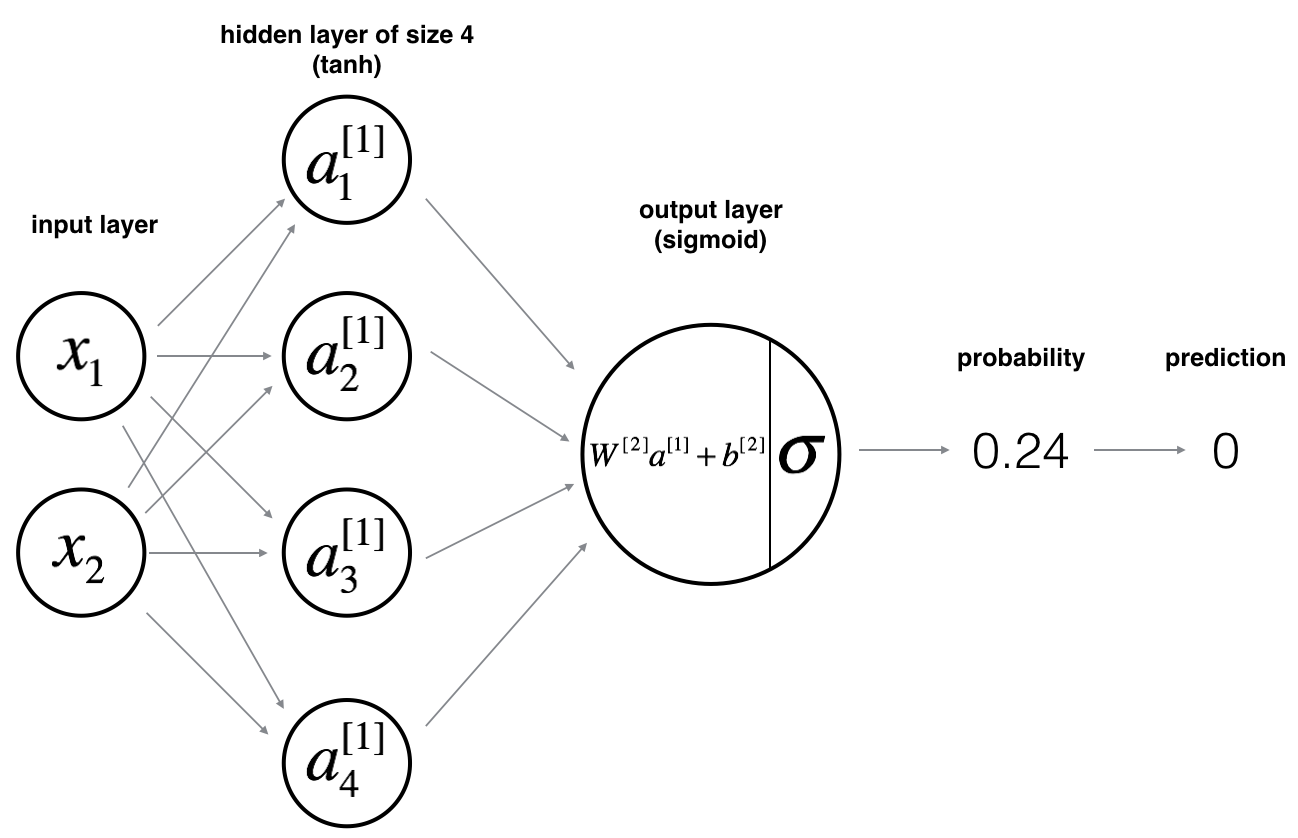
\includegraphics[width=12cm]{classification_kiank.png}
    \caption{An example of an 1-hidden layer neural network}
    \label{fig:classification}
    \end{figure}
\item
For a single training example $x \rightarrow a^{[2]} = \hat{y}$
    \begin{align*}
    z^{[1]} & = W^{[1]}a^{[0]} + b^{[1]}\\
    a^{[1]} &= \sigma(z^{[1]})\\   
    z^{[2]} & = W^{[2]}a^{[1]} + b^{[2]}\\
    a^{[2]} &= \sigma(z^{[2]})
    \end{align*}
\item
Vectorizing across multiple examples
    \begin{align*}
    a^{[l](i)} &: l - \text{layer}; i - \text{example} \ i\\
    X & = \begin{bmatrix} |&|& &| \\ x^{(1)} & x^{(2)} & \cdots & x^{(m)} \\ |&|& &| \end{bmatrix} \in \mathbb{R}^{n_x \times m}\\
    Z & = \begin{bmatrix} |&|& &| \\ z^{[1](1)} & z^{[1](2)} & \cdots & z^{[1](m)} \\ |&|& &| \end{bmatrix} \in \mathbb{R}^{\#\text{(hidden units)} \times m}\\
     A & = \begin{bmatrix} |&|& &| \\ a^{[1](1)} & a^{[1](2)} & \cdots & a^{[1](m)} \\ |&|& &| \end{bmatrix} \in \mathbb{R}^{\#\text{(hidden units)} \times m}\\
     Z^{[1]} &= W^{[1]}X + b^{[1]}\\
     A^{[1]} &= \sigma(Z^{[1]})\\
     Z^{[2]} &= W^{[2]}A^{[1]}+ b^{[2]}\\
     A^{[2]} &= \sigma(Z^{[2]})
    \end{align*}
\end{itemize}

%
\subsection{Activation functions}
\begin{enumerate}
\item
$a = g(z) = \frac{1}{1+e^{-z}}$, sigmoid (except for the output layer of binary classification)\\
$g'(z) = \diff{g(z)}{z} = g(z)(1-g(z)) = a(1-a)$
\item
$a=g(z) = \tanh(z) = \frac{e^z - e^{-z}}{e^z + e^{-z}}$\\
$g'(z) = \diff{g(z)}{z} = 1 - (\tanh(z))^2 = 1-a^2$\\
\item
$g(z)=\max{(0, z)}$, ReLU, rectified linear unit\\
\begin{equation}
g'(z) = \left\{ 
    \begin{array}{rll}
    0 & \text{if} & z < 0 \\
    1 & \text{if} & z > 0 \\
    \text{undefined} & \text{if} & z = 0
    \end{array} \right.
\end{equation}
\item
$a = \max{(0.01z, z)}$, leaky ReLU\\
\begin{equation}
g'(z) = \left\{ 
    \begin{array}{rll}
    0.01 & \text{if} & z < 0 \\
    1 & \text{if} & z > 0 \\
    \text{undefined} & \text{if} & z = 0
    \end{array} \right.
\end{equation}
\end{enumerate}

%
\subsection{Backpropagation}

Forward propagation
\begin{align*}
Z^{[1]} &= W^{[1]}X + b^{[1]}\\
A^{[1]} &= g(Z^{[1]})\\
Z^{[2]} &= W^{[2]}A^{[1]}+ b^{[2]}\\
A^{[2]} &= \sigma(Z^{[2]})
\end{align*}
\\
Backpropagation
\begin{align*}
dZ^{[2]}  &= A^{[2]} -Y\\
dW^{[2]} &= \frac{1}{m}dZ^{[2]}A^{[1]T}\\
db^{[2]}  &= \frac{1}{m}np.sum(dZ^{[2]}, axis = 1, keepdims = True)\\
dZ^{[1]}  &= W^{[2]T}dZ^{[2]}*g^{[1]'}(Z^{[1]})\\
dW^{[1]} &= \frac{1}{m}dZ^{[1]}X^{T}\\
db^{[1]}  &= \frac{1}{m}np.sum(dZ^{[1]}, axis = 1, keepdims = True)
\end{align*}

\emph{\textcolor{Bittersweet}{Initialize the weights randomly, e.g., $W^{[1]} = np.random.randn((2,2))*0.01, b^{[1]} = np.zeros((2,1))$, $\tanh$ or sigmoid activation function usually prefers very small weights (large weights $\rightarrow$ large inputs $\rightarrow$ 0 gradients). All zeros initialization leads to the symmetry breaking problem. In general, initializaing all the wights to zero results in the network failing to break symmetry. This means that every neuron in each layer will the the same thing, this way, the network is no more powerful than a linear classifier like logistic regression.}}


%_________________________________________________________________
\section{Deep L-layer Neural Network}
\label{sec:LNN}

``shallow'' vs. ``deep''\\
logistic regression $\rightarrow$ 1 hidden layer $\rightarrow$ 2 hidden layers $\rightarrow$ L hidden layers
\begin{figure}[h]
    \centering
    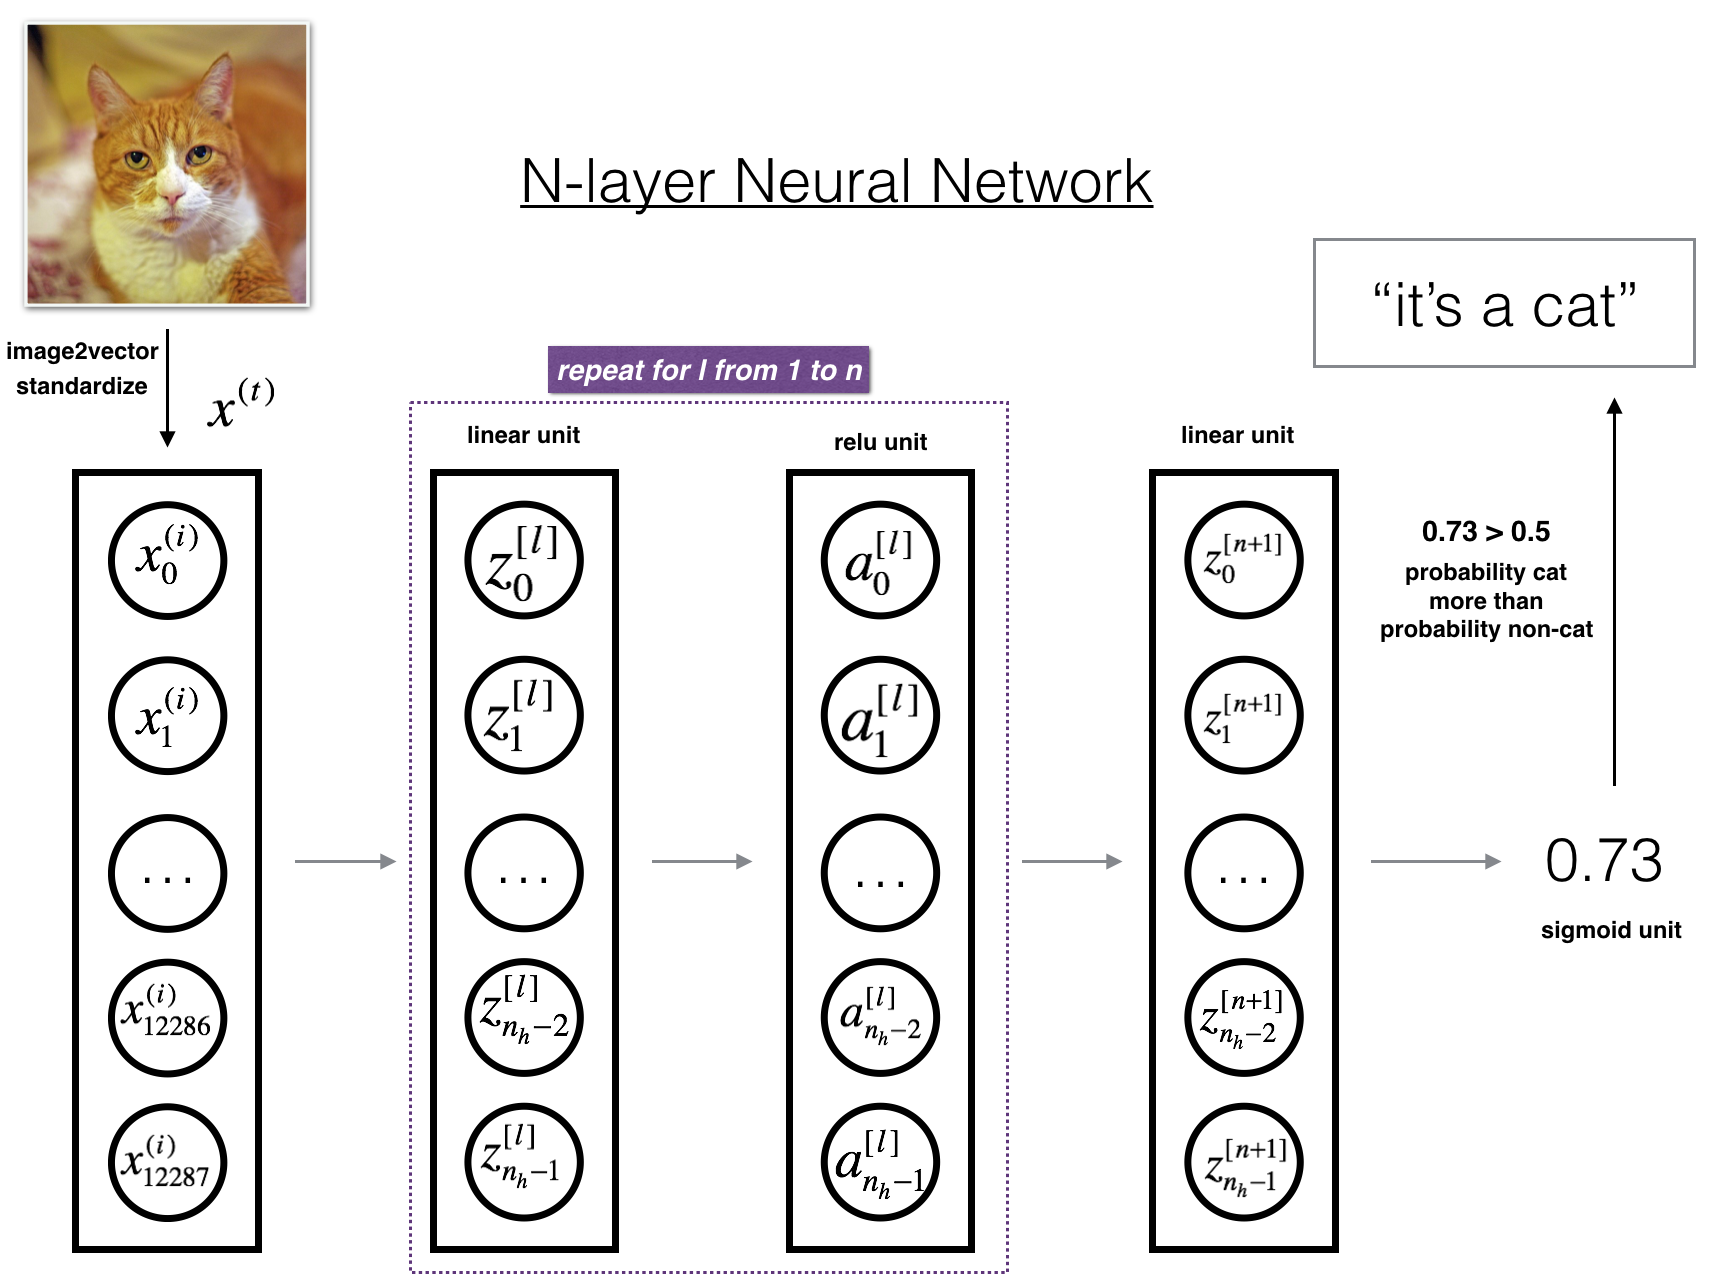
\includegraphics[width=14cm]{NlayerNN.png}
    \caption{An example of an N-layer Neural Network: (LINEAR $\rightarrow$ RELU)  $\times$ (L-1) $\rightarrow$ LINEAR$\rightarrow$ SIGMOID}
    \label{fig:NlayerNN}
\end{figure}

%
\subsection{Notation}
\begin{itemize}
\item
$l$: \# of layers
\item
$n^{[l]}$: \# of units in layer $l$, $n^{[0]} = n_x$.
\item
$a^{[l]}$: activations in layer $l$, $a^{[l]} = g^{[l]}(z^{[l]})$.\\
$w^{[l]}, b^{[l]}$: weights and bias for computing $z^{[l]}$.
\item
$x = a^{[0]}, \hat{y} = a^{[L]}$.
\end{itemize}

%
\subsection{Forward propagation in a deep network}
for a single training example:
\begin{align}
z^{[l]} &= W^{[l]}a^{[l-1]} + b^{[l]}\\
a^{[l]} &= g^{[l]}(z^{[l]})
\end{align}
\\
dimensions of the matrices:
\begin{align*}
W^{[l]}, dW^{[l]}&: (n^{[l]}, n^{[l-1]})\\
b^{[l]}, db^{[l]} &: (n^{[l]}, 1)\\
z{[l]}, a{[l]} &: (n^{[l]}, 1)\\
x, a^{[0]}&: (n^{[0]}, 1)
\end{align*}
\\
vectorized for the whole training set (the training examples stacked in different columns):
\begin{align}
Z^{[l]} &= W^{[l]}A^{[l-1]} + b^{[l]}\\
A^{[l]} &= g^{[l]}(Z^{[l]})
\end{align}
\\
dimensions of the matrices:
\begin{align*}
Z{[l]}, A{[l]}&: (n^{[l]}, m)\\
dZ{[l]}, dA{[l]}&: (n^{[l]}, m)\\
X, A^{[0]}&: (n^{[0]}, m)\\
W^{[l]}, dW^{[l]}&: (n^{[l]}, n^{[l-1]})\\
b^{[l]}, db^{[l]} &: (n^{[l]}, 1), \text{broadcast to}  (n^{[l]}, m)
\end{align*}

%
\subsection{Backpropagation in a deep network}
Forward and backward functions
% Insert the figure here
\begin{figure}[h]
    \centering
    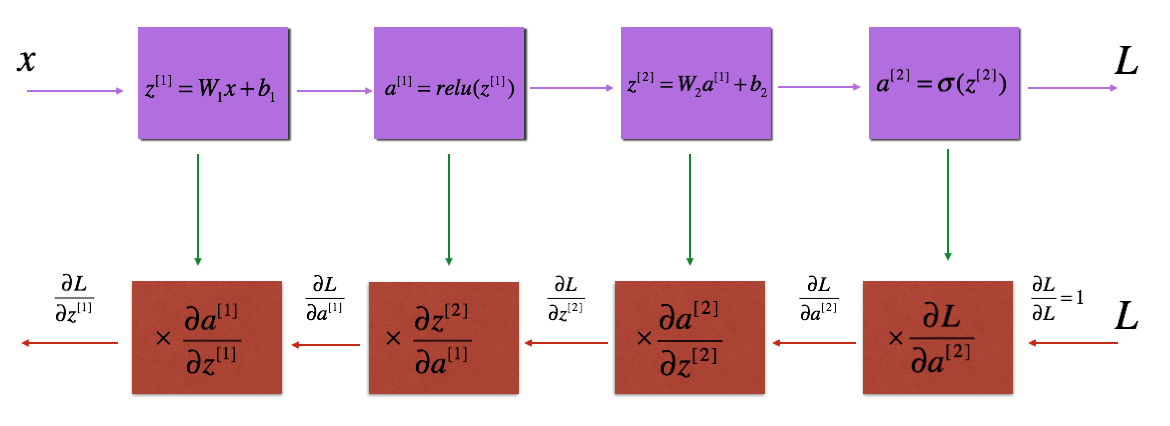
\includegraphics[width=16cm]{ForwardBackwardFuncs.png}
    \caption{Basic blocks of forward and backward functions: $\frac{\partial L}{\partial {W_1}} = \frac{\partial L}{\partial  {a^{[2]}}} \frac{\partial{a^{[2]}}}{\partial  {z^{[2]}}} \frac{\partial{z^{[2]}}}{\partial  {a^{[1]}}} \frac{\partial{a^{[1]}}}{\partial {W_1}}$}
    \label{fig:ForwardBackwardFuncs}
    \end{figure}
\\
Backpropagation
\begin{align}
dZ^{[L]} &= A^{[L]} - Y\\
dW^{[L]} &=  \frac{1}{m}dZ^{[L]}A^{[L-1]T}\\
db^{[L]} &= \frac{1}{m}np.sum(dZ^{[L]}, axis = 1, keepdims = True)\\
dZ^{[L-1]} &= W^{[L]T}dZ^{[L]} * g^{'[L-1]}(Z^{[L-1]})\\
dZ^{[l]} &= dA^{[l]} * g^{'[l]}(Z^{[l]})\\
dW^{[l]} &= \frac{1}{m}dZ^{[l]}A^{[l-1]T}\\
db^{[l]} &= \frac{1}{m}np.sum(dZ^{[l]}, axis = 1, keepdims = True)\\
dA^{[l-1]} &= W^{[l]T}dZ^{[l]}
\end{align}
Note that $*$ denotes element-wise multiplication\footnote{For the cross-entropy cost $J = -\frac{1}{m}(y^{(i)}\log{(a^{[L](i)})} + (1-y^{(i)}\log{(a^{[L](i)})}))$, the gradient $dA^{L} = \diff{J}{A^{{L}}}$ is dAL = - (np.divide(Y, AL) - np.divide(1 - Y, 1 - AL))}.

%
\subsection{Hyperparameters}
\begin{itemize}
\item
learning rate $\alpha$
\item
\# iterations
\item
\# hidden layer $L$
\item
\# hidden units $n^{[1]}, n^{[2]}, \cdots n^{[L]}$
\item
choice of activation function
\item
momentum, minibatch size, regulations, $\cdots$
\end{itemize}
\emph{\textcolor{Bittersweet}{Applied deep learning is a very empirical/iterative process (keep trying a lot of things and see what works): Idea $\rightarrow$ Code $\rightarrow$ Experiment; Cost $J$ vs. \# of iterations. Just have to try out many different values and go around the cycle.}}


%_________________________________________________________________
\section{Applied ML}
\label{sec:AppliedML}

\begin{itemize}
\item
    Train/dev/test sets\\
    Data $\rightarrow$ Training set;``Dev'' (Hold-out cross validation, development set); Test\\
    Big data example: 98/1/1\%; 99.5/0.4/0.1\%\\
    Mismatched train/test distribution: make sure that the dev and test come from the same distribution. Not having a test set might be okay, i.e., only dev set. ``train/dev'' vs. ``train/test''.
\item
    Bias / Variance
    \begin{itemize}
    \item
    Train set error
    \item
    Dev set error
    \end{itemize}    
    \begin{center}
    \begin{tabular}{| m{3cm} | m{2.5cm} | m{2cm} | m{2.5cm} | m{2.5cm} | }
    \hline
    Train set error: & 1\%   & 15\% & 15\% & 0.5\%\\
    Dev set error:   & 11\% & 16\% & 30\% & 1\%\\
    			    & high variance & high bias &  high variance, high bias & low variance, low bias\\
    \hline
    \end{tabular}
    \end{center}
    \emph{High bias}? (training data performance) $\rightarrow$ \emph{Bigger network}; Train longer; advanced optimization algorithms; NN architecture search.\\
    \emph{High variance}? (dev set performance) $\rightarrow$ \emph{More data}; Regularization; NN architecture search\\
    \indent $\rightarrow$ Low bias and low variance.
\end{itemize}

%
\subsection{Regularization}
    
%%
\subsubsection{Logistic regression}
\begin{align}
J(w,b) &= \frac{1}{m}\sum_{i = 1}^{m}L(\hat{y}^{(i)}, y^{(i)}) + \frac{\lambda}{2m}\|w\|_2^2\\
\text{L2 regularization}&: \|w\|_2^2 = \sum_{j = 1}^{n_x}w_j^2 = w^Tw\\
\text{L1 regularization}&: \frac{\lambda}{2m}\sum_{j = 1}^{n_x}|w_j| = \frac{\lambda}{2m}\|w\|_1
\end{align}
$\lambda = $ regularization parameters, which is usually set with the development set (cross validation).\\
L1 regularization makes the model sparse, which is not very helpful for the purpose of compressing the model.\\

%%
\subsubsection{Neural networks}
\begin{align}
J(W^{[1]}, b^{[1]}, \cdots, W^{[L]}, b^{[L]}) &= \frac{1}{m}\sum_{i = 1}^{m}L(\hat{y}^{(i)}, y^{(i)}) + \frac{\lambda}{2m}\sum_{l=1}^{L}\|W^{[l]}\|_F^2\\
\text{Frobenius norm}&: \| W^{[l]} \|_F^2 = \sum_{i = 1}^{n^{[l]}}\sum_{j = 1}^{n^{[l-1]}}(W_{i,j}^{[l]})^2
\end{align}
``Weight decay'': 
\begin{align*}
dW^{[l]} &=  \frac{1}{m}dZ^{[l]}A^{[l-1]T}+ \frac{\lambda}{m}W^{[l]}\\
W^{[l]} :&= W^{[l]} -\alpha dW^{[l]}\\
	&=W^{[l]} -\alpha  (\frac{1}{m}dZ^{[l]}A^{[l-1]T} + \frac{\lambda}{m}W^{[l]})\\
	&=(1-\frac{\alpha \lambda}{m})W^{[l]} -\alpha ( \frac{1}{m}dZ^{[l]}A^{[l-1]T})
\end{align*}
The regularization term penalizes the weight being too large. With ``weight decay'', weights are pushed to smaller values.


%%
\subsubsection{Dropout regularization}

Randomly knocking out units in the network: To go through each of the layers of the network and set some probability of eliminating a node in neural network. For each training example, train it using one of such smaller diminished networks. Dropout is only used during training (applied to both forward and backward propagation), NOT during test time.\\\\
Implementation ``Inverted dropout''.\\
\underline{Example}: Illustrate with layer $l = 3$, 
\begin{lstlisting}[language=Python]
keep_prob = 0.8
d3 = np.random.rand(a3.shape[0], a3.shape[1]) < keep_prob
a3 = np.multiply(a3, d3) # a3*= d3
a3 /= keep_prob # in order to not reduce the expected value of z4
\end{lstlisting}
Intuition: Can't rely on any one feature, so have to spread out weights $\rightarrow$ shrinking the weights, similar effect as to L2 regularization (an adaptive form of L2 regularization).
\\\\
Downside: the cost function $J$ is no longer well defined.

%%
\subsubsection{Other regularization methods}
\begin{itemize}
\item
Data augmentation, e.g., flipping horizontally, taking random crops/rotations/distortions/translations of the pictures to create additional fake training examples.
\item
Early stopping\\
Plot the training error vs. \# iterations and the dev set erorr vs. \# iterations, stop half way to get mid-size $\|w\|_F^2$\\
Downside: the tasks of optimizing cost function and reducing variance are no long orthogonalized (c.f., L2 regularization with trying out a lot of values of the hyperparameter $\lambda$).
\end{itemize}


%
\subsection{The optimization problem}

%%
\subsubsection{Normalizing training sets}
(Rough intuition: the cost function will be faster and easier to optimize when the features are on similar scales).\\
Subtract mean and normalize variance:
\begin{align*}
\mu &= \frac{1}{m}\sum_{i = 1}^{m}x^{(i)}, \quad
\sigma^2= \frac{1}{m}\sum_{i = 1}^{m}(x^{(i)} - \mu)^2\\
x^{(i)} &:= \frac{x^{(i)} - \mu}{\sigma}
\end{align*}
Use the same $\mu, \sigma^2$ to normalize the test set.

%%
\subsubsection{Vanishing/Exploding gradients}
Activation/gradients increase/decrease exponentially as a function of the number of layers.\\\\
$n \rightarrow$ careful choice of the random initialization of the neural network.\\\\
large $n \rightarrow$ smaller $w$\\
$W^{[l]} = np.random.randn(shape)*np.sqrt(\frac{2}{n^{[l-1]}})$
\\\\
ReLU: $Var(w) = \sqrt{\frac{2}{n^{[l-1]}}}$, He initialization\\
$\tanh: Var(w) = \sqrt{\frac{1}{n^{[l-1]}}}$, Xavier initialization\\
$Var(w) = \sqrt{\frac{2}{n^{[l-1]} * n^{[l]}}}$\\


%%
\subsubsection{Gradient checking}
Numerical approximation of gradients
\begin{align*}
\frac{f(\theta +\epsilon) - f(\theta -\epsilon)}{2\epsilon} \approx g(\theta)
\end{align*}
\\
Take all the $W^{[1]}, b^{[1]}, \cdots, W^{[L]}, b^{[L]}$ and reshape into a big vector $\theta$.\\
Take all the $dW^{[1]}, db^{[1]}, \cdots, dW^{[L]}, db^{[L]}$ and reshape into a big vector $d\theta$.\\
Is $d\theta$ the gradients of $J(\theta)$?\\\\
for each $i$:\\
\indent $d\theta_{\text{approx}}[i] = \frac{J(\theta_1, \theta_2, \cdots, \theta_i + \epsilon, \cdots) - J(\theta_1, \theta_2, \cdots, \theta_i - \epsilon, \cdots) }{2\epsilon}$\\
check, e.g., $\frac{\|d\theta_{\text{approx}} - d\theta\|_2}{\|d\theta_{\text{approx}}\|_2 +\|d\theta\|_2} \approx 10^{-7} \text{when} \ \epsilon \approx 10^{-7}$
\begin{itemize}
\item
Don't use in training -- only to debug.
\item
If algorithm fails the gradient checking, look at components to try to identify bug.
\item
Remember regularization.\\
$J(\theta)$ includes the regularization term.
\item
Doesn't work with dropout.
\item
Run at random initialization; perhaps again after training.
\end{itemize}


%_________________________________________________________________
\section{Optimization algorithms}
\label{sec:Optimization}

%
\subsection{Mini-batch gradient descent}
mini-batch: split the training data into smaller training sets, $X^{\{t\}}, Y^{\{t\}} \in \mathbb{R}^{n_x \times \frac{m}{n_\text{mini-batch}}}$\\
``1 epoch (a single pass through a mini-batch)'': Forward propagation, compute the $J^{\{t\}}$ using $X^{\{t\}}, Y^{\{t\}}$, and update the parameters with backprob accordingly on each mini-batch.
\\\\
Choosing the mini-batch size:
\begin{itemize}
\item
If mini-batch size = m: Batch gradient descent $\rightarrow$ too long per iteration
\item
If mini-batch size = 1: Stochastic gradient descent $\rightarrow$ lose speedup from vectorization

    \begin{itemize}
    \item
    If small training set: Use batch gradient descent ($m \leq 2000$)
    \item
    Typical mini-batch size: 64, 128, 256, 512, 1024
    \item
    Make sure that all the minibatch fit in CPU/GPU memory
    \item
    Tune as another hyperparameter
    \end{itemize}
\end{itemize}

\begin{figure}[h]
    \centering
    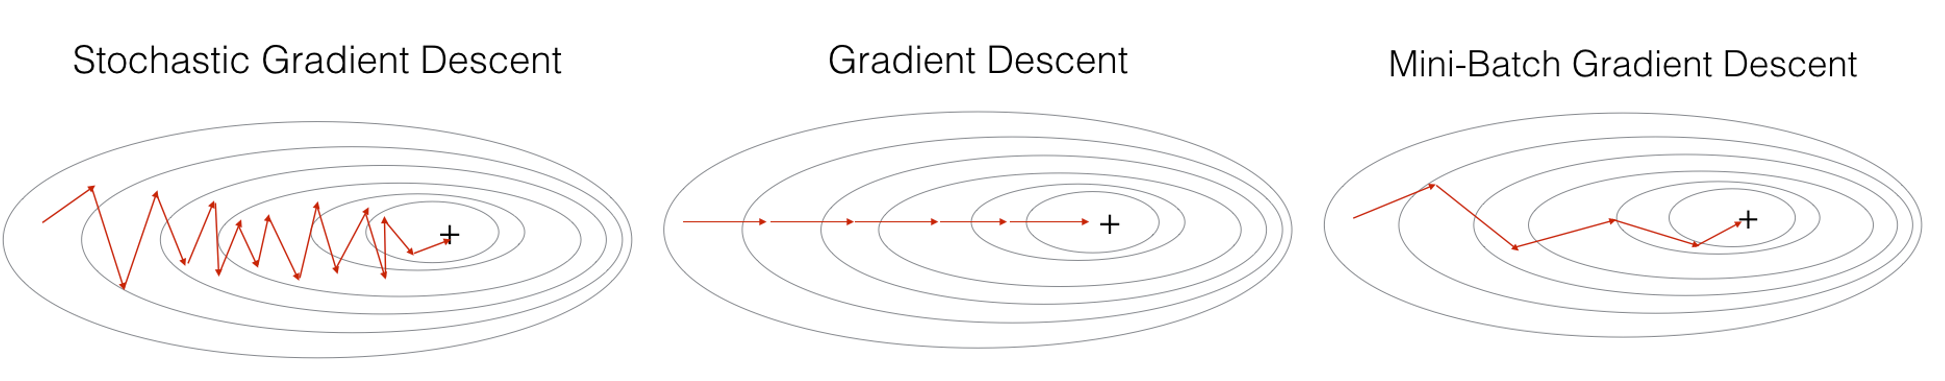
\includegraphics[width=16cm]{descent.png}
    \caption{Comparison of different gradient descent methods}
    \label{fig:descent}
\end{figure}

%
\subsection{Exponentially weighted (moving) averages}
$v_t = \beta v_{t-1} + (1-\beta)\theta_t$\\
rule of thumb: $(1-\epsilon)^{\frac{1}{\epsilon}} = \frac{1}{e}$\\
e.g., $0.9^{10} \approx 0.35 \approx \frac{1}{e}$\\
e.g., $0.98^{50} \approx \frac{1}{e}$\\
\\
$v_{\theta} = 0$\\
Repeat\{\\
\indent Get next $\theta_t$\\
\indent $v_{\theta} := \beta v_{\theta} + (1-\beta)\theta_t$\\
\}
\\
Bias correction: $\displaystyle\frac{v_t}{1-\beta_t}$\\
\\
damping out the oscillations in gradient descent and allowing the use of a larger learning rate to speed up the learning speed of the algorithm.

%
\subsection{Gradient descent with momentum}
\textbf{Momentum}\\
Momentum takes past gradients into account to smooth out the steps of gradient descent.
\\
On iteration t:\\
\indent Compute $dw, db$ on current mini-batch.\\
\indent $\displaystyle v_{dW} = \beta v_{dW} + (1-\beta)dW$\\
\indent $\displaystyle v_{db} = \beta v_{db} + (1-\beta)db$\\
\indent $\displaystyle W := W-\alpha v_{dW}, b := b - \alpha v_{db}$\\
Hyperparmeters: $\alpha, \beta$, e.g., $\beta = 0.9$, average over about the 10 gradients.\\
The larger the mementum $\beta$ is, the smoother the update, because it takes the past gradients into account more. But if $\beta$ is too big, it could also smooth out the updates too much. Common values for $\beta$ range from 0.8 to 0.999. Turing the optimal $\beta$ might require several values to see what works best in terms of reducing the cost function $J$.


%
\subsection{RMSprop}
\textbf{Root mean square prop}
\\
An exponentially weighted average of the squares of the past gradients, second moment estimates.
\\
On iteration t:
\\
\indent Compute $dw, db$ on current mini-batch.\\\\
\indent $\displaystyle s_{dW} = \beta_2 s_{dW} + (1-\beta_2)dW^2$ (element-wise squre)\\\\
\indent $\displaystyle s_{db} = \beta_2 s_{db} + (1-\beta_2)db^2$ \\\\
\indent $\displaystyle W := W-\alpha \frac{dW}{\sqrt{s_{dW}}+\epsilon}, b = b - \alpha \frac{db}{\sqrt{s_{db}}+\epsilon}$, e.g., $\epsilon = 10^{-8}$ numerical stability.

%
\subsection{Adam optimization algorithm}
\textbf{Adam: Adaptive moment estimation}
\\
$s_{dW} = 0, s_{dW} = 0, v_{db} = 0, s_{db} = 0$\\
On iteration t:\\
\indent Compute $dw, db$ on current mini-batch.\\
\\
\indent $\displaystyle v_{dW} = \beta_1 v_{dW} + (1-\beta_1)dW$,
            $\displaystyle v_{db} = \beta_1 v_{db} + (1-\beta_1)db$\\\\
\indent $\displaystyle s_{dW} = \beta_2 s_{dW} + (1-\beta_2)dW^2$,
            $\displaystyle s_{db} = \beta_2 s_{db} + (1-\beta_2)db^2$ \\\\
\indent $\displaystyle v_{dW}^{\text{corrected}} = v_{dW}/(1-\beta^t_1),
                v_{db}^{\text{corrected}} = v_{db}/(1-\beta^t_1)$\\\\
\indent $\displaystyle s_{dW}^{\text{corrected}} = s_{dW}/(1-\beta^t_2),
                s_{db}^{\text{corrected}} = s_{db}/(1-\beta^t_2)$\\\\
\indent $\displaystyle W := W-\alpha \frac{v_{dW}^{\text{corrected}}}{\sqrt{s_{dW}^{\text{corrected}} }+\epsilon},
                b = b - \alpha \frac{v_{db}^{\text{corrected}}}{\sqrt{s_{db}^{\text{corrected}}}+\epsilon}$\\
\\
Hyperparameters choice:\\
$\alpha$: needs to be tuned\\
$\beta_1: 0.9$\\
$\beta_2: 0.999$\\
$\epsilon: 10^{-8}$

%
\subsection{Learning rate decay}
1 epoch: 1 pass through the whole training data\\\\
$\displaystyle \alpha = \frac{1}{1 + \text{decayRate} \times \text{epochNumber}} \alpha_0$\\
\\
Other learning rate decay methods:\\\\
$\displaystyle \alpha = 0.95^{\text{epochNumber}} \alpha_0$\\
$\displaystyle \alpha = \frac{k}{\text{epochNumber}} \alpha_0$ or $\alpha = \frac{k}{t} \alpha_0$\\
$\displaystyle \alpha = \frac{1}{1 + \text{decayRate} \times \lfloor\frac{\text{epochNumber}}{\text{timeInterval}}\rfloor} \alpha_0$\\\\
manual decay, etc.


%_________________________________________________________________
\section{Improving deep neural networks}

%
\subsection{Hyperparameter tuning}
\begin{itemize}
\item
Hyperparameters: $\alpha, \beta, \beta_1, \beta_2, \epsilon$, \# layers, \#hidden units, learning rate dacay, mini-batch size\\
Sampling randomly rather than using a grid, coarse to fine search process.
\item
Using an appropriate scale to pick hyperparameter:\\
Using the log scale instead of a linear scale.
\begin{align*}
r & \in [\log_{10}0.0001, \log_{10}1] = [-4, 0]\\
\alpha & = 10^r
\end{align*}
Hyperparameters for exponentially weighted averages:\\
$\beta = 0.9, \cdots, 0.999$\\
sampling $1 -\beta$ instead of $\beta$ using the log scale.
\item
Hyperparameters tuning in practice: babysitting one model vs. training many models in parllel.\\
\end{itemize}

%
\subsection{Normalizing activations in a netowrk}
Can we normalize $a^{[l]}$ so as to train $w^{[l+1]}, b^{[l+1]}$ faster?\\
Implementing batch norm:\\
Given some intermediate values in NN $z^{[l](i)}$,
\begin{align*}
\mu &= \frac{1}{m}\sum_{i = 1}^{m}z^{[l](i)}\\
\sigma^2 & = \frac{1}{m}\sum_{i = 1}^{m}(z^{[l](i)} - \mu)^2\\
z^{[l](i)}_{\text{norm}} &= \frac{z^{[l](i)} - \mu}{\sigma + \epsilon}\\
\tilde{z}^{[l](i)} &= \gamma z^{[l](i)}_{\text{norm}} + \beta
\end{align*}
$\gamma, \beta$ are learnable parmeters of the model (avoiding the hidden units to always have mean 0 and variance 1), e.g., if $\gamma = \sigma + \epsilon, \beta = \mu$, then $\tilde{z}^{[l](i)} = z^{[l](i)}_{\text{norm}}$.\\
\\
\textbf{Working with mini-batches}\\

$ X^{\{t\}} \xrightarrow[ ]{w^{[1]}} Z^{[1]} \xrightarrow[\text{BN}]{\beta^{[1]}, \gamma^{[1]}} \tilde{Z}^{[1]}  \rightarrow a^{[1]} = g^{[1]}(\tilde{Z}^{[1]}) \xrightarrow[]{w^{[2]}} Z^{[2]} \xrightarrow[\text{BN}]{\beta^{[2]}, \gamma^{[2]}} \tilde{Z}^{[2]}  \rightarrow a^{[2]} = g^{[2]}(\tilde{Z}^{[2]}) \xrightarrow[ ]{\cdots} \cdots$\\
\begin{enumerate}
\item
``covariates shift''\\
It limits the amoun to which updating the parameters in the earlier layers can affect the distribution of values that the later layers have to learn on. It reduces the problem of the input values changing (stablize). It weakens the coupling between between the parameters of earlier and later layers.
\item
``regularization effect''\\
Each mini-batch is scaled by the mean/variance computed on just that mini-batch, which adds some noise to the values $z^{[l]}$ within that minimatch. So similar to dropout, it adds some noise to each hidden layer's activation. A bigger batch size will reduce the noise. But batch norm is not supposed to be used as regularization.
\end{enumerate}
\textbf{Working with testing set}\\
$\mu, \sigma^2$: estimate using exponentially weighted average (across mini-batch).
\begin{align*}
X^{1} &\rightarrow \mu^{\{1\}[l]}\\
X^{2} &\rightarrow \mu^{\{2\}[l]}\\
X^{3} &\rightarrow \mu^{\{3\}[l]}\\
&\vdots\\
&\rightarrow\\
&\mu (\text{exponentially weighted average})
\end{align*}

\emph{\textcolor{Bittersweet}{If you are going to fine-tune a pretrained model, it is important that you block the weights of all your batchnormalization layers.}}

%
\subsection{Multi-class classification: Softmax regression}
\begin{align}
z^{[l]} &= W^{[l]}a^{[l-1]} + b^{[l]} \nonumber \\
t &= e^{(z^{[l]})} (\text{element-wise exponentiation})\\
a^{[l]} &= g^{[l]}(z^{[l]}) = \frac{t_i}{\sum_{i = 1}^C t_i}
\end{align}
When $C = 2$, the softmax reduces to the logistic regression.
%%
\subsubsection{Loss function}
\begin{align}
L(\hat{y},y) &= -\sum_{j= 1}^C y_j \log{\hat{y}_j}\\
J(w, b, \cdots)&= \frac{1}{m}\sum_{i= 1}^m L(\hat{y}^{(i)},y^{(i)})\\
&\text{(maximum likelihood estimation)}
\end{align}
\\
\textbf{Gradient descent with softmax}
$$\frac{\partial J}{\partial z^{[L]}} = \hat{y} - y$$


%_________________________________________________________________
\section{ML strategy}
Collect more data;
Collect more diverse training set;
Train algorithm long with gradient descent;
Try Adam instead of gradient descent;
Try bigger network;
Try smaller network;
Try dropout;
Add $L_2$ regularization;
Network architecture (activation function, \#hidden layers, $\cdots$);
$\cdots$

%
\subsection{Orthogonalization}
What to tune in order to achieve one effect.\\
Chain of assumptions in ML:
\begin{itemize}
\item[]
Fit training set well on cost function: Bigger network, Adam, etc.
\item[]
Fit dev set well on cost function: Regularization, etc.
\item[]
Fit test set well on cost function: Bigger dev set, etc.
\item[]
Performs well in real world: Change the dev set or the cost function, etc.
\end{itemize}
Orthogonalized controls make the process of tuning the network easier.\\
\\
\textbf{Single number evaluation metric}\\
Satisficing and optimizing metric\\
N matices: 1 optimizing and N-1 satisficing.\\

%
\subsection{Train/Dev/Test distributions}
Taget: Dev set + metric.\\
Make sure that the dev set and the test set come from the same distribution.\\
$\rightarrow$ Randomly shuffle the data into dev/test.\\
Choose a dev set and test set to reflect data you expect to get in the future and consider important to do well on.\\
\\
98\% training, 1\% dev,  1\% training\\
Size of the test set: Set the test set to be big enough to give high confidence in the overall performance of the system.\\
When to change Dev/test sets and metrics? When the evaluation metric is no longer correctly rank ordering preferences between algorithms. If doing well on the metric + dev/test set does not correspond to doing well on the application, change the metric and/or dev/test set. e.g., $J = \frac{1}{m}\sum_{i = 1}^mL(\hat{y}^{(i)}, y^{(i)}) \rightarrow J = \frac{1}{\sum w^{(i)}}\sum_{i = 1}^m w^{(i)} L(\hat{y}^{(i)}, y^{(i)})$

%
\subsection{Comparing to human-level performance}
Bayes optimal error (best possible error).
Humans are quite good at a lot of tasks. So long as ML is worse than humans, you can:
\begin{itemize}
\item[]
Get labeled data from humans.
\item[]
Gain insight from manual error analysis: Why did a person get this right?
\item[]
Better analysis of bias/varaince.
\end{itemize}
Human-level error as a proxy for Bayes error. Understanding the estimate of Bayes error causes the decisions in choosing what to focus on.
\begin{itemize}
\item
Human level error vs. Training error: ``avoidable bias''\\
$\rightarrow$ Train bigger model; Train longer/better optimization algorithms (e.g., RMSprop, Adam, etc.); NN architecture/hyperparameters search (e.g., RNN, CNN, etc.)
\item
Training error vs. Dev error: ``variance''\\
$\rightarrow$ More data; Regularization (e.g., L2, dropout, data augmentation, etc.); NN architecture/hyperparameters search
\end{itemize}

Problems where ML significantly surpasses human-level performance:
\begin{itemize}
\item[]
Online advertising
\item[]
Product recommendations
\item[]
Logistics (predicting transit time)
\item[]
Loan approvals
\item[]
Speech recognition
\item[]
Some image recognition, medical data, etc.
\end{itemize}
~\\
The two fundatmental assumptions of supervised learning:
\begin{enumerate}
\item
You can fit the training set pretty well
\item
The training set performance generalizes pretty well to the dev/test set
\end{enumerate}


%_________________________________________________________________
\section{Structuring ML projects}
%
\subsection{Error analysis}
Look at dev examples to evaluate ideas\\
Check the ``ceiling'', upper bound on the performance, to evaluate whether or not a single idea is worth working on.\\
Evaluate multiple ideas in parallel.\\
$\rightarrow$ a sense of the best options.

%%
\subsubsection{Cleaning up incorrectly labeled data}
DL algorithms are quite robust to random errors in the training set (vs. ``systematic errors''). Only if it makes a significant difference to evaluate the algorithms, it might worthwhile fixing the incorrect labels.\\
\underline{Example}:\\
Overall dev set error: 10\%\\
Errors due to incorrect labels: 0.6\%\\
Errors due to other causes: 9.4\%
\begin{itemize}
\item[]
Apply same process to the dev and test sets to make sure they continue to come from the same distribution.
\item[]
Consider examining examples the algorithm got right as well as ones it got wrong.
\item[]
Train and dev/test data may now come from slightly different distributions. If the training set comes from a slightly different distribution, it might be just fine.
\end{itemize}
\emph{\textcolor{Bittersweet}{Build your first system quickly, then iterate. Set up dev/test and metric; Build initial system quickly; Use vias/variance analysis and error analysis to prioritize next steps.}}

%
\subsection{Training and testing on different distributions}
\underline{Example}: Training set: 200,000; Test set: 10,000. $\rightarrow$ Training: 20,500; Dev 2,500; Test 2,500.\\
\\
\underline{Example}: Training set: 500,000; Test set: 20,000.

$\rightarrow$ Training: 500,000; Dev 10,000; Test 10,000.

$\rightarrow$ Training: 510,000; Dev 5,000; Test 5,000.\\

\subsubsection{Bias and variance with mismatched data distributions}
Training-dev set: Same distribution as training set, but not used for training.

\begin{center}
\begin{tabular}{| m{4cm} | m{3cm} | m{5cm} | }
\hline
Human error: & 4\% &\\
\hline
Training set error: &7\% & $\rightarrow$ avoidable bias \\
\hline
Training-dev set error: & 10\% & $\rightarrow$ vairance \\
\hline
Dev set error: & 12\% & $\rightarrow$ data mismatch \\
\hline
Test error: &12\% & $\rightarrow$ degree of overfitting \\
\hline
\end{tabular}
\end{center}
~\\
Addressing data mismatch
\begin{itemize}
\item
Carry out manual error analysis to try to understand difference tween training and dev/test sets.
\item
Making the training data more similar; or collect more data similar to dev/test sets.
\end{itemize}
\emph{\textcolor{Bittersweet}{If artificial synthesis data are used, be cautious and bear in mind whether or not you might be accidentally simulating data only from a tiny subset of the space of all possible examples.}}

%
\subsection{Learning from multiple tasks}
\subsection{Transfer learning}
Take knowledge the neural network has learned from one task and apply that knowledge to a separate task (sequential).\\
Having trained the neural network, to implement transfer learning: Swap in a new data set, replace the last output layer with a set of randomly initialized weights for the laster layer and have that output for the new task.\\
\\
``pre-training'' vs. ``fine-tuning''\\
Depending on the size of the new dataset, re-train the last or the several later layer of the network.\\
\\
When does transfer learning make sense?
\begin{itemize}
\item
Task A and B have the same input x.
\item
A lot more data for task A than task B.
\item
Low level features from task A could be helpful for learning B.
\end{itemize}

%
\subsection{Multi-task learning}
start off simultaneously, trying to have one neural network do several things at the same time.\\
\underline{Example}:\\
For $x^{(i)}, \hat{y}^{(i)} \in \mathbb{R}^{4 \times 1}$,\\
$\displaystyle\frac{1}{m}\sum_{i=1}^{m}\sum_{j=1}^{4}L(\hat{y_{j}}^{(i)}, {y_{j}}^{(i)})$, \\sum only over values of $j$ with 0 or 1 label (each object doesn't have to be fully labeled).\\
Instead of training 4 separate neural networks, training one network to do 4 things. If some of the earlier features in the network can be shared between these different types of objects, then training one network to do 4 things results in better performance.\\
\\
Unlike softmax regression, which assigned a single label to single example. Each example has multiple labels. Building a single neural network that is looking at each example and solving multiple problems.\\
\\
When does multi-task learning makes sense?
\begin{itemize}
\item
Training on a set of tasks that could benefit from having shared lower-level features.
\item
Usually: Amount of data you have for each task is quite similar. e.g., 100 task and 1,000 examples per task.
\item
Can train a big enough neural network to do well on all the tasks.
\end{itemize}

%
\subsection{End-to-end deep learning}
Long complicated pipeline (multistep approach) $\rightarrow$ (input-end to output-end) train a huge neural network to just input the raw data and directly output the targets.\\
\\
Speech recognition example\\
audio $\xrightarrow[]{\text{MFCC}}$ features $\xrightarrow[]{\text{ML}}$ Phonemes $\rightarrow$ Words $\rightarrow$  transcript
\\
audio $\xrightarrow{\hspace*{7.6cm}}$ transcript\\
\\
One of the challenges of end-to-end deep learning is that you might need a lot of data before it works well.\\
\\
Pros and Cons of end-to-end deep learning\\

Pros:
\begin{itemize}
\item
Let the data speak.
\item
Less hand-designing of components needed.
\end{itemize}

Cons:
\begin{itemize}
\item
May need large amount of data.
\item
Excludes potentially useful hand-designed components (huge amount of data vs. hand-design)
\end{itemize}
~\\
Applying end-to-end deep learning\\
Key question: Do you have sufficient data to learn a function of the complexity needed to map x to y?



\clearpage
%_________________________________________________________________
\section{Convolutional neural networks}

%
\subsection{Computer vision problem}
Image classification; Object detection; Neural style transfer.\\
Deep learning on large images: enough data to prevent a neural network from overfitting; computational/memory requirements infeasible.\\
In a computer vision application, each value in the matrix corresponds to a single pixel value. A filter is convolved with the image by multiplying its values element-wise with the original matrix, then summing them up and adding a bias.\\
\\
\textbf{``convolution''} operation: filter (kernel) \footnote{``Convolution'' means something different in signal processing or math, cf. cross-correlation.}\\
\underline{Example}: Vertical edge detection:\\
e.g., $\begin{bmatrix}1 & 0 & -1 \\1 & 0 & -1 \\1 & 0 & -1 \end{bmatrix}$\\
Sobel filter:\\
e.g., $\begin{bmatrix}1 & 0 & -1 \\2 & 0 & -2 \\1 & 0 & -1 \end{bmatrix}$\\
Schorr filter:\\
e.g., $\begin{bmatrix}3 & 0 & -3 \\10 & 0 & -10 \\3 & 0 & -3 \end{bmatrix}$\\
\underline{Example}: Horizontal edge detection:\\
e.g., $\begin{bmatrix}1 & 1 & 1 \\0 & 0 & 0 \\-1 & -1 & -1 \end{bmatrix}$\\
\\
Let the numbers in the filter be learned (through backprop) as weights.\\
\\
\textbf{Padding}
\begin{itemize}
\item
It allows you to use a CONV layer without necessarily shrinking the height and width of the volumes. This is important for building deeper networks, since otherwise the height/width would shrink as you go to deeper layers. An important special case is the ``\textbf{same}'' convolution, in which the height/width is exactly preserved after one layer.
\item
It helps us keep more of the information at the border of an image, e.g., zero padding. Without padding, very few values at the next layer would be affected by pixels at the edges of an image.
\end{itemize}

\begin{itemize}
\item
``Valid'' convolution:\\
$(n \times n)  * (f \times f) \rightarrow (n-f+1) \times (n-f+1)$\\
Shrinking output, through away information from edge.
\item
``Same'' convolution:\\
Pad so that output size is the same as the input size
\\
$\rightarrow (n+2p-f+1) \times (n+2p-f+1)$\\
e.g., pad the board with 1 or 2 pixels, $p = \frac{f-1}{2}$\\
$f$ is usually odd.
\end{itemize}
~\\
\textbf{Strided convolution}\\
Stride = amount you move the window each time you slide
padding $p$, stride $s$,\\
$(n \times n)  * (f \times f) \rightarrow \bigfloor{\frac{n+2p-f}{s} + 1} \times \bigfloor{\frac{n+2p-f}{s} + 1}$\\
\\
\textbf{Convolutions over volume}\\
\underline{Example}: Convolutions on RGB images, e.g., hight, width, \#chanels\\
$(6 \times 6 \times 3) * (3 \times 3 \times 3) \rightarrow (4 \times 4)$\\
\\
\textbf{Multiple filters}\\
$n'_c$: \# filters\\
$(n \times n \times n_c) * (f \times f \times n_c) \rightarrow (n-f+1) \times (n-f+1) \times n'_c $

%
\subsection{One layer of a convolutional network}
A convolution layer transforms an input volume into an output volume of different size.\\
\begin{figure}[h]
    \centering
    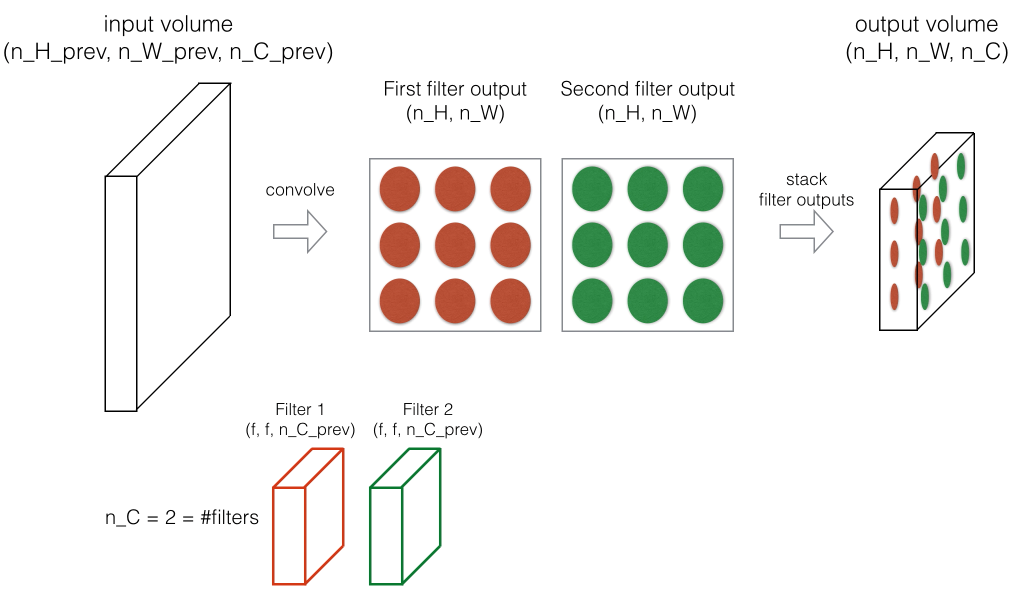
\includegraphics[width=14cm]{convolution.png}
    \caption{Illustration of convolutions}
    \label{fig:convolution}
\end{figure}
Two filters\\
$(6 \times 6 \times 3) * (3 \times 3 \times 3) \rightarrow \text{ReLU}(4 \times 4 + b_1) \rightarrow (4 \times 4)$\\
$\underbrace{(6 \times 6 \times 3)}_{\normalfont a^{[0]}} * \underbrace{(3 \times 3 \times 3)}_{\normalfont w^{[1]}} \rightarrow \text{ReLU}(\underbrace{4 \times 4 + b_2}_{\normalfont z^{[1]}}) \rightarrow (\underbrace{4 \times 4}_{\normalfont a^{[1]}})$\\
$\rightarrow 4 \times 4 \times 2$\\
\\
One property of such a convolution neural network: Less prone to overfitting. Once the feature detectors are learned, they could be applied to larger images and the number of parameters keep fixed (relatively small).\\
\\
If layer $l$ is a convolution layer:\\
$f^{[l]} = $ filter size\\
$p^{[l]} = $ padding\\
$s^{[l]} = $ stride\\
$n_c^{[l]} = $ number of filters\\
Each filter is: $f^{[l]} \times f^{[l]} \times n_c^{[l-1]}$\\
Activations: $a^{[l]} \rightarrow n_H^{[l]} \times n_W^{[l]} \times n_c^{[l]}$\\
Weights: $f^{[l]} \times f^{[l]} \times n_c^{[l-1]} \times n_c^{[l]}$, $n_c^{[l]} $ is the number of filters in layer $l$\\
Bias: $n_c^{[l]} \rightarrow (1,1,1, n_c^{[l]})$\\\\
Input: $(n_H^{[l-1]} \times n_W^{[l-1]} \times n_c^{[l-1]})$\\\\
Output: $(n_H^{[l]} \times n_W^{[l]} \times n_c^{[l]})$\\
\begin{align*}
n_H^{[l]} &= \bigfloor{\frac{n_H^{[l-1]} +2p^{[l]}-f^{[l]}}{s^{[l]}} +1}\\
A^{[l]} &\rightarrow m \times n_H^{[l]} \times n_W^{[l]} \times n_c^{[l]}
\end{align*}

%
\subsection{Simple convolutional network example}
\underline{Example ConvNet}\\\\
$x ~ (39 \times 39 \times 3):$\\
$n_H^{[0]} = n_W^{[0]} = 39, n_c^{[0]} =3$\\
\\
$\longrightarrow$\\
$f^{[1]} = 3, s^{[1]} = 1, p^{[1]} = 0$, 10 filters\\
$n_H^{[1]} = n_W^{[1]} = 37, n_c^{[1]} =10$\\
\\
$a^{[1]} ~ (37 \times 37 \times 10):$\\
\\
$\longrightarrow$\\
$f^{[2]} = 5, s^{[2]} = 2, p^{[2]} = 0$, 20 filters\\
$n_H^{[2]} = n_W^{[2]} = 17, n_c^{[2]} =20$\\
\\
$a^{[2]} ~ (17 \times 17 \times 20):$\\
\\
$\longrightarrow$\\
$f^{[3]} = 5, s^{[3]} = 2, p^{[3]} = 0$, 40 filters\\
$n_H^{[3]} = n_W^{[3]} = 7, n_c^{[3]} =40$\\
\\
$a^{[3]} ~ (7 \times 7 \times 40)$\\
$\longrightarrow$\\
a vector of 1960 (flatten/unroll)\\
$\longrightarrow$\\
logistic regression/softmax
\\
%
\subsection{Types of layers in a convolutional network}
\begin{itemize}
\item
Convolution (CONV)
\item
Pooling (POOL)
\item
Fully connected (FC)
\end{itemize}
~\\
Pooling layer:
Pooling layers gradually reduce the height and width of the input by sliding a 2D window over each specified region, then summarizing the features in that region.
\begin{figure}[h]
    \centering
    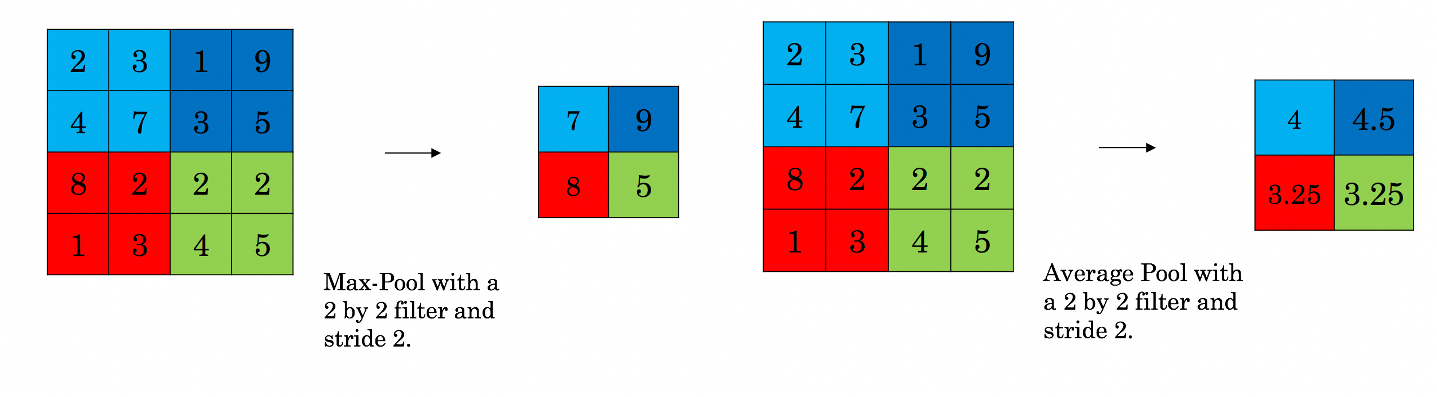
\includegraphics[width=14cm]{pooling.png}
    \caption{Max pooling (left) vs. average pooling (right)}
    \label{fig:pooling}
\end{figure}
\begin{itemize}
\item
Max pooling:\\
slides an $(f, f)$ window over the input and stores the max value of the window in the output.
\item
Average pooling:\\
slides an $(f, f)$ window over the input and stores the average value of the window in the output.
\item
Hyperparameters (f: filter size; s: stride) but no parameters to learn.
\end{itemize}
e.g., $5 \times 5 \xrightarrow[]{f = 3, s =1} 3 \times 3$\\
pooling is applied to each of the channel independently.\\
$n_H \times n_W \times n_c \rightarrow \bigfloor{\frac{n_H - f}{s}+1} \times \bigfloor{\frac{n_H - f}{s}+1} \times n_c $


%
\subsection{CNN Example}

Why convolutions: 
\begin{itemize}
\item
Parameters sharing:\\
A feature detector (such as a vertical edge detector) that's useful in one part of the image is probably useful in another part of the image.
\item
sparsity of connections:\\
In each layer, each output value depends only on a small number of inputs.
\end{itemize}

\begin{figure}[h]
    \centering
    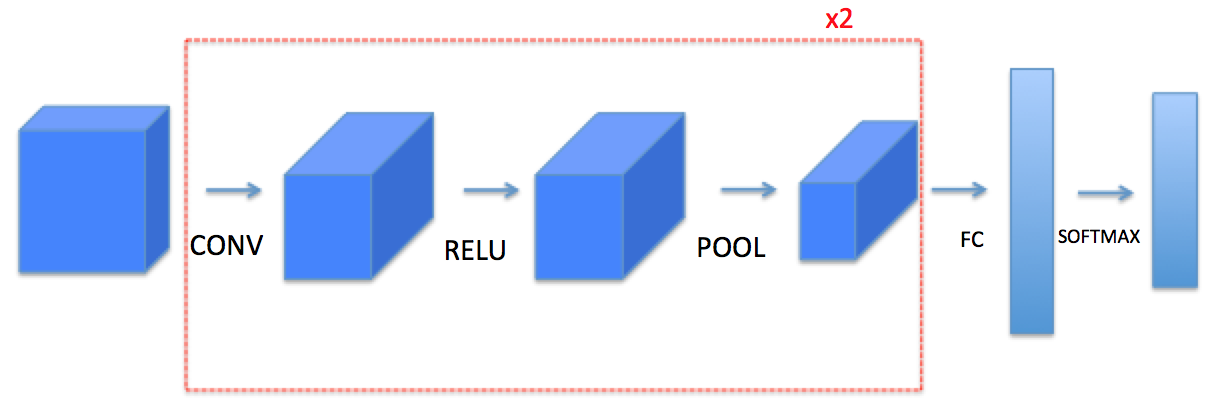
\includegraphics[width=14cm]{CNNExample.png}
    \caption{An example of CNN}
    \label{fig:CNNExample}
\end{figure}
~\\
Typically $n_H, n_W \downarrow; n_c \uparrow$\\
\\
Training set $(x^{(1)}, x^{(1)}), \cdots, (x^{(m)}, x^{(m)})$\\
Cost $J = \frac{1}{m}\sum_{i=1}^{m}L(\hat{y}^{(i)}, y^{(i)})$\\
Use gradient descent to optimize parameters to reduce $J$.\\

\emph{\textcolor{Bittersweet}{CNN being good at translation invariance (e.g., a picture of a cat shifted a couple of pixels to the right, is still pretty clearly a cat). The convolutional structure helps the neural network encode the fact that an image shifted a few pixels should result in pretty similar features and should probably be assigned the same label.}}


%_________________________________________________________________
\section{Deep convolutional models}

%
\subsection{Classic networks}
% Insert figures of each network architecture
\begin{itemize}
\item
    LeNet\\
    \textit{LeCun et al., 1998. Gradient-based learning applied to document recognition}\\
    $\sim$ 60K
    \begin{figure}[h]
        \centering
        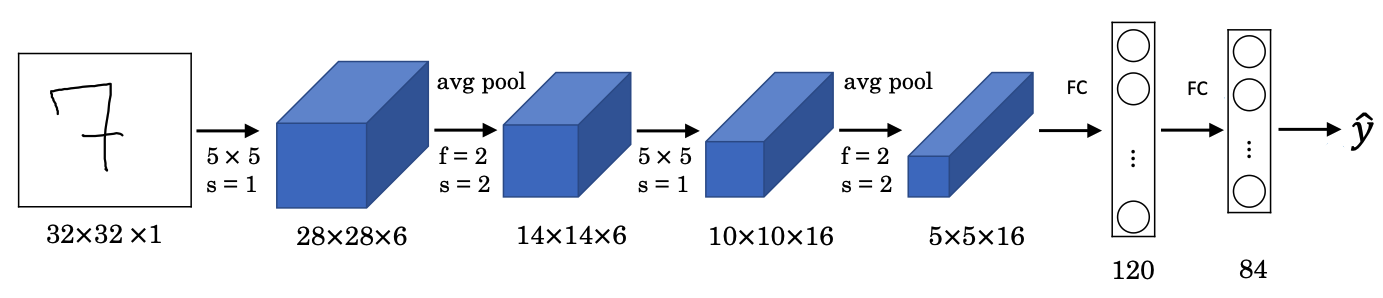
\includegraphics[width=14cm]{LeNet5.png}
        \caption{LeNet5}
        \label{fig:LeNet5}
    \end{figure}
\item
    AlexNet\\
    \textit{Krizhevsky et al., 2012. ImageNet classification with deep convolutional neural networks}\\
    $\sim$ 60M
    \begin{figure}[h]
        \centering
        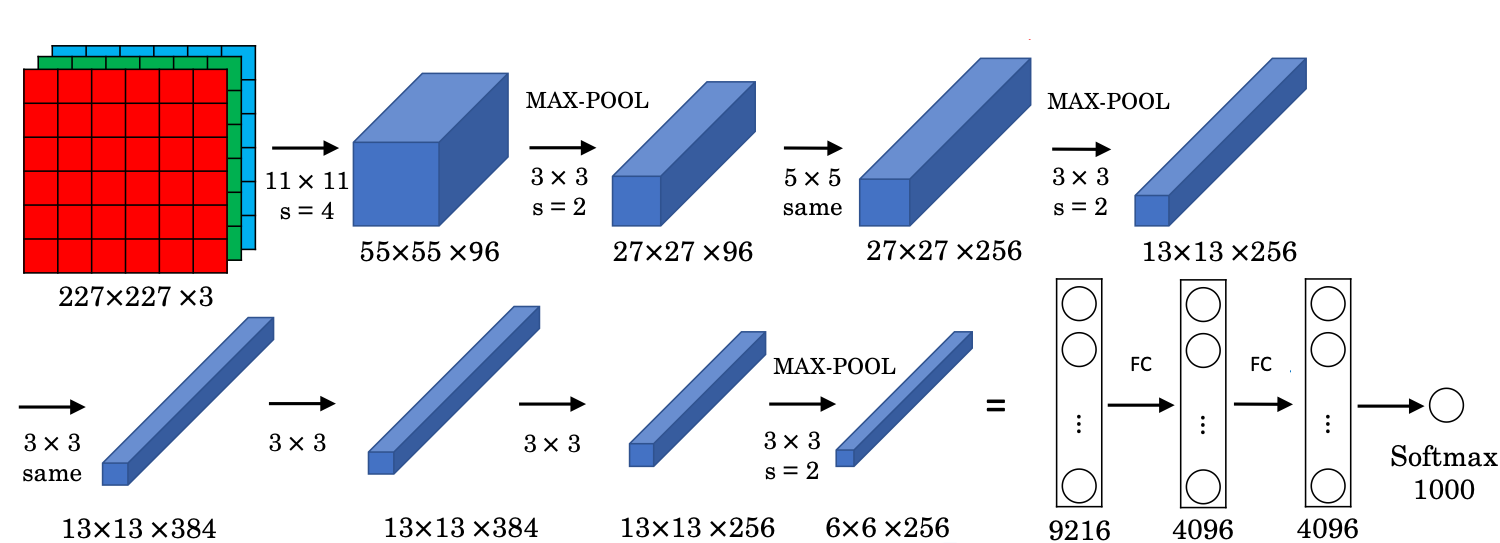
\includegraphics[width=14cm]{AlexNet.png}
        \caption{AlexNet}
        \label{fig:AlexNet}
    \end{figure}
\item
    VGG-16\\
    CONV = $3 \times 3$ filter, s = 1, same MAX-POOL = $2 \times2$ , s = 2\\
    $\sim$138M\\
    \textit{Simonyan \& Zisserman 2015. Very deep convolutional networks for large-scale image recognition}
    \begin{figure}[h]
        \centering
        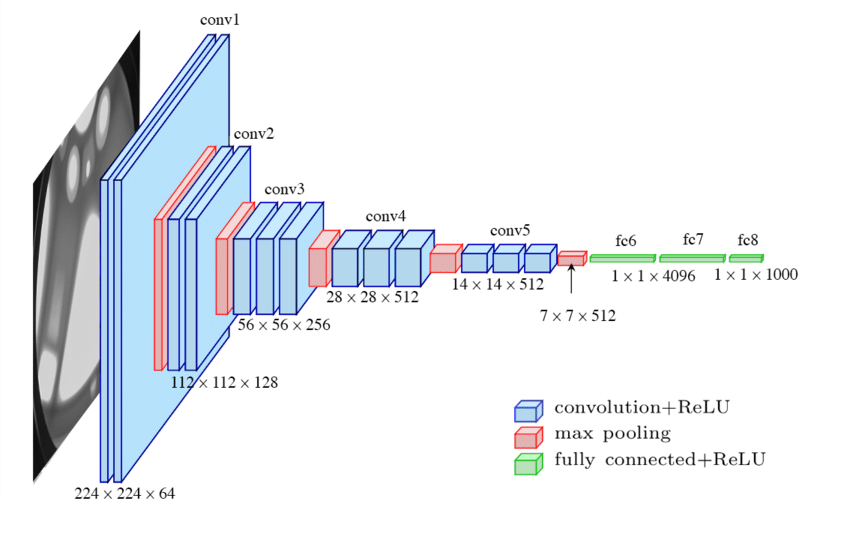
\includegraphics[width=14cm]{VGG16.png}
        \caption{VGG16}
        \label{fig:VGG16}
    \end{figure}
\item
    ResNets\\
    \textit{He et al., 2015. Deep residual networks for image recognition}\\
    The motivation of Residual Networks is actually to help us train very deep networks. Indeed, very deep neural networks are hard to train and a deeper network does not always imply lower training error.
    \begin{itemize}
    \item
        Residual block:\\
        ``short cut''/skip connection vs. ``main path''\\
        Two types of blocks:\\
        \begin{itemize}
        \item
        identity block
        \item
        convolutional block
        \end{itemize}
        \begin{figure}[h]
            \centering
            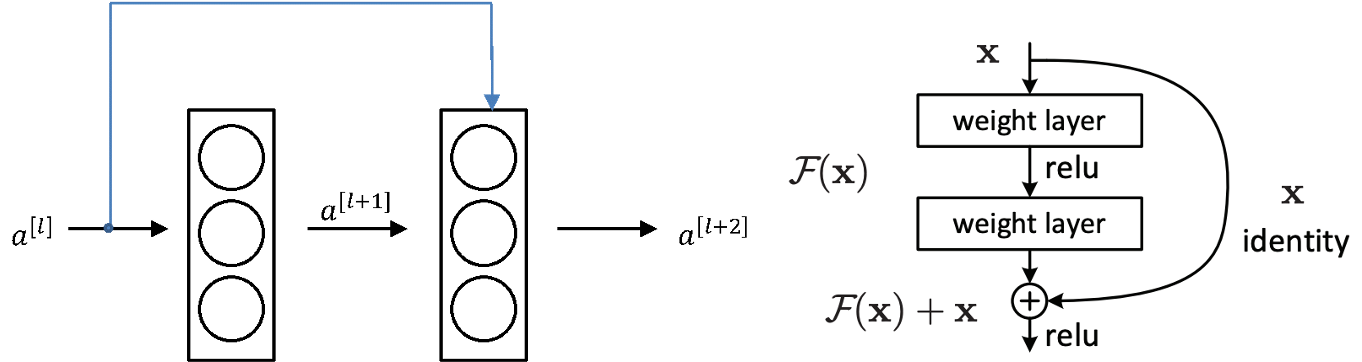
\includegraphics[width=14cm]{residualblock.png}
            \caption{Residual block}
            \label{fig:residualblock}
        \end{figure}
        \item
        ``Plain network'' $\rightarrow$ ``Residual networks''\\
        which helps with the vanishing and exploding gradient problems and allows to train much deeper neural networks without really appreciable loss in performance.
        \item
        Why do residual networks work?\\
        It's easy for those extra layers to learn the identity function, which kind of guaranteed not hurting the performance.\\\\
        In $a^{[l+2]} = g(z^{[l+2]} + a^{[l]})$, $z^{[l+2]}$ and $a^{[l]}$ suppose to have the same dimension, so very often the ``same'' convolutions are used. In case they have different dimensions, an extra weight matrix ($W_s$) is multiplied to $a^{[l]}$, or similarly a CONV layer in the shortcut path is used to resize the input to a different dimension, so that the dimensions match up in the final addition needed to add the shortcut value back to the main path. The CONV layer on the shortcut path does not use any non-linear activation function. Its main role is to just apply a (learned) linear function that reduces the dimension of the input, so that the dimensions match up for the later addition step.
    \end{itemize}
\item
    Inception Network (GoogLeNet)\\
    \textit{Lin et al., 2013. Network in network}\\
    Szegedy et al. 2014. Going deeper with convolutions
    \begin{figure}[h]
        \centering
        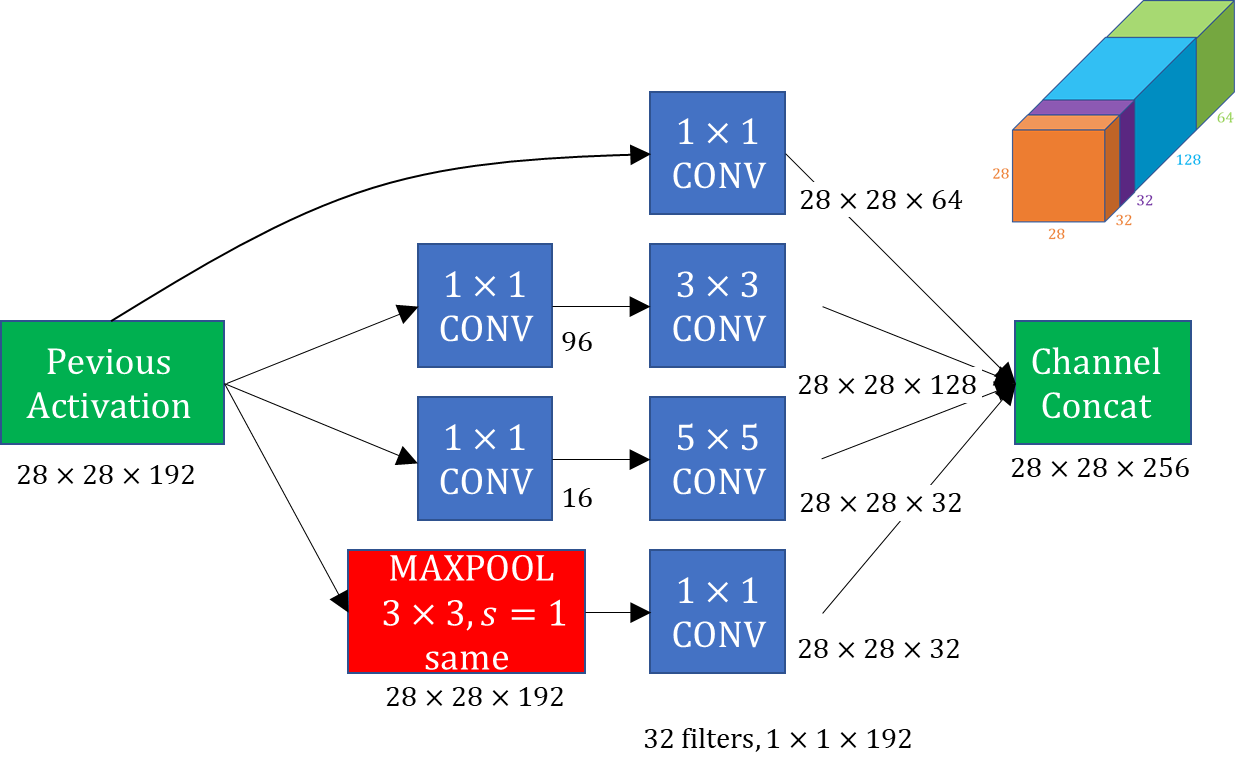
\includegraphics[width=12cm]{inception_module.png}
        \caption{ Inception module}
        \label{fig:inception_module}
    \end{figure}
    \begin{itemize}
        \item
        Network in network ($1 \times 1$ convolution)\\
        fully connected network applied to each of the positions across the channels $\rightarrow$ output \# filters $n_c^{[l+1]}$\\
        to shrink the hight ($n_H$) and width ($n_W$) $\rightarrow$ pooling\\
        to shrink the number of channels ($n_c$) $\rightarrow$ 32 $1 \times 1 \times 192$ filters\\
        The $1 \times 1$ convolution can also keep $n_c$ the same or increase it.
        \item
        Inception module\\
        Previous activation $\rightarrow$ \{CONV 1 $\times$ 1, CONV 1 $\times$ 1 + CONV 3 $\times$ 3,  CONV 1 $\times$ 1 + CONV 5 $\times$ 5, MAXPOOL same, etc.\} $\rightarrow$ Channel concat\\
        Instead of picking the filter sizes or pooling, do all of them and just concatenate the outputs (combination of the filters).
        \item
        The problem of computational cost\\
        $28 \times 28 \times 192 \xrightarrow[]{\text{CONV} 5 \times 5 ~ \text{same} ~ 32} 28 \times 28 \times 32$\\
        Cost: 32 filters of $5 \times 5 \times 192 \rightarrow  (28 \times 28 \times 32) \times (5 \times 5 \times 192)$ = 120M\\
        $28 \times 28 \times 192 \xrightarrow[]{\text{CONV} 1 \times 1 ~ \text{same} ~ 16} 28 \times 28 \times 16 \xrightarrow[]{\text{CONV} 5 \times 5 ~ \text{same} ~ 32} 28 \times 28 \times 32$, ``bottleneck layer''\\
        Cost: $ (28 \times 28 \times 16) \times 192 + (28 \times 28 \times 32) \times (5 \times 5 \times 116)$ = 10M
    \end{itemize}
     \begin{figure}[h]
        \centering
        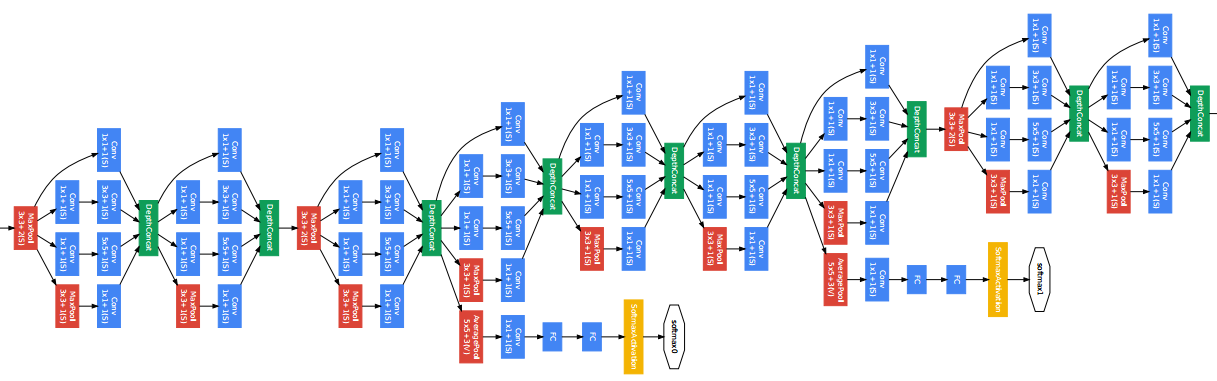
\includegraphics[width=14cm]{InceptionNet.png}
        \caption{ Inception network}
        \label{fig:Inception}
    \end{figure}
\end{itemize}

%
\subsection{MobileNet}

\begin{itemize}
\item
    Low computational cost at deployment
\item
    Useful for mobile and embedded vision applications
\item
    Key idea: Normal vs. depthwise-separable convolutions
    \begin{figure}[h]
    \centering
    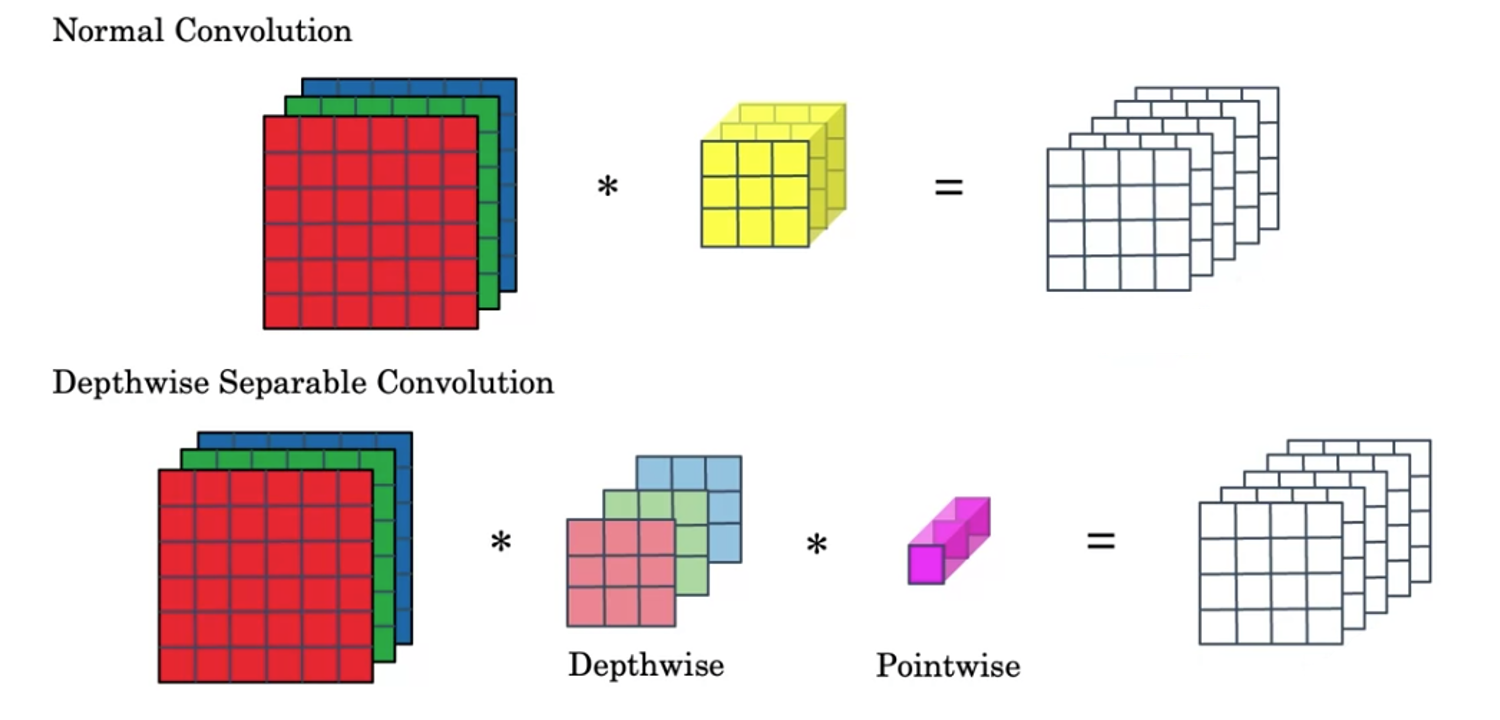
\includegraphics[width=12cm]{depthwiseSeeparableC.png}
    \caption{Normal vs. depthwise-separable convolution}
    \label{fig:depthwiseSeeparableC}
    \end{figure}

    \begin{itemize}
    \item
    Normal convolution:\\
    $(n \times n \times n_c, 6\times 6 \times 3) * (f \times f \times n_c \times n'_c, 3 \times 3 \times 3 \times 5) = (n_{out} \times n_{out} \times n'_c, 4 \times 4 \times 5)$\\
    Computational cost = \#filter parameters $\times$  \#filter positions $\times$ \# filters\\
    $3 \times 3 \times 3 \times 4 \times 4 \times 5 = 2160$
    \item
    depthwise-separable convolutions:\\
    Depthwise Convolution:\\
    $(n \times n \times n_c, 6\times 6 \times 3) * (f \times f, 3 \times 3) = (n_{out} \times n_{out} \times n_c, 4 \times 4 \times 3)$\\
    Computational cost = \#filter parameters $\times$  \#filter positions $\times$ \# filters\\
    $3 \times 3 \times 4 \times 4 \times 3 = 432$\\
    Pointwise Convolution:\\
    $(n_{out} \times n_{out} \times n_c, 4\times 4 \times 3) * (f \times f \times n_c \times n'_c, 1 \times 1 \times 3 \times 5) = (n_{out} \times n_{out} \times n_c', 4 \times 4 \times 5)$\\
    Computational cost = \#filter parameters $\times$  \#filter positions $\times$ \# filters\\
    $1 \times 1 \times 3 \times 4 \times 4 \times 5 = 240$\\
    \item
    The ratio of the cost for the depthwise separable convolution compared to the normal convolution:\\
    $\frac{1}{n'_c} + \frac{1}{f^2}$
    \end{itemize}
\end{itemize}

%%
\subsubsection{MobileNet architecture}
MobileNet V1:\\
Input $\rightarrow$ 13 times depthwise convolutional operation  $\rightarrow$ Pooling  $\rightarrow$ FC  $\rightarrow$ Softmax\\
\\
MobileNet V2:\\
Input $\rightarrow$ 17 times Residual connections $\rightarrow$ Pooling  $\rightarrow$ FC  $\rightarrow$ Softmax\\
Residual connection (Bottleneck): Expansion $\rightarrow$ Depthwise $\rightarrow$ Projection (pointwise).\\
More computation inside the residual connection, then project back down to a smaller size outside the block, which allows the neural network to learn richer and more complex functions, while also keeping the amounts of memory that is the size of the activations passed from layer to layer, relatively small.
\begin{figure}[h]
    \centering
    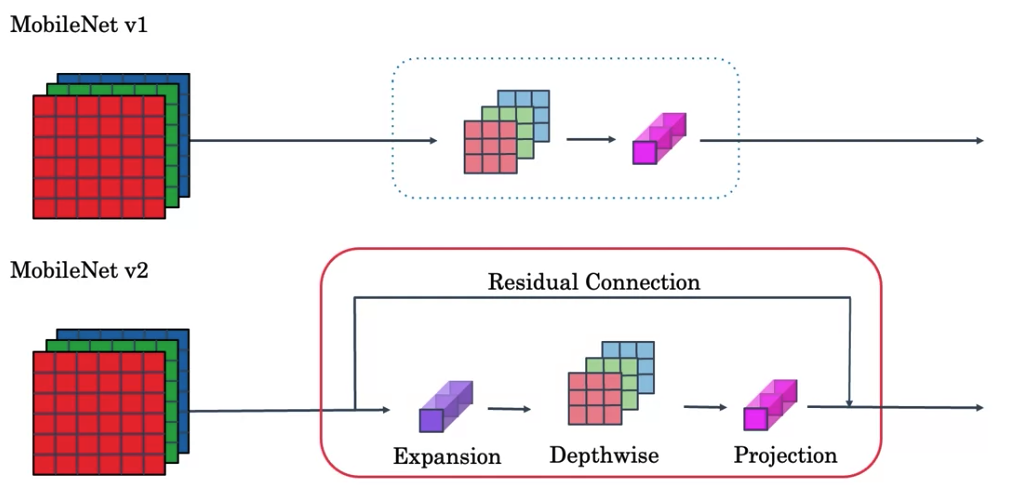
\includegraphics[width=12cm]{mobilenetv1.png}
    \caption{MobileNetV1 vs. MobileNetV2}
    \label{fig:mobilenetv1}
\end{figure}
\begin{figure}[h]
    \centering
    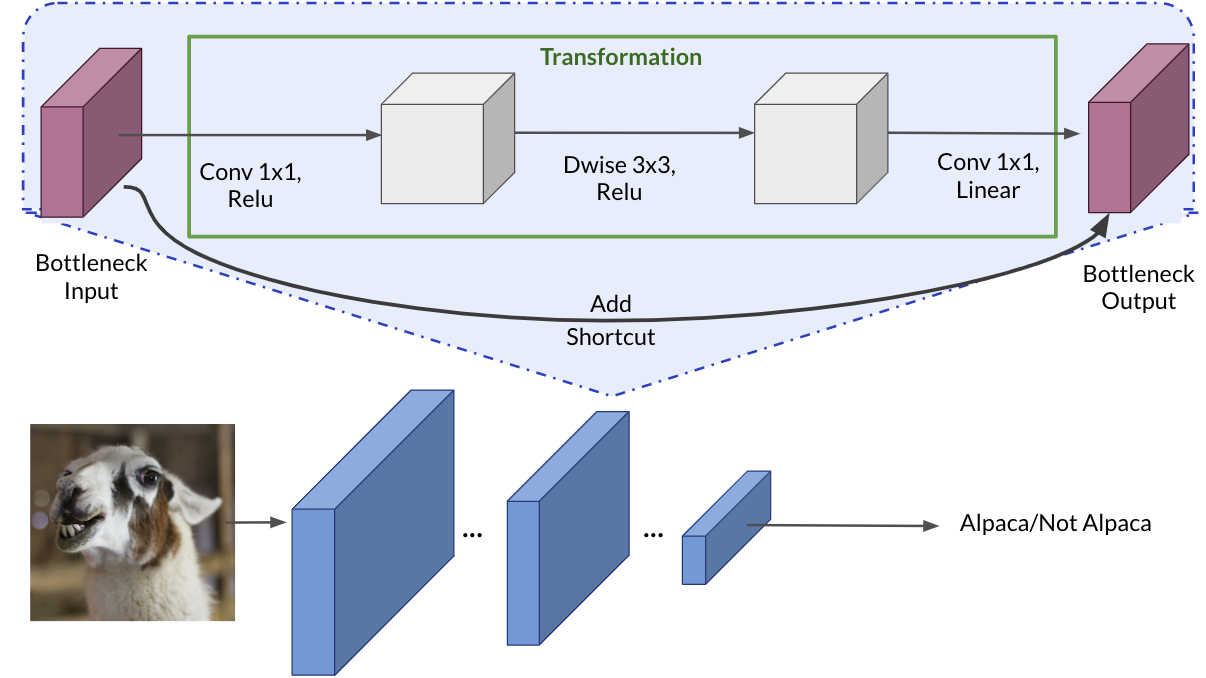
\includegraphics[width=12cm]{mobilenetv2.png}
    \caption{MobileNetV2 architecture}
    \label{fig:mobilenetv2}
\end{figure}

\subsubsection{EfficientNet}
r: resolution\\
d: depth\\
w: width\\
Given a particular computational budget, what's the good choice of r, d and w?\\
Baseline vs. Compound scaling, to scale up or down the neural networks based on the resources of a device.\\

%
\subsection{Transfer learning}
Rather than training the weights from scratch (random initialization), download weights that someone else has already trained on the network architecture and use that as pre-training and transfer that to a new task that you might be interested in.\\
To adapt the classifier to new data: Delete the top layer, add a new classification layer, and train only on that layer. When freezing layers, avoid keeping track of statistics (like in the batch normalization layer). Fine-tune the final layers of your model to capture high-level details near the end of the network and potentially improve accuracy.
\begin{itemize}
\item
Small dataset:\\
Replace the softmax layer with your own application. Freeze the weights of all the previous layers, and re-train the weights at the softmax layer, e.g. trainable parameter, freeze, etc. in DL frameworks.\\
Pre-compute the activation of the layer before the softmax layer and save them to disk. Using this fixed function and then training a shallow softmax model from this feature vector to make a prediction.
\item
Large dataset:\\
Freeze fewer (bigger data) earlier layers, and re-train weights of the later layers.
\item
A lot of data:\\
Retrain the whole model.
\end{itemize}

%
\subsection{Data Augmentation}
\begin{itemize}
\item[]
Mirroring
\item[]
Random Cropping
\item[]
Rotation, Shearing, Local warping, etc.
\item[]
Color shifting\\
PCA color augmentation
\item[]
Implementing distortions during training
\end{itemize}

%
\subsection{State of computer vision}
Data vs. hand-engineering\\
Little data $\xrightarrow{\hspace*{8cm}}$ Lots of data\\
Objection detection \ \ \  Image recognition \ \ \ Speech recognition\\
More hand-engineering(``hacks'') $\xrightarrow{\hspace*{2cm}}$ Less hand-engineering (Simpler algorithms)\\
\\
Two sources of knowledge
\begin{itemize}
\item
Labeled data
\item
Hand engineered features / network architectures / other components
\end{itemize}

Tips for doing well on benchmarks/winning competitions
\begin{itemize}
\item
Ensembling\\
Train several networks (3 -- 15) independently and average their outputs ($\hat{y}$).
\item
Multi-crop at test time\\
Run classifier on multiple versions of test images and average results, e.g., 10--crop (1 central, 4 corners, 1 mirror central, 4 mirror corners).
\item
Use architectures of networks published in the literature
\item
Use open source implementations if possible
\item
Use pre-trained models and fine-tune on your dataset
\end{itemize}


%_________________________________________________________________
\section{Object Detection}
What objects are in this image and where in the image are those objects located?
%
\subsection{Object localization}
What are localization and detection?\\
Image classification (1 object).\\
Classification with localization: figuring out where in the image is the object (1 object).\\
Detection: detect all the objects and localize them all (multiple objects maybe in different categories).

\subsubsection{Classification with localization}
Input $\rightarrow$ ConvNets $\rightarrow$ softmax (class labels) + bounding box\\
bounding box: $b_x, b_y, b_w, b_h$\\
\\
Defining the target label y:\\
$y = \begin{bmatrix} P_c \\ b_x\\ b_y\\ b_w\\ b_h \\ C_1 \\ C_2 \\ C_3
\end{bmatrix}$, e.g., $y = \begin{bmatrix} 1 \\ b_x\\ b_y\\ b_w\\ b_h \\ 0 \\ 1 \\0
\end{bmatrix}$, $y = \begin{bmatrix} 0 \\ ? \\ ?\\ ?\\ ? \\ ? \\ ? \\?
\end{bmatrix}$\\
\\
The loss function (example with the SQE)
\begin{equation}
L(\hat{y}, y) = \left\{ 
    \begin{array}{rll}
   \sum_{t=1}^8(\hat{y_t} - y_t)^2 & \text{if} & y_1 =1 \\
    (\hat{y_1} - y_1)^2 & \text{if} &y_1 = 0 \\
    \end{array} \right.
\end{equation}

\begin{figure}[h]
    \centering
    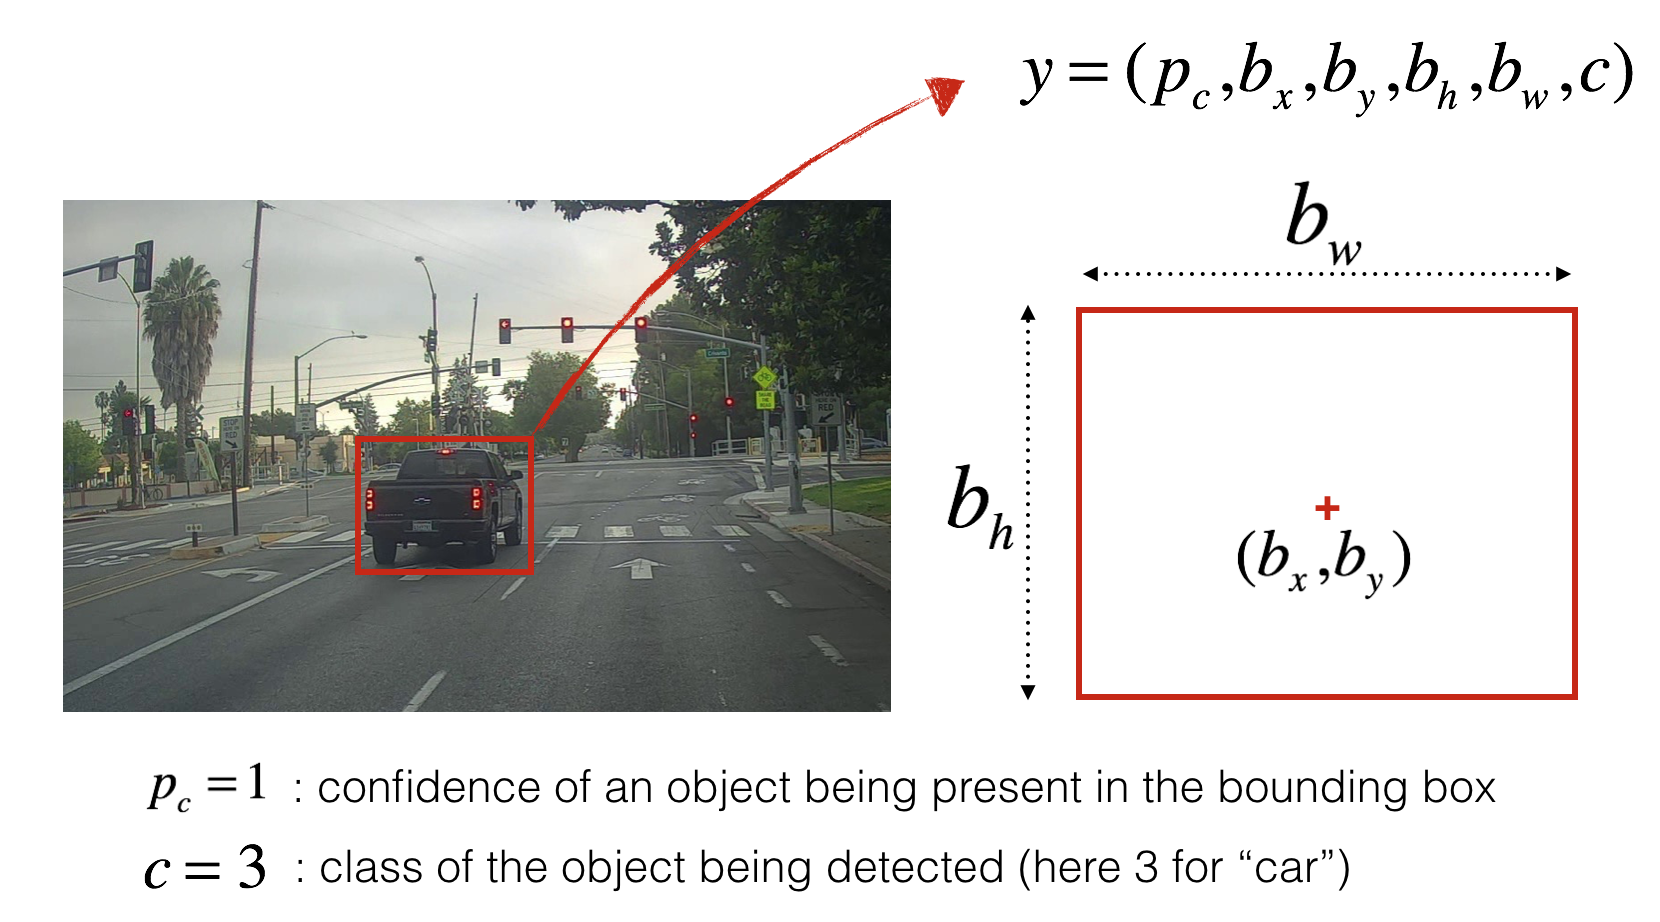
\includegraphics[width=10cm]{box_label.png}
    \caption{Definition of a box}
    \label{fig:boxlabel}
\end{figure}

\subsubsection{Landmark detection}
A neural network output $X$ and $Y$ coordinates of important points in an image, sometimes called landmarks, that you want the neural networks to recognize.\\
\underline{Example}: face contour for AR. Input $\rightarrow$ ConvNets $\rightarrow$ 129 output units: face? + $l_{1x}, l_{1y}, l_{2x}, l_{2y}, \cdots, l_{64x}, l_{64y}$.
\underline{Example}: Pose/emotion detection. 

%
\subsection{Object detection algorithms}

%%
\subsubsection{Sliding windows detection}

Train a ConvNet on closely cropped examples of cars $\rightarrow$ Sliding windows detection (take a small rectangular region and input it to the ConvNet) $\rightarrow$ Go through the entire image $\rightarrow$ repeat with a larger window.
%%
\subsubsection{Convolutional implementation of sliding windows}
Turning FC layer into convolutional layers.\\
Instead of doing it sequentially, implement convolutionally all at a time.\\
\begin{itemize}
\item
$(14 \times 14 \times 3) \xrightarrow[5 \times 5]{} (10 \times 10 \times 16) \xrightarrow[2 \times 2]{\text{MAX~POOL}} (5 \times 5 \times 16) \xrightarrow[]{\text{FC}} 400 \xrightarrow[]{\text{FC}} 400 \rightarrow y ~ \text{softmax}(4)$
\item
$(14 \times 14 \times 3) \xrightarrow[5 \times 5]{} (10 \times 10 \times 16) \xrightarrow[2 \times 2]{\text{MAX~POOL}} (5 \times 5 \times 16) \xrightarrow[5 \times 5 \times 16 \times 400]{\text{FC}} 1 \times 1 \times 400 \xrightarrow[1 \times 1 \times 400 \times 400]{\text{FC}} 1 \times 1 \times 400 \xrightarrow[1 \times 1 \times 400 \times 4]{\text{FC}}  y ~ \text{softmax}(1\times 1 \times 4)$
\item
$(16 \times 16 \times 3) \xrightarrow[5 \times 5]{} (12 \times 12 \times 16) \xrightarrow[2 \times 2]{\text{MAX~POOL}} (6 \times 6 \times 16) \xrightarrow[5 \times 5]{\text{FC}} 2 \times 2 \times 400 \xrightarrow[1 \times 1]{\text{FC}} 2 \times 2 \times 400 \xrightarrow[1 \times 1]{\text{FC}}  y ~ \text{softmax}(2\times 2 \times 4)$
\item
$(28 \times 28 \times 3) \xrightarrow[5 \times 5]{} (24 \times 24 \times 16) \xrightarrow[2 \times 2]{\text{MAX~POOL}} (12 \times 12 \times 16) \xrightarrow[5 \times 5]{\text{FC}} 8 \times 8 \times 400 \xrightarrow[1 \times 1]{\text{FC}} 8 \times 8 \times 400 \xrightarrow[1 \times 1]{\text{FC}}  y ~ \text{softmax}(8\times 8 \times 4)$
\end{itemize}
~\\
\textit{Sermanet et al., 2014, OverFeat: Integrated recognition, localization and detection using convolutional networks}
%%
\subsubsection{Bounding box predictions: YOLO}
Place down a grid on the input image, apply the image classification and localization algorithm to each of the grids.\\
\begin{figure}[h]
    \centering
    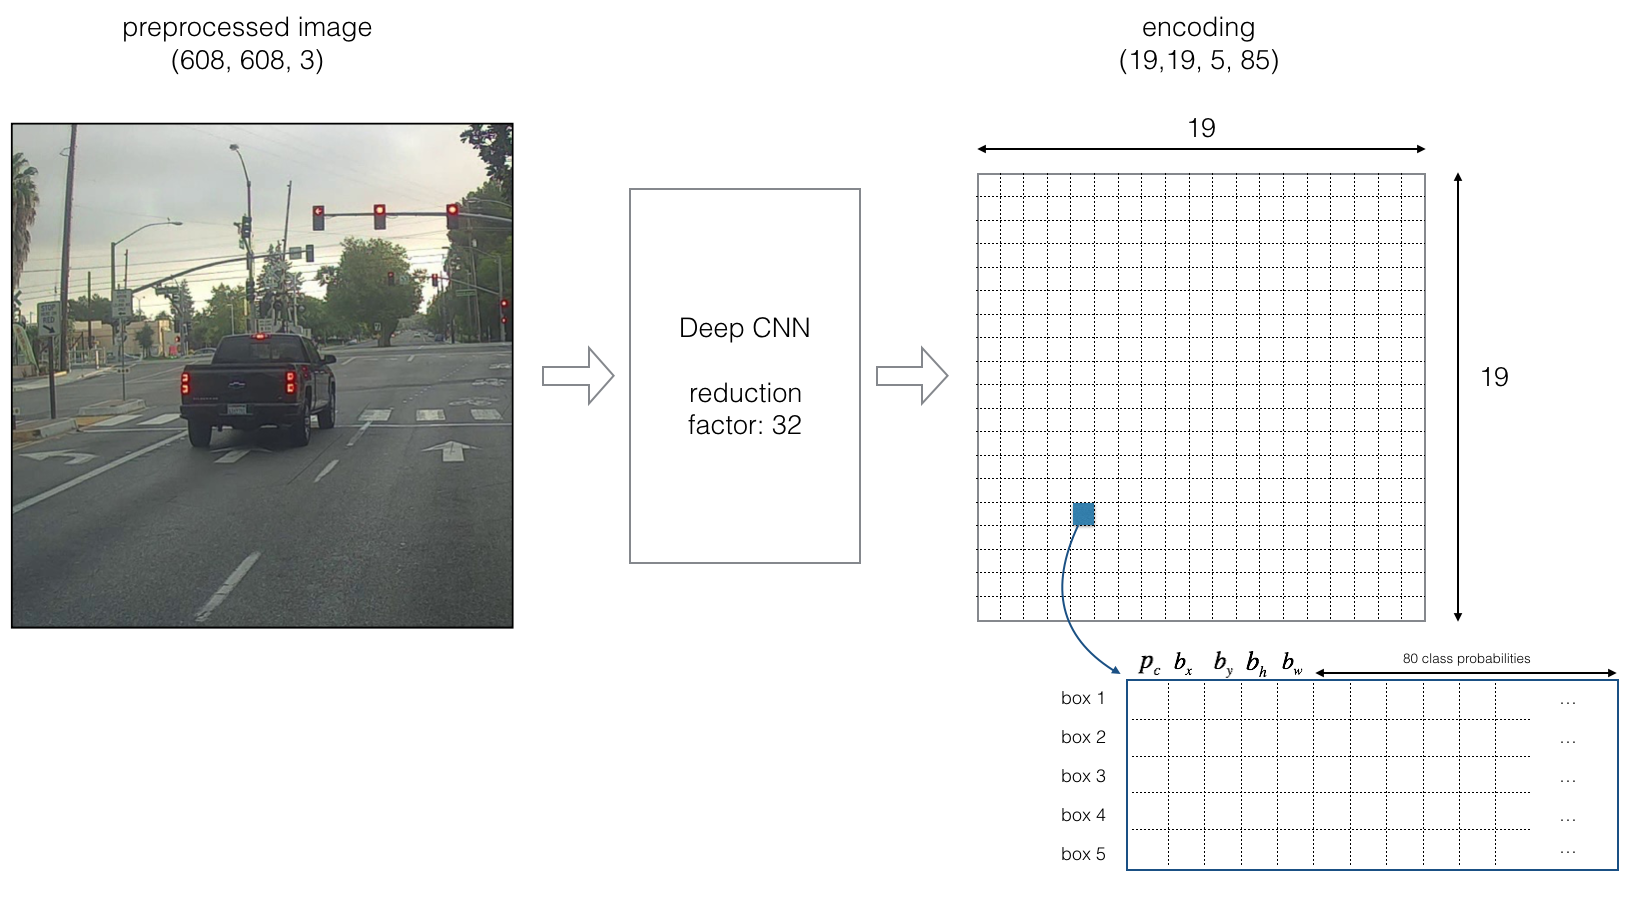
\includegraphics[width=14cm]{YOLO.png}
    \caption{Encoding architecture for YOLO}
    \label{fig:YOLO}
\end{figure}

\textit{Redmon et al., 2015, You Only Look Once: Unified real-time object detection}\\
\underline{Example}:
\begin{itemize}
\item
    Input image $(608, 608, 3)$
\item
    The input image goes through a CNN, resulting in a $(19, 19, 5, 85)$ dimensional output.
\item
    After flattening the last two dimensions, the output is a volume of shape (19, 19, 425):
    \begin{itemize}
    \item
    Each cell in a $19 \times19$ grid over the input image gives 425 numbers.
    \item
    $425 = 5 \times 85$ because each cell contains predictions for 5 boxes, corresponding to 5 anchor boxes.
    \item
    $85 = 5 + 80$ where 5 is because $(p_c, b_x, b_y, b_w, b_h)$ has 5 numbers, and 80 is the number of classes we'd like to detect
    \end{itemize}
\item
    select only few boxes based on:
    \begin{itemize}
    \item
    Score-thresholding: throw away boxes that have detected a class with a score less than the threshold
    \item
    Non-max suppression: Compute the Intersection over Union and avoid selecting overlapping boxes
    \end{itemize}
\end{itemize}
~\\
\textbf{Intersection over union (IoU)}\\
IoU is a measure of the overlap between two bounding boxes.\\
IoU = $\displaystyle\frac{\text{size of intersection}}{\text{size of union}}$\\

``Correct'' if IoU $\ge$ 0.5
\begin{figure}[h]
    \centering
    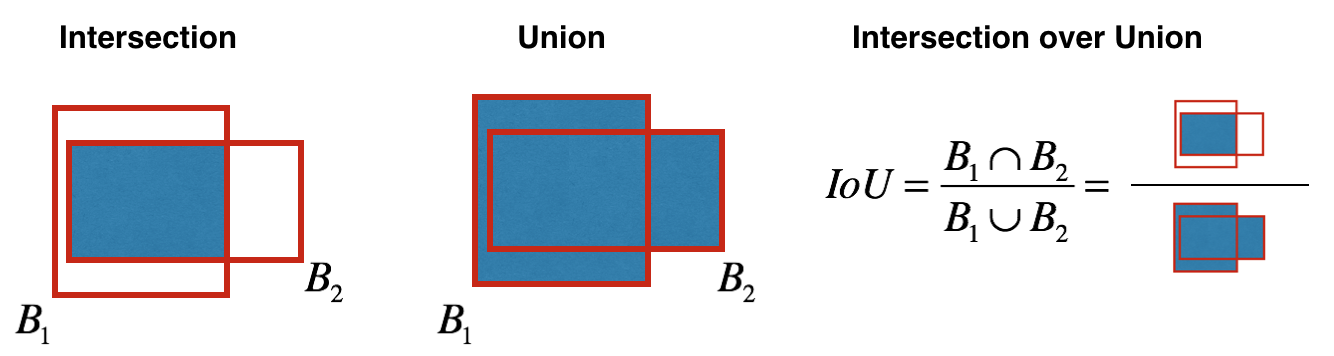
\includegraphics[width=12cm]{iou.png}
    \caption{Definition of``Intersection over Union''}
    \label{fig:iou}
\end{figure}

\textbf{Non-max suppression example}\\
Output the maximal probabilities but suppress the close-by ones that are non-maximal.\\
\\
For multiple detections of each object, it looks at the probabilities associated with each of these detections (e.g., $p_c$).\begin{enumerate}
\item
Each output prediction is e.g., $y = \begin{bmatrix} p_c \\ b_x\\ b_y\\ b_w\\ b_h \end{bmatrix}$\\
Discard all boxes with $p_c \le 0.6$
\item
While there are any remaining boxes:
\begin{itemize}
\item
Pick the box with the largest $p_c$\\
Output that as a prediction.
\item
Discard any remaining box with IoU $\ge$ 0.5
\end{itemize}
\end{enumerate}
~\\
\textbf{Anchor boxes}\\
Overlapping objects: Pre-define different anchor boxes.\\
With two anchor boxes:\\
Each object in training image is assigned to grid cell that contains object's midpoint and anchor box for the grid cell with highest IoU. (grid cell, anchor box)\\
e.g., $y = {\begin{bmatrix} p_c \\ b_x \\ b_y \\ b_w \\ b_h \\ c_1 \\ c_2 \\ c_3 \\ p_c \\ b_x \\ b_y \\ b_w \\ b_h \\ c_1 \\ c_2 \\ c_3 \end{bmatrix}}$\\
Anchor box selection: To use K-means algorithm to group together types of objects' shapes.

%%
\subsubsection{Region proposal: R-CNN}
\textit{Girshik et. al, 2013, Rich feature hierarchies for accurate object detection and semantic segmentation}\\
\textit{Girshik, 2015. Fast R-CNN}\\
\textit{Ren et. al, 2016. Faster R-CNN}\\
Run segmentation algorithms to figure out what could be objects.
\begin{itemize}
\item[]
R-CNN\\
Propose regions. Classify proposed regions one at a time. Output label + bounding box.
\item[]
Fast R-CNN\\
Propose regions. Use convolution implementation of sliding windows to classify all the proposed regions.
\item[]
Faster R-CNN\\
Use convolutional network to propose regions.
\end{itemize}

%
\subsection{Semantic segmentation with U-Net}
Instead of just giving a single class label (and coordinates needed to specifying bounding box), to label every single pixel individually.\\
Per-pixel class labels.\\
Deep learning for semantic segmentation: Blow up small activation to bigger activation.
\begin{itemize}
\item
Semantic image segmentation predicts a label for every single pixel in an image.
\item
U-Net uses an equal number of convolutional blocks and transposed convolutions for downsampling and upsampling.
\item
Skip connections are used to prevent border pixel information loss and overfitting in U-Net.
\end{itemize}
%%
\subsubsection{Transpose convolutions}
place the filter on the output.
\begin{figure}[h]
    \centering
    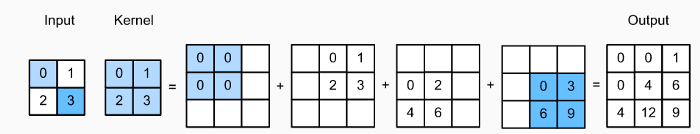
\includegraphics[width=14cm]{transpose_convolution.png}
    \caption{An example of transpose convolution computation}
    \label{fig:transposeCON}
\end{figure}

%%
\subsubsection{U-Net architecture intuition}
U-net uses a matching number of convolutions for downsampling the input image to a feature map, and transposed convolutions for upsampling those maps back up to the original input image size.\\
It also adds \emph{skip connections}, to retain information that would otherwise become lost during encoding. Skip connections send information to every upsampling layer in the decoder from the corresponding downsampling layer in the encoder, capturing finer information while also keeping computation low.
\\
\textit{Ronneberger et al., 2015, U-Net: Convolutional Networks for Biomedical Image Segmentation}
%figure
\begin{figure}[h]
    \centering
    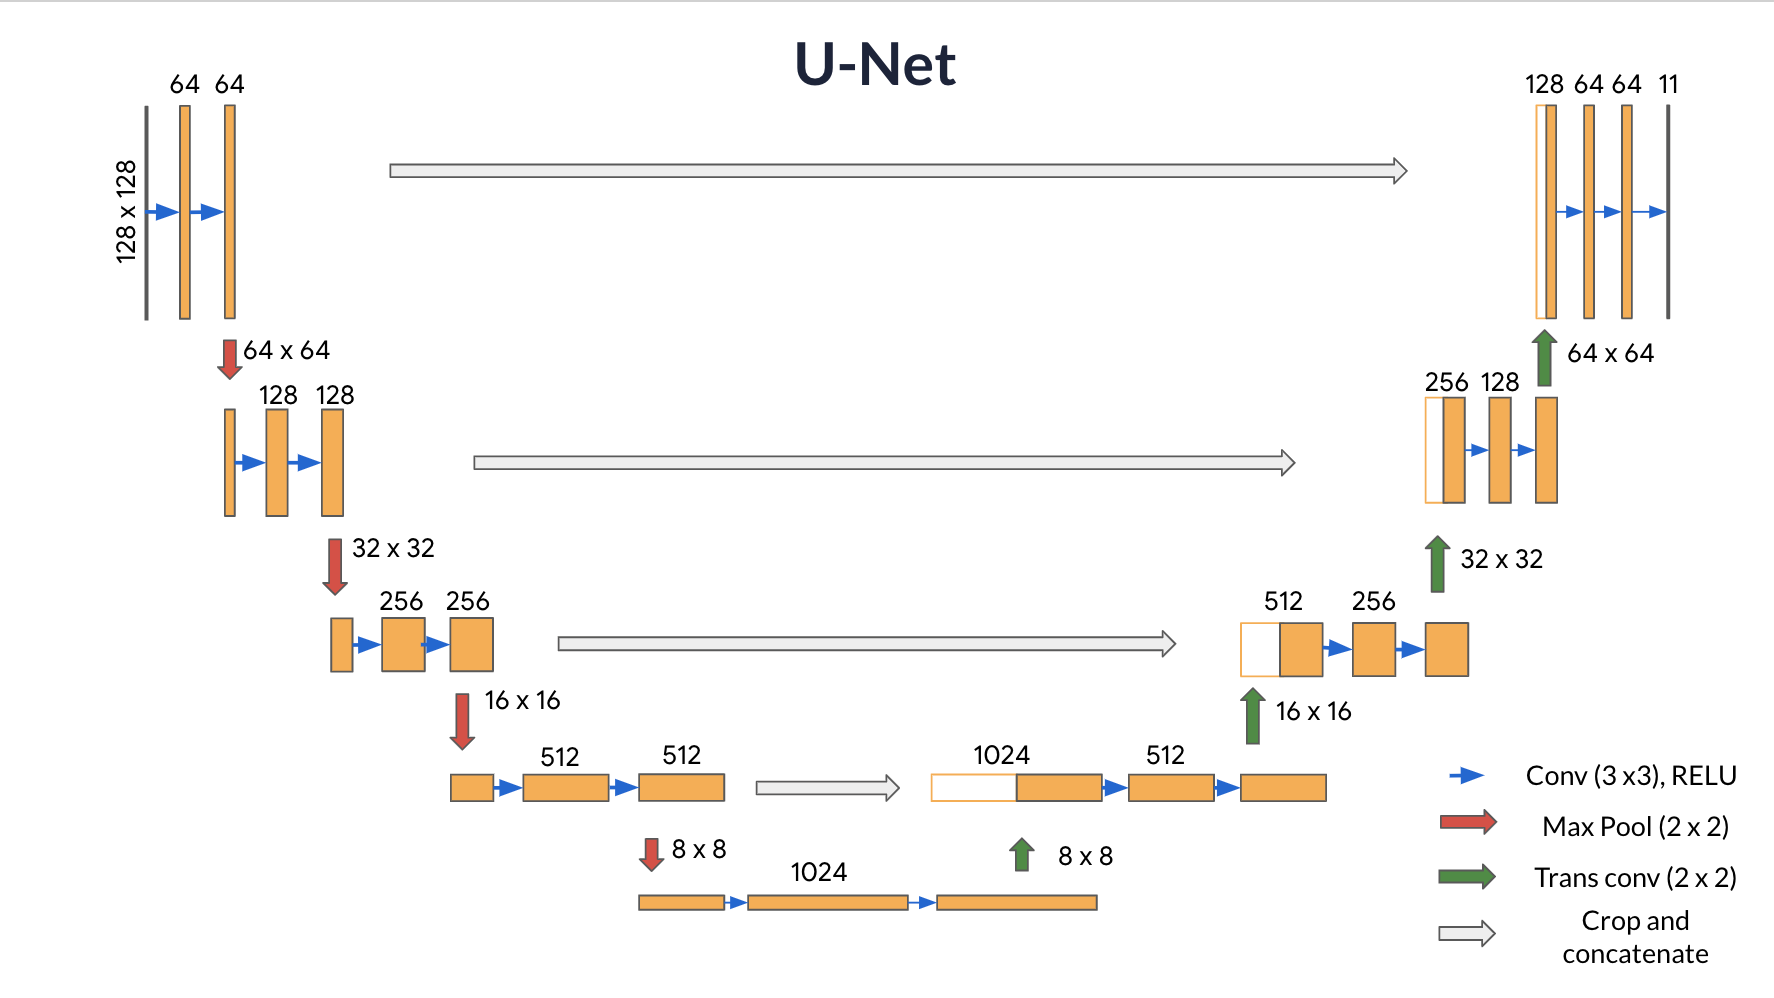
\includegraphics[width=16cm]{unet.png}
    \caption{U-Net Architecture}
    \label{fig:unet}
\end{figure}


%_________________________________________________________________
\section{Face recognition \& Neural style transfer}
%
\subsection{Face recognition}
Face verification vs. face recognition
\begin{itemize}
\item
Verification
    \begin{itemize}
    \item
    Input image, name/ID
    \item
    Output whether the input image is that of the claimed person
    \end{itemize}
\item
Recoginition
    \begin{itemize}
    \item
    Has a database of K persons
    \item
    Get an input image
    \item
    Output ID if the image is any of the K persons (or ``not recognized'')
    \end{itemize}
\end{itemize}

%
\subsection{One shot learning}
Learning from one example to recognize the person again.\\
Learning a ``similarity'' function\\
d(img1, img2) = degree of difference between images\\
Verification:\\
If d(img1, img2) $\le \tau$: ``same'';\\
If d(img1, img2) $\ge \tau$: ``different''.\\

%
\subsection{Siamese network}

\textit{Taigman et. al., 2014. DeepFace closing the gap to human level performance}\\
Two input images: $x^{(1)}, x^{(2)}$\\
``encoding'' of the images: $f(x^{(1)}), f(x^{(2)})$\\
$d(x^{(1)}, x^{(2)}) = \lVert f(x^{(1)}) - f(x^{(2)}) \rVert_2^2$\\
\\
Parameters of NN define an encoding $f(x^{(1)})$\\
Learn parameters so that:\\
If $x^{(1)}, x^{(2)}$ are the same person, $\lVert f(x^{(1)}) - f(x^{(2)}) \rVert_2^2$ is small\\
If $x^{(1)}, x^{(2)}$ are different  persons, $\lVert f(x^{(1)}) - f(x^{(2)}) \rVert_2^2$ is large\\

\begin{figure}[h]
    \centering
    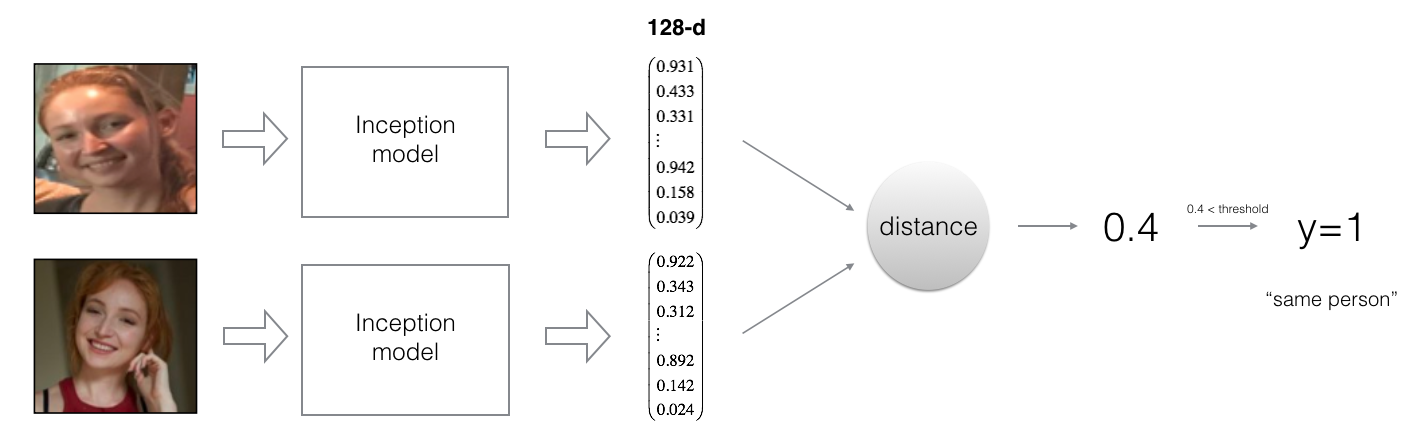
\includegraphics[width=16cm]{siamese.png}
    \caption{Computing the distance between two encodings and thrsholding}
    \label{fig:siamese}
\end{figure}

%%
\subsubsection{Triplet loss}
\textit{Schroff et al.,2015, FaceNet: A unified embedding for face recognition and clustering}\\
Learning objective:\\
``push'' the encodings of two images of the same person (Anchor and Positive) closer together, while ``pulling'' the encodings of two images of different persons (Anchor, Negative) further apart.\\
\\
A is an ``Anchor'' image -- a picture of a person.\\
P is a ``Positive'' image -- a picture of the same person as the Anchor image.\\
N is a ``Negative'' image -- a picture of a different person than the Anchor image.\\
\\
$\lVert f(A) - f(P) \rVert^2 \le \lVert f(A) - f(N) \rVert^2$\\
$\lVert f(A) - f(P) \rVert^2 - \lVert f(A) - f(N) \rVert^2 + \alpha \le  0$\\
$\alpha$ is the margin hyperparameter, which pushes the anchor-positive pair and the anchor-negative pair further away from each other. An image $A^{(i)}$  of an individual is closer to the Positive  $P^{(i)}$ than to the Negative image  $N^{(i)}$ by at least a margin $\alpha$\\
\\
Given triplets images, $(A, P, N)$:\\
Loss function:
\begin{align}
L(A,P,N) = \max(\lVert f(A) - f(P) \rVert^2 - \lVert f(A) - f(N) \rVert^2 + \alpha,  0)
\end{align}
Cost function:\\
$J = \sum_{i=1}^{m}L(A^{(i)},P^{(i)},N^{(i)})$\\
\\
Multiple pictures of the same person are needed, e.g., training set: 10k pictures of 1k persons.\\
\\
Choosing the triplets (A, P, N)\\
During training, if (A, P, N) are chosen randomly, $d(A,P) + \alpha \le d(A,N)$ is easily satisfied.\\
Choose triplets that are ``hard'' to train on.\\
It's only by choosing ``hard'' to triplets that the gradient descent procedure has to do some work to try to push these quantities further away from those quantities.

%
\subsection{Face verification and binary classification}
\textit{Taigman et. al., 2014. DeepFace closing the gap to human level performance}\\
Input: two images.\\
Learning the similarity function: Take a pair of Siamese neural networks and have them both compute the embeddings, then have these be input to a logistic regression unit for a prediction.
\begin{align}
\hat{y} &= \sigma(\sum_{k=1}^K w_k \lvert f(x^{(i)})_k - f(x^{(j)})_k \rvert+ b)\\
\hat{y} &= \sigma(\sum_{k=1}^K w_k \frac{(f(x^{(i)})_k - f(x^{(j)})_k)^2}{f(x^{(i)})_k + f(x^{(j)})_k}+ b)
\end{align}

\emph{\textcolor{Bittersweet}{Pre-compute the encoding and then use that to make a prediction.}}

%
\subsection{Neural style transfer}
The optimization algorithm updates the pixel values rather than the neural network's parameters.

\begin{itemize}
\item
An algorithm that given a content image and a style image can generate an artistic image.
\item
It uses representations (hidden layer activations) based on a pre-trained ConvNet.
\item
The content cost function is computed using one hidden layer's activations.\\
The style cost function for one layer is computed using the Gram matrix of that layer's activations. The overall style cost function is obtained using several hidden layers.
\item
Optimizing the total cost function results in synthesizing new images.
\end{itemize}

Images: Content; Style; Generated image.

%%
\subsubsection{What are deep ConvNets learning?}
Visualizing deep layers\\
\textit{Zeiler and Fergus., 2013, Visualizing and understanding convolutional networks}\\
\\
The shallower layers of a ConvNet tend to detect lower-level features such as edges and simple textures.\\
The deeper layers tend to detect higher-level features such as more complex textures and object classes.
%%
\subsubsection{Neural style transfer cost function}
\textit{Gatys et al., 2015. A neural algorithm of artistic style}\\
\begin{align}
J(G) = \alpha J_{\text{Content}}(C, G) + \beta J_{\text{Style}}(C, G)
\end{align}
$\alpha$ and $\beta$ are hyperparameters that control the relative weighting between content and style.\\
~\\
Find the generated image G

\begin{enumerate}
\item
    Initiate G randomly\\
    G: $100 \times 100 \times 3$
\item
    Use gradient descent to minimize $J(G)$\\
    $G := G -  \frac{\partial J(G)}{\partial G}$
\item
    Content cost function
    \begin{itemize}
     \item
        To choose hidden layer $l$ to compute content cost (represent the content of an image).\\
        A layer in the middle of the network -- neither too shallow nor too deep. This ensures that the network detects both higher 	    level and lower level features.
    \item
        Use pre-trained ConvNet. (e.g., VGG network)
    \item
        Let $a^{[l](C)}$ and $a^{[l](G)}$ be the activation of layer $l$ on the images
    \item
        If $a^{[l](C)}$ and $a^{[l](G)}$ are similar, both images have similar content
        \begin{align}
        J_{\text{Content}}^{[l]}(C, G) = \frac{1}{2}\lVert a^{[l](C)} - a^{[l](G)}\rVert^2
        \end{align}    
    \end{itemize}
\item
    Style cost function
    \begin{itemize}
    \item
    Say you are using layer $l$'s activation to measure ``style''.
    \item
    Define style as correlation between activations across channels.\\
    How correlated are the activations across different channels?\\
    How often the high-level features occur or don't occur together in different parts of an image (unnormalized cross covariance).\\
    \\
    \textbf{Style matrix} (Gram matrix \footnote{In linear algebra, the Gram matrix $G$ of a set of vectors  $(v_1, \cdots, v_n)$  is the matrix of dot products, whose entries are  $G_{ij} = v^T_iv_j$. In other words,  $G_{ij}$  compares how similar  $v_i$  is to   $v_j$: If they are highly similar, you would expect them to have a large dot product, and thus for $G_{ij}$ to be large.}):\\
    Let $a^{[l]}_{i,j,k} = $ activation at $(i, j, k)$. $G^{[l]}$ is $n_c^{[l]} \times n_c^{[l]}$.\\
    $G_{kk'}^{[l]}$ measures the correlation of the activations of channel $k$ and $k'$ at layer $l$, $k = 1, 2, \cdots, n_C^{[l]}$
    \begin{align}
    G_{kk'}^{[l](G)} &= \sum_{i = 1}^{n_H}\sum_{j = 1}^{n_W}a^{[l](G)}_{i,j,k}a^{[l](G)}_{i,j,k'}\\
    G_{kk'}^{[l](S)} &= \sum_{i = 1}^{n_H}\sum_{j = 1}^{n_W}a^{[l](S)}_{i,j,k}a^{[l](S)}_{i,j,k'}\\
    J_{\text{Style}}^{[l]}(S, G) &= \frac{1}{(2 n_H^{[l]} n_W^{[l]} n_C^{[l]})^2}\sum_k\sum_{k'}(G_{kk'}^{[l](S)} - G_{kk'}^{[l](G)})^2\\
    J_{\text{Style}}(S, G) &= \sum_{l}\lambda^{[l]} J_{\text{Style}}^{[l]}(S, G)\\
     \sum_{l}\lambda^{[l]} &= 1 \nonumber
    \end{align}
    \end{itemize}
    ``merge'' style costs from several different layers. Each layer is given weights $\lambda^{[l]} $ that reflect how much each layer contributes to the style. This is in contrast to the content representation, where usually using just a single hidden layer is sufficient.
\end{enumerate}

\emph{\textcolor{Bittersweet}{How do you choose the coefficients for each layer? The deeper layers capture higher-level concepts, and the features in the deeper layers are less localized in the image relative to each other. So if you want the generated image to softly follow the style image, try choosing larger weights for deeper layers and smaller weights for the first layers. In contrast, if you want the generated image to strongly follow the style image, try choosing smaller weights for deeper layers and larger weights for the first layers.}}

%
\subsection{1D and 3D generalizations}
2D convolution: $14 \times 14 \times 3 ~ * $ filter $5 \times 5 \times 3 \times 16 \rightarrow 10 \times 10 \times 16$\\
1D convolution: 14 $*$ filter $5 \rightarrow 10 ~ (\times 16$ filters)\\
3D convolution: 3D volume * 3D filter, e.g., $14 \times 14 \times 14 \times n_c * 5 \times 5 \times 5\times n_c \rightarrow 10 \times 10 \times 10 \times (16 $ filters)


%_________________________________________________________________
\section{Recurrent neural networks}
Examples of sequence data:\\
Speech recognition\\
Music generation\\
Sentiment classification\\
DNA sequence analysis\\
Machine translation\\
Video activity recognition\\
Name entity recognition.\\
\\
\underline{Notation}:\\
NLP\\
Input: sequence of words;\\
Output: one output per input word, if the word is part of a person's name.\\
$x^{(i)\langle t \rangle}$: word at position $t$ in the $i$th training example, at $t$th time step of a temporal sequence.\\
$y^{(i)\langle t \rangle}$: target for each word in the $i$th training example.\\
$T^{(i)}_x, T^{(i)}_y$: the length of the (input/output) sequence in the $i$th training example.
\underline{Representing words}:\\
choosing a vocabulary/dictionary, then using one-hot representation (a vector of the length if the dictionary) to represent each of the words.

%
\subsection{Recurrent neural network model}
Why not a standard network?\\
Problems:
\begin{itemize}
\item
Input, outputs can be different lengths in different examples.
\item
Doesn't share features learned across different positions of text.
\end{itemize}
~\\
Basic RNN cell: Takes as input $x^{\langle t \rangle} $ (current input) and $a^{\langle t-1 \rangle}$ (previous hidden state containing information from the past), and outputs $a^{\langle t \rangle}$ which is given to the next RNN cell and also used to predict $\hat{y}^{\langle t \rangle}$.\\
A RNN is the repeated use of the single RNN cell. The time step dimension determines how many times to re-use the RNN cell.
\begin{figure}[h]
    \centering
    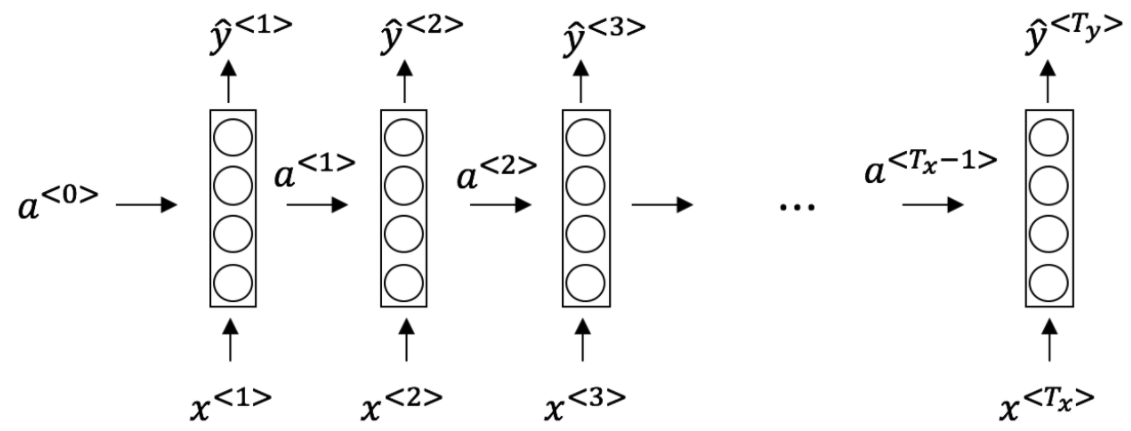
\includegraphics[width=12cm]{RNN.png}
    \caption{Architecture of a basic RNN ($T_x = T_y$)}
    \label{fig:basicRNN}
\end{figure}

\emph{\textcolor{Bittersweet}{One limitation of this particular unidirectional RNN is that the prediction at a certain time uses inputs/information from the inputs earlier in the sequence but not information later in the sequence $\rightarrow$ bi-directional RNN (BRNN).}}\\
\\
\textbf{Forward propagation}
Each cell takes two inputs at each time step: The hidden state from the previous cell; The current time step's input data;\\
Each cell has two outputs at each time step: A hidden state; A prediction.
\begin{align}
a^{\langle t \rangle} &= g_1(w_{aa}a^{\langle t-1 \rangle} + w_{ax}x^{\langle t \rangle} + b_a), \tanh/\text{ReLU}\\
y^{\langle t \rangle} &= g_2(w_{ya}a^{\langle t \rangle} + b_y), \text{Sigmoid}\\
&\rightarrow \nonumber\\
a^{\langle t \rangle} &= g_1(w_{a} [a^{\langle t-1 \rangle}, x^{\langle t \rangle}] + b_a)\\
y^{\langle t \rangle} &= g_2(w_{y}a^{\langle t \rangle} + b_y)\\
& w_a = [w_{aa}; w_{ax}] \nonumber \\
& [a^{\langle t-1 \rangle}, x^{\langle t \rangle}] = \begin{bmatrix}
    a^{\langle t-1 \rangle} \\ x^{\langle t \rangle}
    \end{bmatrix} \nonumber
\end{align}
~\\
\textbf{Backpropagation through time}\\
\begin{figure}[h]
    \centering
    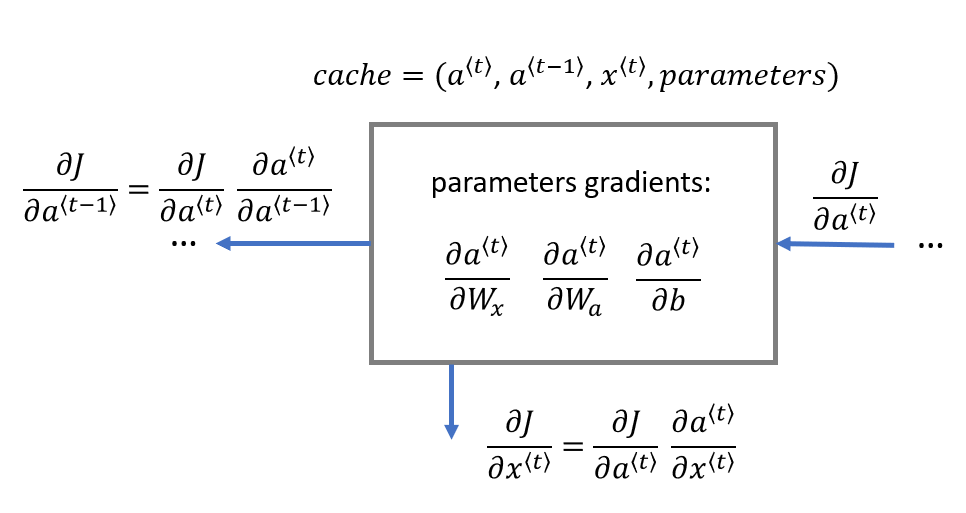
\includegraphics[width=14cm]{rnn_cell_backprop.png}
    \caption{Backpropagation of an RNN cell}
    \label{fig:rnn_cell_backprop}
\end{figure}
Loss function (cross entropy loss):
\begin{align}
L^{\langle t \rangle}(\hat{y}^{\langle t \rangle}, y^{\langle t \rangle}) &= - y^{\langle t \rangle}\log\hat{y}^{\langle t \rangle} - (1-y^{\langle t \rangle})\log(1-\hat{y}^{\langle t \rangle})\\
L(\hat{y}^{\langle t \rangle}, y^{\langle t \rangle}) &= \sum_{t=1}^{T_y} L^{\langle t \rangle}(\hat{y}^{\langle t \rangle}, y^{\langle t \rangle})
\end{align}
In this case, the length of the input sequence was equal to the length of the output sequence (same number of time steps).\\
\begin{align}
\displaystyle a^{\langle t \rangle} &= \tanh(W_{ax} x^{\langle t \rangle} + W_{aa} a^{\langle t-1 \rangle} + b_{a})\\
\displaystyle \frac{\partial \tanh(x)} {\partial x} &= 1 - \tanh^2(x)\\
\displaystyle {dtanh} &= da_{next} * ( 1 - \tanh^2(W_{ax}x^{\langle t \rangle}+W_{aa} a^{\langle t-1 \rangle} + b_{a}))\\
\displaystyle  {dW_{ax}} &= dtanh \cdot x^{\langle t \rangle T}\\
\displaystyle dW_{aa} &= dtanh \cdot a^{\langle t-1 \rangle T}\\
\displaystyle db_a& = \sum_{batch}dtanh\\
\displaystyle dx^{\langle t \rangle} &= { W_{ax}}^T \cdot dtanh\\
\displaystyle da_{prev} &= { W_{aa}}^T \cdot dtanh\\
\end{align}
%%
\subsubsection{Different types of RNNs}
\begin{itemize}
\item
$T_x = T_y$\\
\textit{Many-to-many}\\
Machine translation\\
$T_x \neq T_y$\
\item
Sentiment classification\\
$x = $ text\\
$y = 0 / 1$\\
\textit{Many-to-one}
\item
Music generation\\
$x (x = \phi) \rightarrow y^{\langle 1 \rangle}y^{\langle 2 \rangle} \cdots y^{\langle T_y \rangle}$\\
\textit{One-to-many}
\item
\textit{One-to-one}
\end{itemize}
\begin{figure}[h]
    \centering
    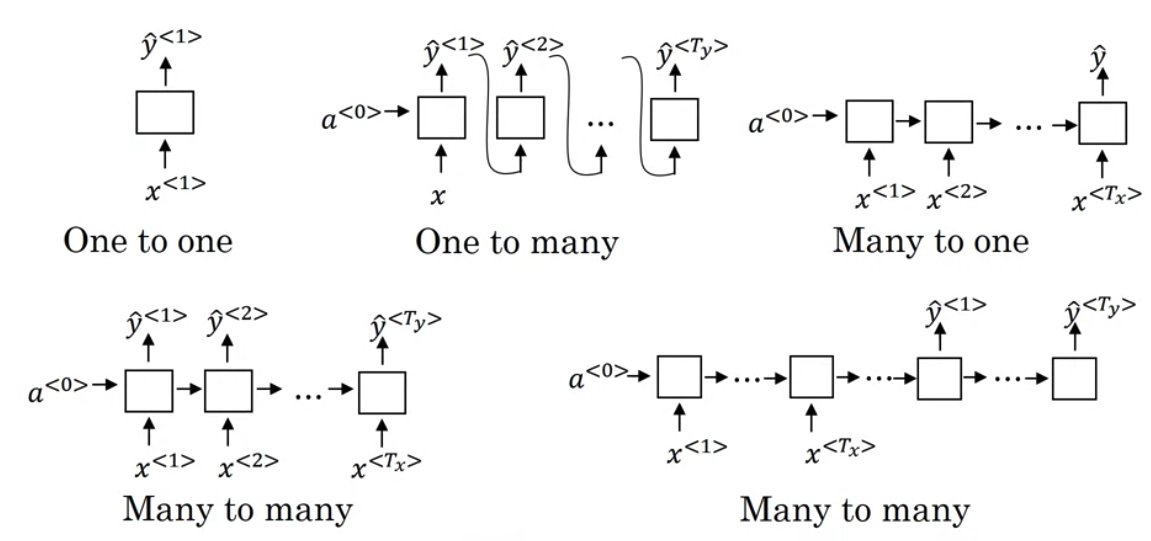
\includegraphics[width=14cm]{differentRNNs.png}
    \caption{Architecture of different RNNs}
    \label{fig:differentRNNs}
\end{figure}

%%
\subsubsection{Language model and sequence generation}
Language model: p(sentence) = ? (output sentences that are likely)\\
Estimate $p(y^{\langle 1 \rangle}y^{\langle 2 \rangle} \cdots y^{\langle T_y \rangle})$\\
\\
Language modelling with an RNN
\begin{itemize}
\item
Training set: large corpus of english text.\\
Tokenize; add <EOS> when a sentence ends; <UNK> for words not in the vocabulary.
\item
Input dummy vecotr of zeros $x^{\langle 1 \rangle} = \overrightarrow{0}, a^{\langle 0 \rangle} = \overrightarrow{0} \rightarrow \hat{y}^{\langle 1 \rangle}$ (length of the vocabulary way Softmax output: the probability of any word in the dictionary)\\
$x^{\langle 2 \rangle} = y^{\langle 1 \rangle}, a^{\langle 1 \rangle} \rightarrow p(\text{current word}|\text{proceeding words}) \cdots$. Run one step of forward propagation to get the first character and the probability distribution for the following character.
\item
Sampling a sequence from a trained RNN\\
Randomly sample a word according to $ \hat{y}^{\langle 1 \rangle}$, pass it into the second and sample according to $ \hat{y}^{\langle 2 \rangle}$ given the procceding word (reject <UNK>), $\cdots$.
\end{itemize}
Character-level language model\\
$y^{\langle 1 \rangle}y^{\langle 2 \rangle} \cdots y^{\langle T_y \rangle}$ would be the individual character.\\
Pros: no unknown words tokens.\\
Cons: end up with much longer sentences.\\

%%
\subsubsection{Vanishing gradients with RNNs}
Gradient vanishing (gradients decrease exponentially): The basic RNN has only ``local'' influence (information that is close to the prediction's time step $t$), not to be good at capturing long-range dependencies.\\
Gradient exploding problem (gradients increase exponentially): Gradient clipping.\\


%
\subsection{Gated recurrent unit (GRU)}
\textit{Cho et al., 2014. On the properties of neural machine translation: Encoder-decoder approaches}\\
\textit{Chung et al., 2014. Empirical Evaluation of Gated Recurrent Neural Networks on Sequence Modeling}\\
\\
$c^{\langle t \rangle} = a^{\langle t \rangle}$ = memory cell
\begin{align}
\tilde{c}^{\langle t \rangle} &= \tanh(w_c[c^{\langle t-1 \rangle}, x^{\langle t \rangle} ] + b_c)\\
\Gamma_u &= \sigma (w_u[c^{\langle t-1 \rangle}, x^{\langle t \rangle}] + b_u), \approx \{0, 1\}, u - \text{update}\\
c^{\langle t \rangle} &= \Gamma_u * \tilde{c}^{\langle t \rangle} + (1- \Gamma_u) * c^{\langle t-1 \rangle}
\end{align}
Full GRU
\begin{align}
\tilde{c}^{\langle t \rangle} &= \tanh(w_c[\Gamma_r * c^{\langle t-1 \rangle}, x^{\langle t \rangle} ] + b_c)\\
\Gamma_u &= \sigma (w_u[c^{\langle t-1 \rangle}, x^{\langle t \rangle}] + b_u)\\
\Gamma_r &= \sigma (w_r[c^{\langle t-1 \rangle}, x^{\langle t \rangle}] + b_r)\\
c^{\langle t \rangle} &= \Gamma_u * \tilde{c}^{\langle t \rangle} + (1- \Gamma_u) * c^{\langle t-1 \rangle}\\
a^{\langle t \rangle} &= c^{\langle t \rangle} 
\end{align}

%
\subsection{Long short term memory (LSTM)}
\begin{figure}[h]
    \centering
    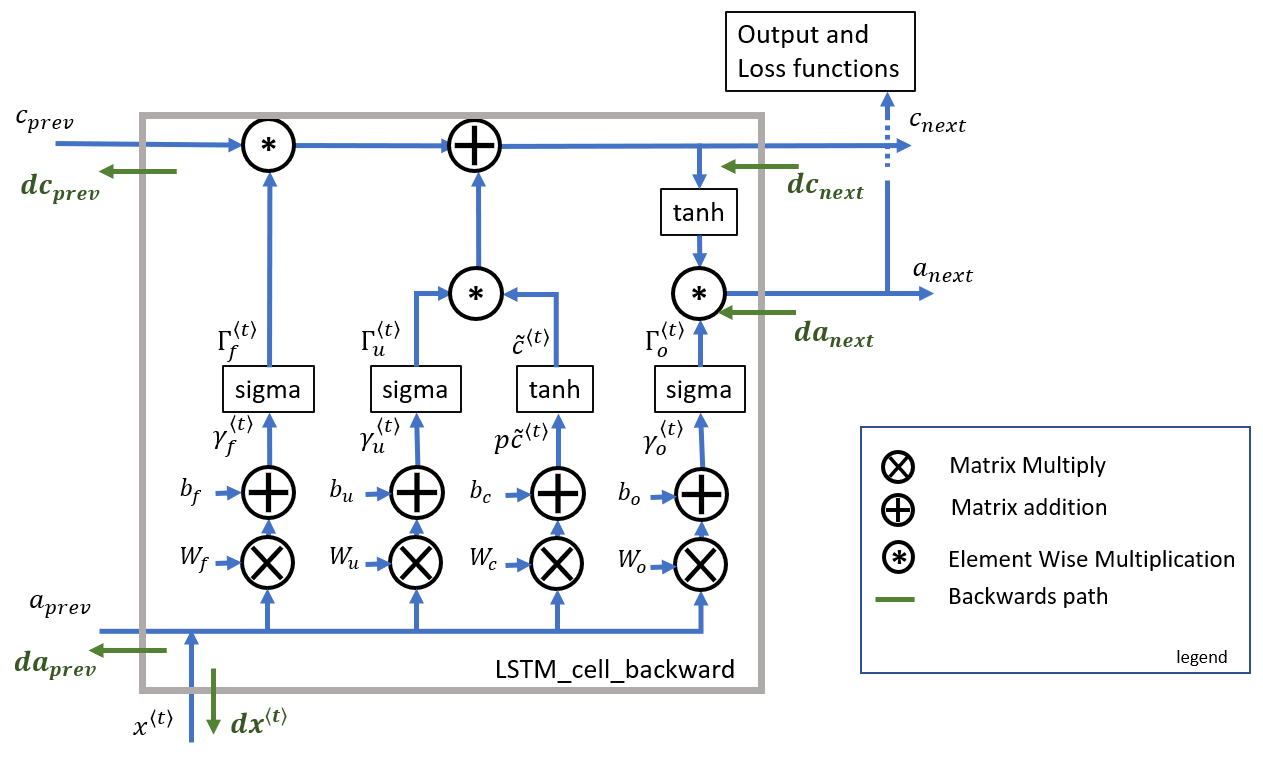
\includegraphics[width=16cm]{LSTM.png}
    \caption{LSTM cell}
    \label{fig:LSTM}
\end{figure}
\textit{Hochreiter \& Schmidhuber 1997. Long short-term memory}
\begin{align}
\tilde{c}^{\langle t \rangle} &= \tanh(w_c[a^{\langle t-1 \rangle}, x^{\langle t \rangle} ] + b_c)\\
\Gamma_u &= \sigma (w_u[a^{\langle t-1 \rangle}, x^{\langle t \rangle}] + b_u), \text{update gate}, \approx {0,1}\\
\Gamma_f  &= \sigma (w_f[a^{\langle t-1 \rangle}, x^{\langle t \rangle}] + b_f), \text{forget gate}, \approx {0,1}\\
\Gamma_o &= \sigma (w_o[a^{\langle t-1 \rangle}, x^{\langle t \rangle}] + b_o), \text{output gate}, \approx {0,1}\\
c^{\langle t \rangle} &= \Gamma_u * \tilde{c}^{\langle t \rangle} + \Gamma_f * c^{\langle t-1 \rangle}\\
a^{\langle t \rangle} &= \Gamma_o * \tanh(c^{\langle t \rangle}) \\
\hat{y}^{\langle t \rangle} &= \text{softmax}(w_{y}a^{\langle t \rangle} + b_y)
\end{align}

Multiplying the gates with the states element-wise (e.g., $Gamma_f* c^{\langle t-1 \rangle}$) is like applying a mask over the cell state.\\
\\
An LSTM is similar to an RNN in that they both use hidden states to pass along information, but an LSTM also uses a cell state, which is like a long-term memory, to help deal with the issue of vanishing gradients. An LSTM cell consists of a cell state, or long-term memory, a hidden state, or short-term memory, along with 3 gates that constantly update the relevancy of its inputs.\\
\\
LSTM as well as the GRU is very good at memorizing certain values, even for a long time for certain real values stored in the memory cells even for many, many times steps.\\
Peephole connection: add $c^{\langle t-1 \rangle}$ to each gate.

%%
\subsubsection{LSTM Backward Pass}
Gate derivatives
\begin{align}
d\gamma_o^{\langle t \rangle} &= da_{next}*\tanh(c_{next}) * \Gamma_o^{\langle t \rangle}*\left(1-\Gamma_o^{\langle t \rangle}\right)\\
dp\widetilde{c}^{\langle t \rangle} &= \left(dc_{next}*\Gamma_u^{\langle t \rangle}+ \Gamma_o^{\langle t \rangle}* (1-\tanh^2(c_{next})) * \Gamma_u^{\langle t \rangle} * da_{next} \right) * \left(1-\left(\widetilde c^{\langle t \rangle}\right)^2\right)\\
d\gamma_u^{\langle t \rangle} &= \left(dc_{next}*\widetilde{c}^{\langle t \rangle} + \Gamma_o^{\langle t \rangle}* (1-\tanh^2(c_{next})) * \widetilde{c}^{\langle t \rangle} * da_{next}\right)*\Gamma_u^{\langle t \rangle}*\left(1-\Gamma_u^{\langle t \rangle}\right)\\
d\gamma_f^{\langle t \rangle} &= \left(dc_{next}* c_{prev} + \Gamma_o^{\langle t \rangle} * (1-\tanh^2(c_{next})) * c_{prev} * da_{next}\right)*\Gamma_f^{\langle t \rangle}*\left(1-\Gamma_f^{\langle t \rangle}\right)
\end{align}
\begin{align}
dW_f &= d\gamma_f^{\langle t \rangle} \begin{bmatrix} a_{prev} \\ x_t\end{bmatrix}^T \\
dW_u &= d\gamma_u^{\langle t \rangle} \begin{bmatrix} a_{prev} \\ x_t\end{bmatrix}^T\\
dW_c &= dp\widetilde c^{\langle t \rangle} \begin{bmatrix} a_{prev} \\ x_t\end{bmatrix}^T\\
dW_o &= d\gamma_o^{\langle t \rangle} \begin{bmatrix} a_{prev} \\ x_t\end{bmatrix}^T
\end{align}
\begin{align}
db_f &= \sum_{batch}d\gamma_f^{\langle t \rangle}\\
db_u &= \sum_{batch}d\gamma_u^{\langle t \rangle}\\
db_c &= \sum_{batch}d\gamma_c^{\langle t \rangle}\\
db_o &= \sum_{batch}d\gamma_o^{\langle t \rangle}
\end{align}
\begin{align}
da_{prev} &= W_f^T d\gamma_f^{\langle t \rangle} + W_u^T   d\gamma_u^{\langle t \rangle}+ W_c^T dp\widetilde c^{\langle t \rangle} + W_o^T d\gamma_o^{\langle t \rangle}\\
dc_{prev} &= dc_{next}*\Gamma_f^{\langle t \rangle} + \Gamma_o^{\langle t \rangle} * (1- \tanh^2(c_{next}))*\Gamma_f^{\langle t \rangle}*da_{next}\\
dx^{\langle t \rangle} &= W_f^T d\gamma_f^{\langle t \rangle} + W_u^T  d\gamma_u^{\langle t \rangle}+ W_c^T dp\widetilde c^{\langle t \rangle} + W_o^T d\gamma_o^{\langle t \rangle}
\end{align}

%
\subsection{Bidirectional RNN}
At the point in time to take information from both earlier and later in the sequence.
\begin{figure}[h]
    \centering
    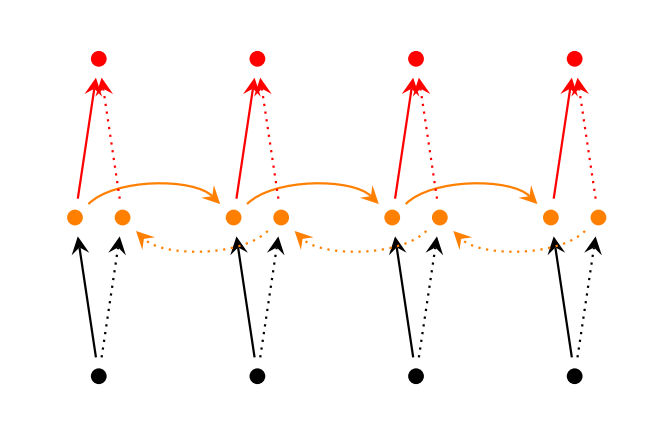
\includegraphics[width=8cm]{bidirectionalrnn.png}
    \caption{Bidirectional-RNN}
    \label{fig:bidirectionalRNN}
\end{figure}
Acyclic graph\\
\begin{align}
\hat{y}^{\langle t \rangle} = g(w_y[\overrightarrow{a}^{\langle t \rangle}, \overleftarrow{a}^{\langle t \rangle}] + b_y)
\end{align}
BRNN with LSTM

%
\subsection{deep RNN}
LSTM has a flag called ``return sequences'' to decide if you would like to return every hidden states or only the last one.
You can use Dropout right after LSTM to regularize your network.
\begin{align}
a^{[l]\langle t \rangle} &= g(w_{a}^{[l]} [a^{[l]\langle t-1 \rangle}, a^{[l-1]\langle t \rangle}] + b_a^{[l]})
\end{align}
\begin{figure}[h]
    \centering
    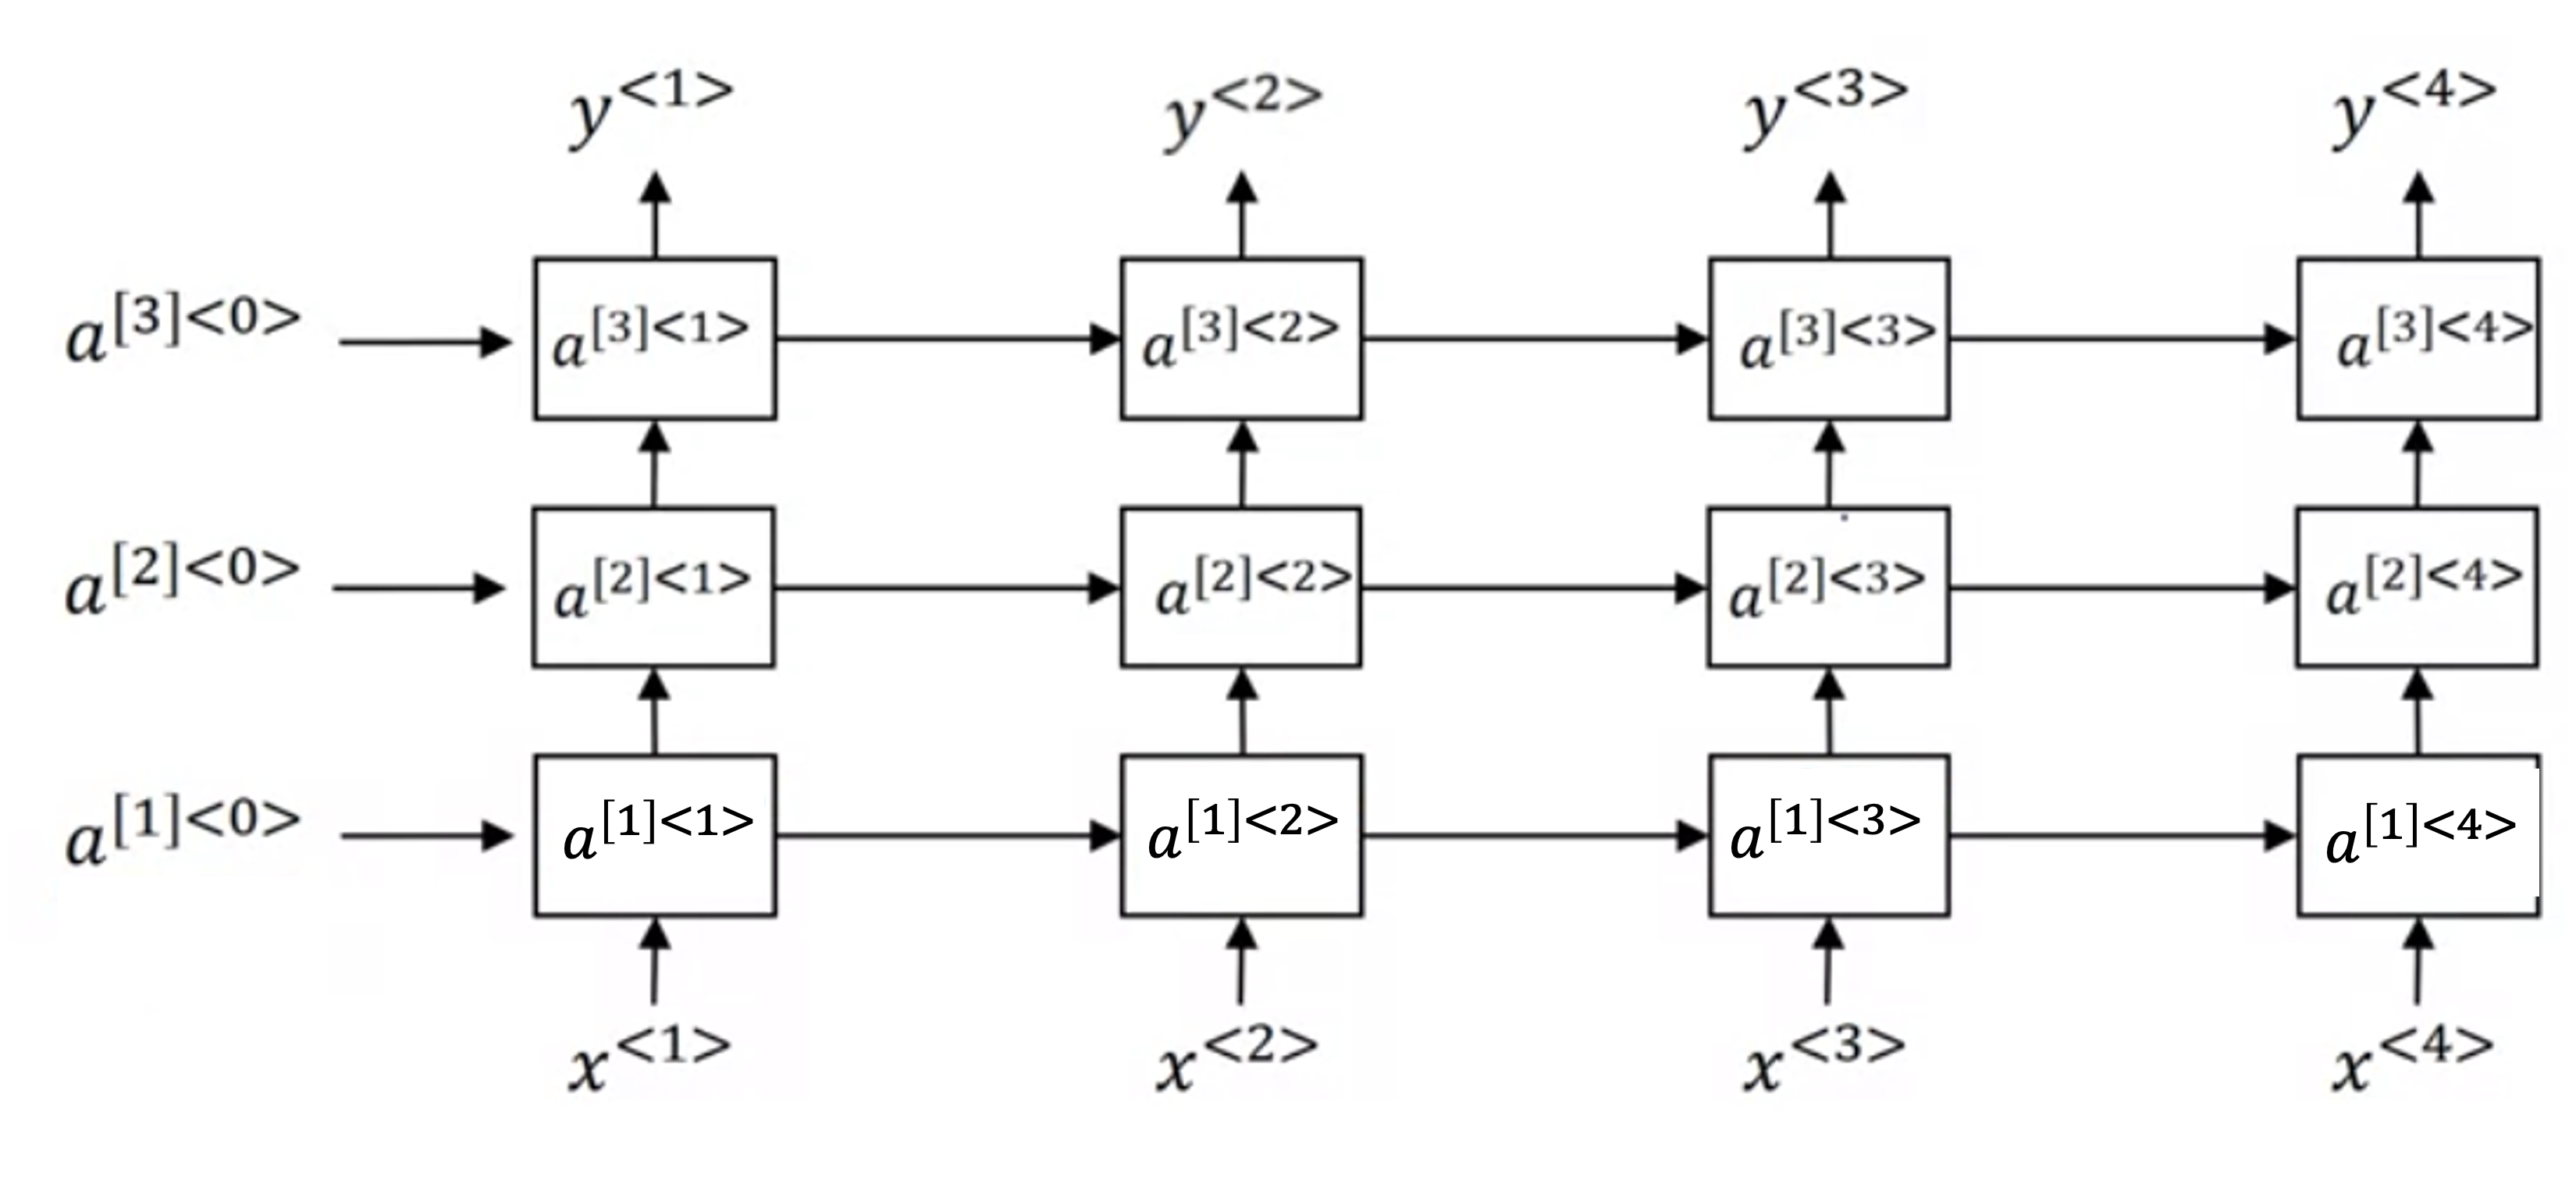
\includegraphics[width=12cm]{deepRNN.png}
    \caption{An deep RNN example}
    \label{fig:deepRNN}
\end{figure}


%_________________________________________________________________
\section{Natural Language Processing \& Word Embeddings}

%
\subsection{Word representation}
V = [a, aaron, ..., zulu, <UNK>]\\
1-hot representation\\
e.g., $O_{5391} = \begin{bmatrix}
0\\0\\0\\0\\ \vdots \\0\\0
\end{bmatrix}$\\
Such 1-hot representation doesn't allow the algorithm to easily generalize across words, because the product between any two different 1-hot vectors is 0.\\
\\
\textbf{Featurized representations}: word embedding. Instead of a 1-hot presentation, to learn a featurized representation with each of the word, e.g., $e_{5391}$. This allows generalize much better across words, though the exact representations are harder to interpret.\\
\\
\textbf{embedding}, visualizing word embeddings (i.e., featurized representations).\\
\textit{van der Maaten and Hinton., 2008. Visualizing data using t-SNE}, non-linear mapping\\
\\
Transfer learning and word embeddings
\begin{enumerate}
\item
Learn word embeddings from large text corpus. (1-100B words), or down load pre-trained embedding online, e.g., pre-trained 50-dimensional GloVe embeddings.
\item
Transfer embedding to new task with smaller training set, e.g., 100k words.
\item
Optional: Continue to finetune the word embeddings with new data.
\end{enumerate}
~\\
Relation to face encoding\\
learn a fixed embedding for each of the word in the fixed vocabulary.\\
\\
Properties of word embeddings\\
\underline{Example}: Analogies\\
\textit{Mikolov et. al., 2013, Linguistic regularities in continuous space word representations}\\
\\
$\displaystyle e_{\text{man}} - e_{\text{woman}} \approx e_{\text{king}} - e_{\text{w}}$\\
Find word $\displaystyle w: \underset{w}{\mathrm{argmin}} ~ \text{similarity}(e_w, e_{\text{king}} - e_{\text{man}} + e_{\text{woman}})$\\
\\
\textbf{Cosine similarity}\\
The cosine of the angle between two vectors is a measure of their similarity.
\begin{align}
\text{CosineSimilarity(u, v)} = \frac {u \cdot v} {||u||_2 ||v||_2} = cos(\theta)
\end{align}
\begin{itemize}
\item
    $u \cdot v$ is the dot product (or inner product) of two vectors
\item
    $||u||_2$ is the norm (or length) of the vector, $ ||u||_2 = \sqrt{\sum_{i=1}^{n} u_i^2}$.
\item
    $\theta$ is the angle between $u$ and $v$. 
\item
    The cosine similarity depends on the angle between $u$ and $v$. 
    \begin{itemize}
    \item
    If $u$ and $v$ are very similar, their cosine similarity will be close to 1.
    \item
     If they are dissimilar, the cosine similarity will take a smaller value.
    \end{itemize}
\end{itemize}

\emph{\textcolor{Bittersweet}{Cosine similarity is a good way to compare the similarity between pairs of word vectors. Note that L2 (Euclidean) distance also works. For NLP applications, using a pre-trained set of word vectors is often a great way to get started.}}
    
%
\subsection{Learning word embeddings}
\subsubsection{Word2Vec}
Embedding matrix E: $E \cdot O_{6257}= e_{6257}$\\
In practice, use specialized function to look up an embedding.\\
\textit{Bengio et. al., 2003, A neural probabilistic language model}\\
Context/target pairs\\
Context:
\begin{itemize}
\item
Natural language model: Last 4 words.
\item
Word embedding: 4 words on left \& right; Last 1 word.
\end{itemize}

An embedding layer can be initialized with pretrained embedding matrix.
%%
\subsubsection{Skip-grams}
\textit{Mikolov et. al., 2013. Efficient estimation of word representations in vector space.}\\
\\
Vocab size = 10,000\\
500-dimensional word embeddings\\
Mapping: Context c (``orange'') $\rightarrow$ Target t (``juice'')
\begin{align}
O_c \rightarrow E \rightarrow e_c \rightarrow \text{softmax unit} \rightarrow \hat{y}
\end{align}
Softmax: $\displaystyle p(t|c) = \frac{e^{\theta_t^T e_c}}{\sum_{j=1}^{10,000}e^{\theta_j^T e_c}}$\\
$\displaystyle \theta_t = $ parameter associated with output $t$\\
$\theta_t$ and $e_c$ are both 500 dimensional vectors (initialized randomly at the beginning of training), trained with an optimization algorithm such as Adam or gradient descent. It is okay if the algorithm does poorly on this artificial prediction task; the more important by-product of this task is a useful set of word embeddings.\\
$\displaystyle L(\hat{y}, y) = - \sum_{j=1}^{10,000}y_i \log \hat{y}_i$\\
$y = \begin{bmatrix}
0\\ \vdots \\ 1 \\ 0 \\ \vdots \\ 0
\end{bmatrix}$ is the 1-hot representation of the target.\\
Computation cost (the softmax part is very computationally heavy) $\rightarrow$ Hierarchical softmax\\
\\
How to sample the context $c$?\\
Uniformly random $\rightarrow$ the, of, a, and, to, etc.\\
Balance out sampling with respect to $p(c)$.

%%
\subsubsection{Negative sampling}
\textit{Mikolov et. al., 2013. Distributed representation of words and phrases and their compositionality}\\
Defining a new learning problem\\
\begin{center}
\begin{tabular}{ m{2cm} m{2cm} m{2cm}}
Context & Word & Target\\
c & t & y\\
\hline
orange & juice & 1\\
orange & king  & 0\\
orange & book & 0\\
orange & the    & 0\\
orange & of      & 0\\
\end{tabular}
\end{center}
One positive example and $k$ randomly selected negative examples.
$\displaystyle p(y = 1 | c, t) = \sigma (\theta_t^T e_c)$
10,000-way softmax $\rightarrow$ 10,000 binary logistic classification problems, on every iteration only train k+1 of them (k negative examples).\\
\\
Selecting negative examples\\
Heuristic $\displaystyle p(w_i) = \frac{f(w_i)^{3/4}}{\sum_{j = 1}^{10,000} f(w_j)^{3/4}}$, which is proportional to the empirical frequency $f(w_i)$.

%%
\subsubsection{GloVe word vectors}
\textit{Pennington et. al., 2014. GloVe: Global vectors for word representation}\\
$x_{ij} = $ \# times ~ $j (t)$ ~ appears in context of ~ $i(c)$.
\begin{align}
\displaystyle \min \sum_{i =1}^{10,000} \sum_{j =1}^{10,000} f(x_{ij})(\theta_i^T e_j + b_i + b'_j- \log x_{ij})^2
\end{align}
weighting term:
\begin{equation*}
f(x_{ij})  = \left\{ 
    \begin{array}{l}
    0 ~ \text{if} ~ x_{ij} = 0\\
    \text{heuristics for (in)frequent words}
    \end{array} \right.
\end{equation*}

\emph{\textcolor{Bittersweet}{$\displaystyle \theta_i^T e_j = (A\theta_i)^T(A^{-T}\theta_i)$. The individual components of the embeddings might not be interpretable. The axis used to represent the features might not be aligned with that night be easily humanly interpretable axis (potentially arbitrary linear transformation of the features).}}

%
\subsection{Sentiment classification}
Sentiment classification problem\\
x (a piece of texts) $\longrightarrow$ y (positive, negative, e.g., stars)
\begin{figure}[h]
\centering
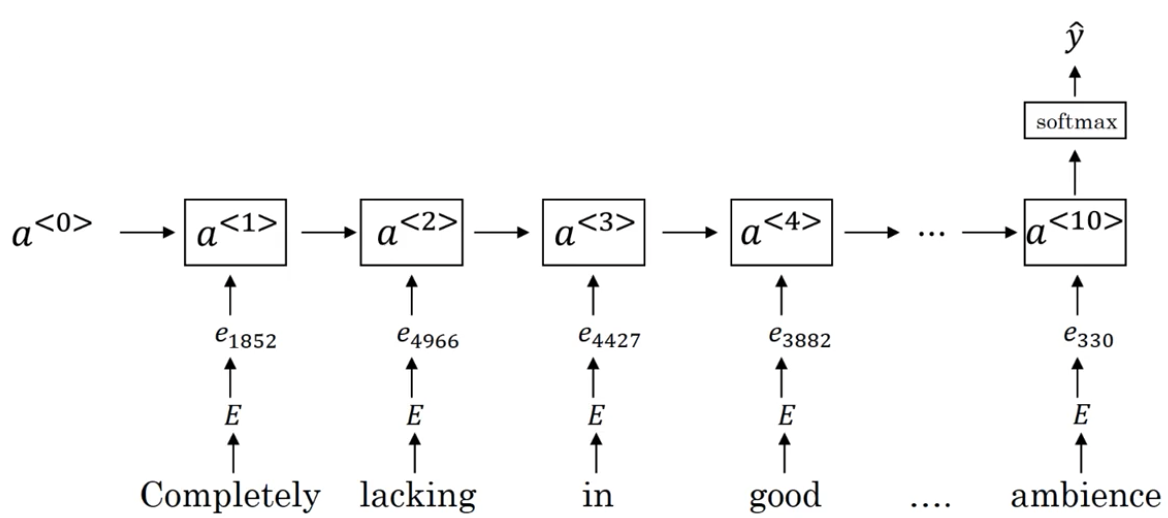
\includegraphics[width=12cm]{RNNsentiment.png}
\caption{RNN for sentiment classification}
\label{fig:RNNsentiment}
\end{figure}

%
\subsection{Debiasing word embeddings}
The problem of bias in word embeddings\\
\textit{Bolukbasi et. al., 2016. Man is to computer programmer as woman is to homemaker? Debiasing word embedding}\\
Word embeddings can reflect gender, ethnicity, age, sexual, orientation, and other biases of the text used to train the model.\\
Addressing bias in word embeddings
\begin{enumerate}
\item
Identify bias direction.
\item
Neutralize: For every word that is not definitional, project to get rid fo bias.\\
$$e^{bias\_component} = \frac{e \cdot g}{||g||_2^2} * g$$
$$e^{debiased} = e - e^{bias\_component}$$
$e^{bias\_component}$ as the projection of $e$ onto the direction $g$.
\item
Equalize pairs.
\end{enumerate}


%_________________________________________________________________
\section{Sequence to sequence models}
\begin{itemize}
\item
Machine translation\\
\textit{Sutskever et al., 2014. Sequence to sequence learning with neural networks}\\
\textit{Cho et al., 2014. Learning phrase representations using RNN encoder-decoder for statistical machine translation}
\item
Image caption\\
\textit{Mao et. al., 2014. Deep captioning with multimodal recurrent neural networks}\\
\textit{Vinyals et. al., 2014. Show and tell: Neural image caption generator}\\
\textit{Karpathy and Li, 2015. Deep visual-semantic alignments for generating image descriptions}
\end{itemize}
\begin{figure}[h]
    \centering
    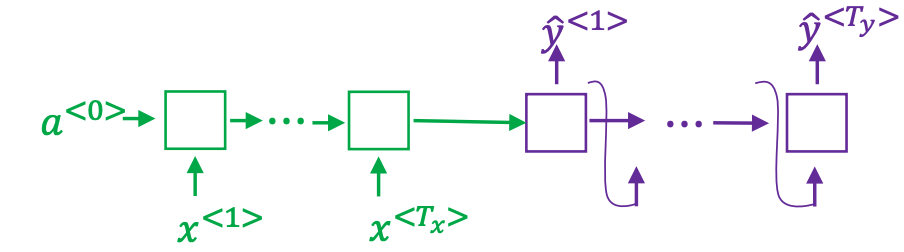
\includegraphics[width=12cm]{machinetranslation.png}
    \caption{Machine translation, where $T_x$ and $T_y$ an be different.}
    \label{fig:machinetranslation}
\end{figure}
~\\
Machine translation as building a conditional language model
\begin{itemize}
\item
Language model: $\displaystyle p(y^{\langle1\rangle}, \cdots, y^{\langle T_y \rangle})$
\item
    Machine translation: encoder $\rightarrow$ Language model
    \begin{itemize}
    \item
    ``Conditional language model'', $\displaystyle p(y^{\langle 1 \rangle}, \cdots, y^{\langle T_y\rangle} | x^{\langle 1 \rangle}, \cdots, x^{\langle T_x \rangle})$
    \item
    Pick the most likely sentence (translation):\\
    $\displaystyle \underset{y^{\langle 1 \rangle}, \cdots, y^{\langle T_y\rangle}}{\mathrm{argmin}} p(y^{\langle 1 \rangle}, \cdots, y^{\langle T_y\rangle} | x^{\langle 1 \rangle}, \cdots, x^{\langle T_x \rangle})$
    \end{itemize}
\end{itemize}

%
\subsection{Beam search algorithm}
For instance, beam width B = 3, three copies of the network to evaluate the partial sentence fragments and the output are instantiated.
\begin{itemize}
\item
Step 1: $\displaystyle  p(y^{\langle 1 \rangle} | x) \rightarrow \hat{y}^{\langle 1 \rangle}$
\item
Step 2: $\displaystyle  p(y^{\langle 1 \rangle}, y^{\langle 2 \rangle} | x) = p(\hat{y}^{\langle 1 \rangle} | x) p(\hat{y}^{\langle 2 \rangle} | x, \hat{y}^{\langle 1 \rangle})  \rightarrow \hat{y}^{\langle 2 \rangle}$
\item
Step 3: $\displaystyle  p(y^{\langle 3 \rangle}| x, \hat{y}^{\langle 1 \rangle}  , \hat{y}^{\langle 2 \rangle} )  \rightarrow \hat{y}^{\langle 3 \rangle}$
\item
$\cdots$
\end{itemize}
B=1: greedy search

%%
\subsubsection{Length normalization}

\begin{align*}
&\underset{y}{\mathrm{argmin}} \prod_{t=1}^{T_y} p(y^{\langle t \rangle} | x, y^{\langle 1 \rangle}, \cdots, y^{\langle t-1 \rangle}) = \underset{y^{\langle 1 \rangle}, \cdots, y^{\langle T_y\rangle}}{\mathrm{argmin}} p(y^{\langle 1 \rangle}, \cdots, y^{\langle T_y\rangle} | x^{\langle 1 \rangle}, \cdots, x^{\langle T_x \rangle})\\
& \underset{y}{\mathrm{argmin}} \sum_{t=1}^{T_y} \log p(y^{\langle t \rangle} | x, y^{\langle 1 \rangle}, \cdots, y^{\langle t-1 \rangle})\\
& \frac{1}{T_y^{\alpha}}\underset{y}{\mathrm{argmin}} \sum_{t=1}^{T_y} \log p(y^{\langle t \rangle} | x, y^{\langle 1 \rangle}, \cdots, y^{\langle t-1 \rangle})\\
\end{align*}
hyper-parameter $0 \le \alpha \le 1$ for between full and no normalizing by length (hack).\\
\\
How to choose the beam width B?\\
Large B: Better result, slower\\
Small B: Worse result, faster.\\

\emph{\textcolor{Bittersweet}{Unlike exact search algorithms like BFS (Breadth First Search) or DFS (Depth First Search), Beam Search runs faster but is not guaranteed to find exact maximum for $\underset{y}{\mathrm{argmin}} p(y^{\langle t \rangle} | x)$}}

%%
\subsubsection{Error analysis}
To figure out what fraction of errors are due to RNN encoder-decoder vs. beam search\\
\underline{Example}: $y*$ human translation.
\begin{itemize}
\item
Case 1\\
$p(\hat{y}^{\langle t \rangle} | x) \leq p(y^{* \langle t \rangle} | x)$\\
Beam search chose $\hat{y}$, but $y*$ attains higher $p(y | x)$.\\
Conclusion: Beam search is fault.
\item
Case 2\\
$p(\hat{y}^{\langle t \rangle} | x) \geq p(y^{* \langle t \rangle} | x)$\\
$y*$ is a better translation than $\hat{y}$, but RNN predicted $p(\hat{y}^{\langle t \rangle} | x) > p(y^{* \langle t \rangle} | x)$.\\
Conclusion: RNN search is fault.
\end{itemize}


%
\subsection{Bleu score}
Evaluating machine translation\\
\textit{Papineni et. al., 2002. Bleu: A method for automatic evaluation of machine translation}\\
Bleu score on unigrams/bigrams/ngrams\\
$p_n = $ Bleu score on n-grams only
\begin{align}
p_n = \frac{\sum_{\text{n-grams} \in \hat{y}} \text{Count}_{\text{Clip}}(\text{n-gram})} {\sum_{\text{n-grams} \in \hat{y}} {\text{Count}(\text{n-gram})}}
\end{align}
Combined Bleu score: $\displaystyle \text{BP}\exp(\frac{1}{4}\sum_{n=1}^4 p_n)$\\
BP = brevity penalty\\
\begin{equation*}
BP = \left\{ \begin{array}{l} \text{1, ~ if MT output length > reference output length}\\
\text{exp(1- reference output length / MT output length), ~ otherwise} \end{array} \right.
\end{equation*}


%
\subsection{Attention model}
\begin{figure}[h]
    \centering
    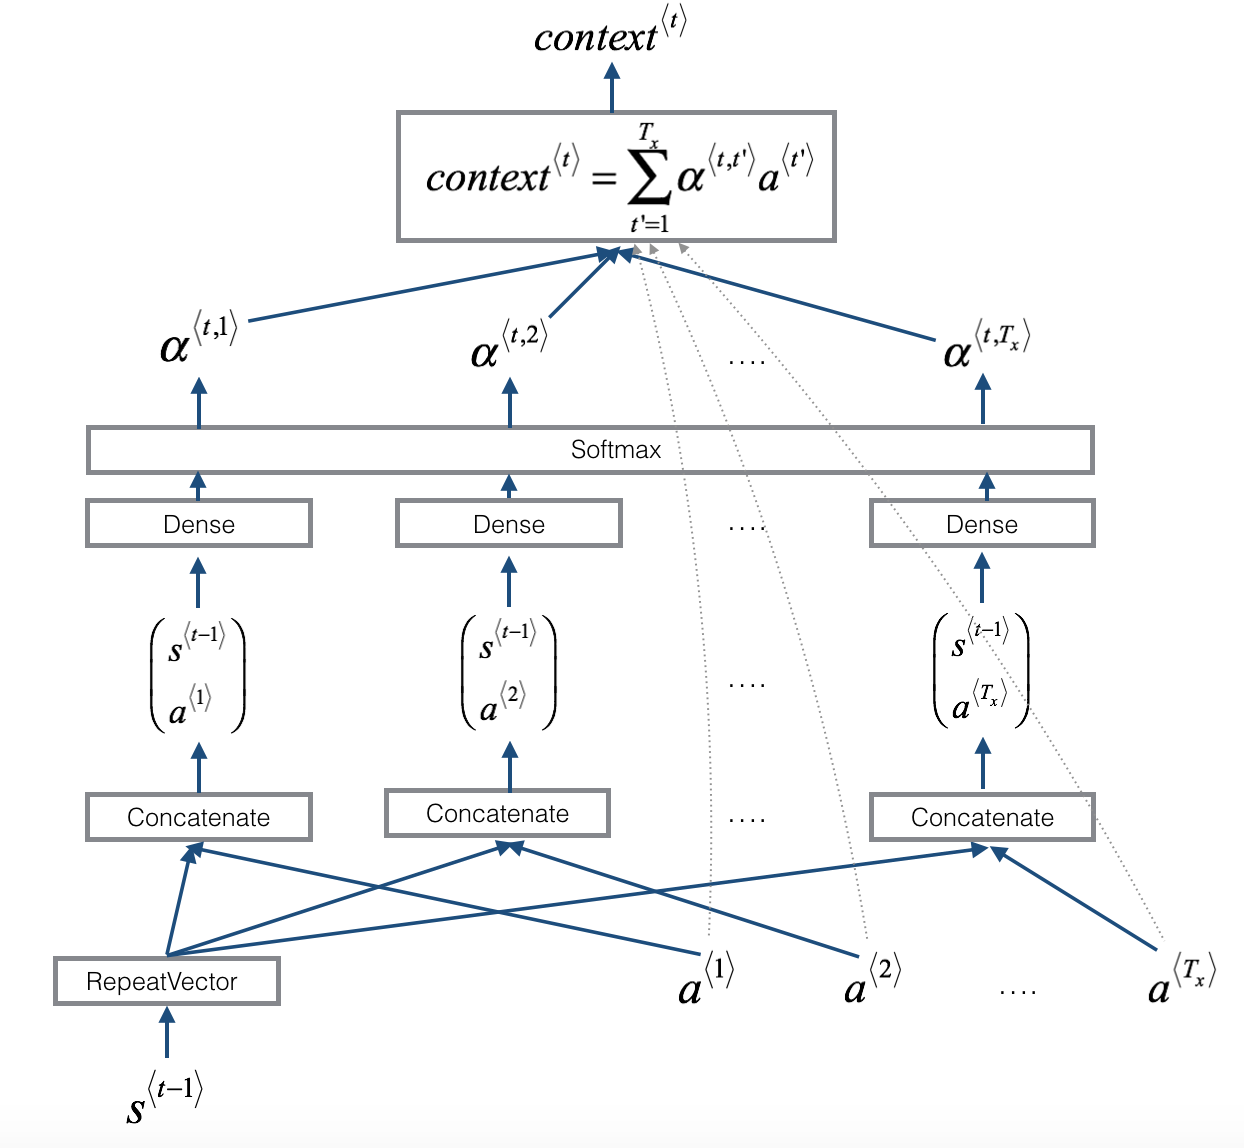
\includegraphics[width=14cm]{attn_mechanism.png}
    \caption{Attention mechanism. RepeatVector node is used to to copy $s^{\langle t \rangle}$'s value $T_x$  times. The concatenation of $s^{\langle t-1 \rangle}$ and $a^{\langle t \rangle}$ is fed into a ``Dense'' layer, which computes $e^{\langle t, t' \rangle}$. $e^{\langle t, t' \rangle}$ is then passed through a softmax to compute $\alpha^{\langle t, t' \rangle}$.}
    \label{fig:Attentionmechanism}
\end{figure}

\textit{Bahdanau et. al., 2014. Neural machine translation by jointly learning to align and translate}\\
\textit{Xu et. al., 2015. Show, attend and tell: Neural image caption generation with visual attention}\\
\\
The attention model allows a neural network to pay attention to only part of an input sentence while it's generating a translation. The attention mechanism tells a Neural Machine Translation model where it should pay attention to at any step.\\
\\
The pre-attention Bi-LSTM goes through $T_x$  time steps. The post-attention LSTM goes through $T_y$  time steps. Note that an LSTM passes both the hidden state $s^{\langle t \rangle}$ and cell state $c^{\langle t \rangle}$ from one time step to the next.
\begin{figure}[h]
    \centering
    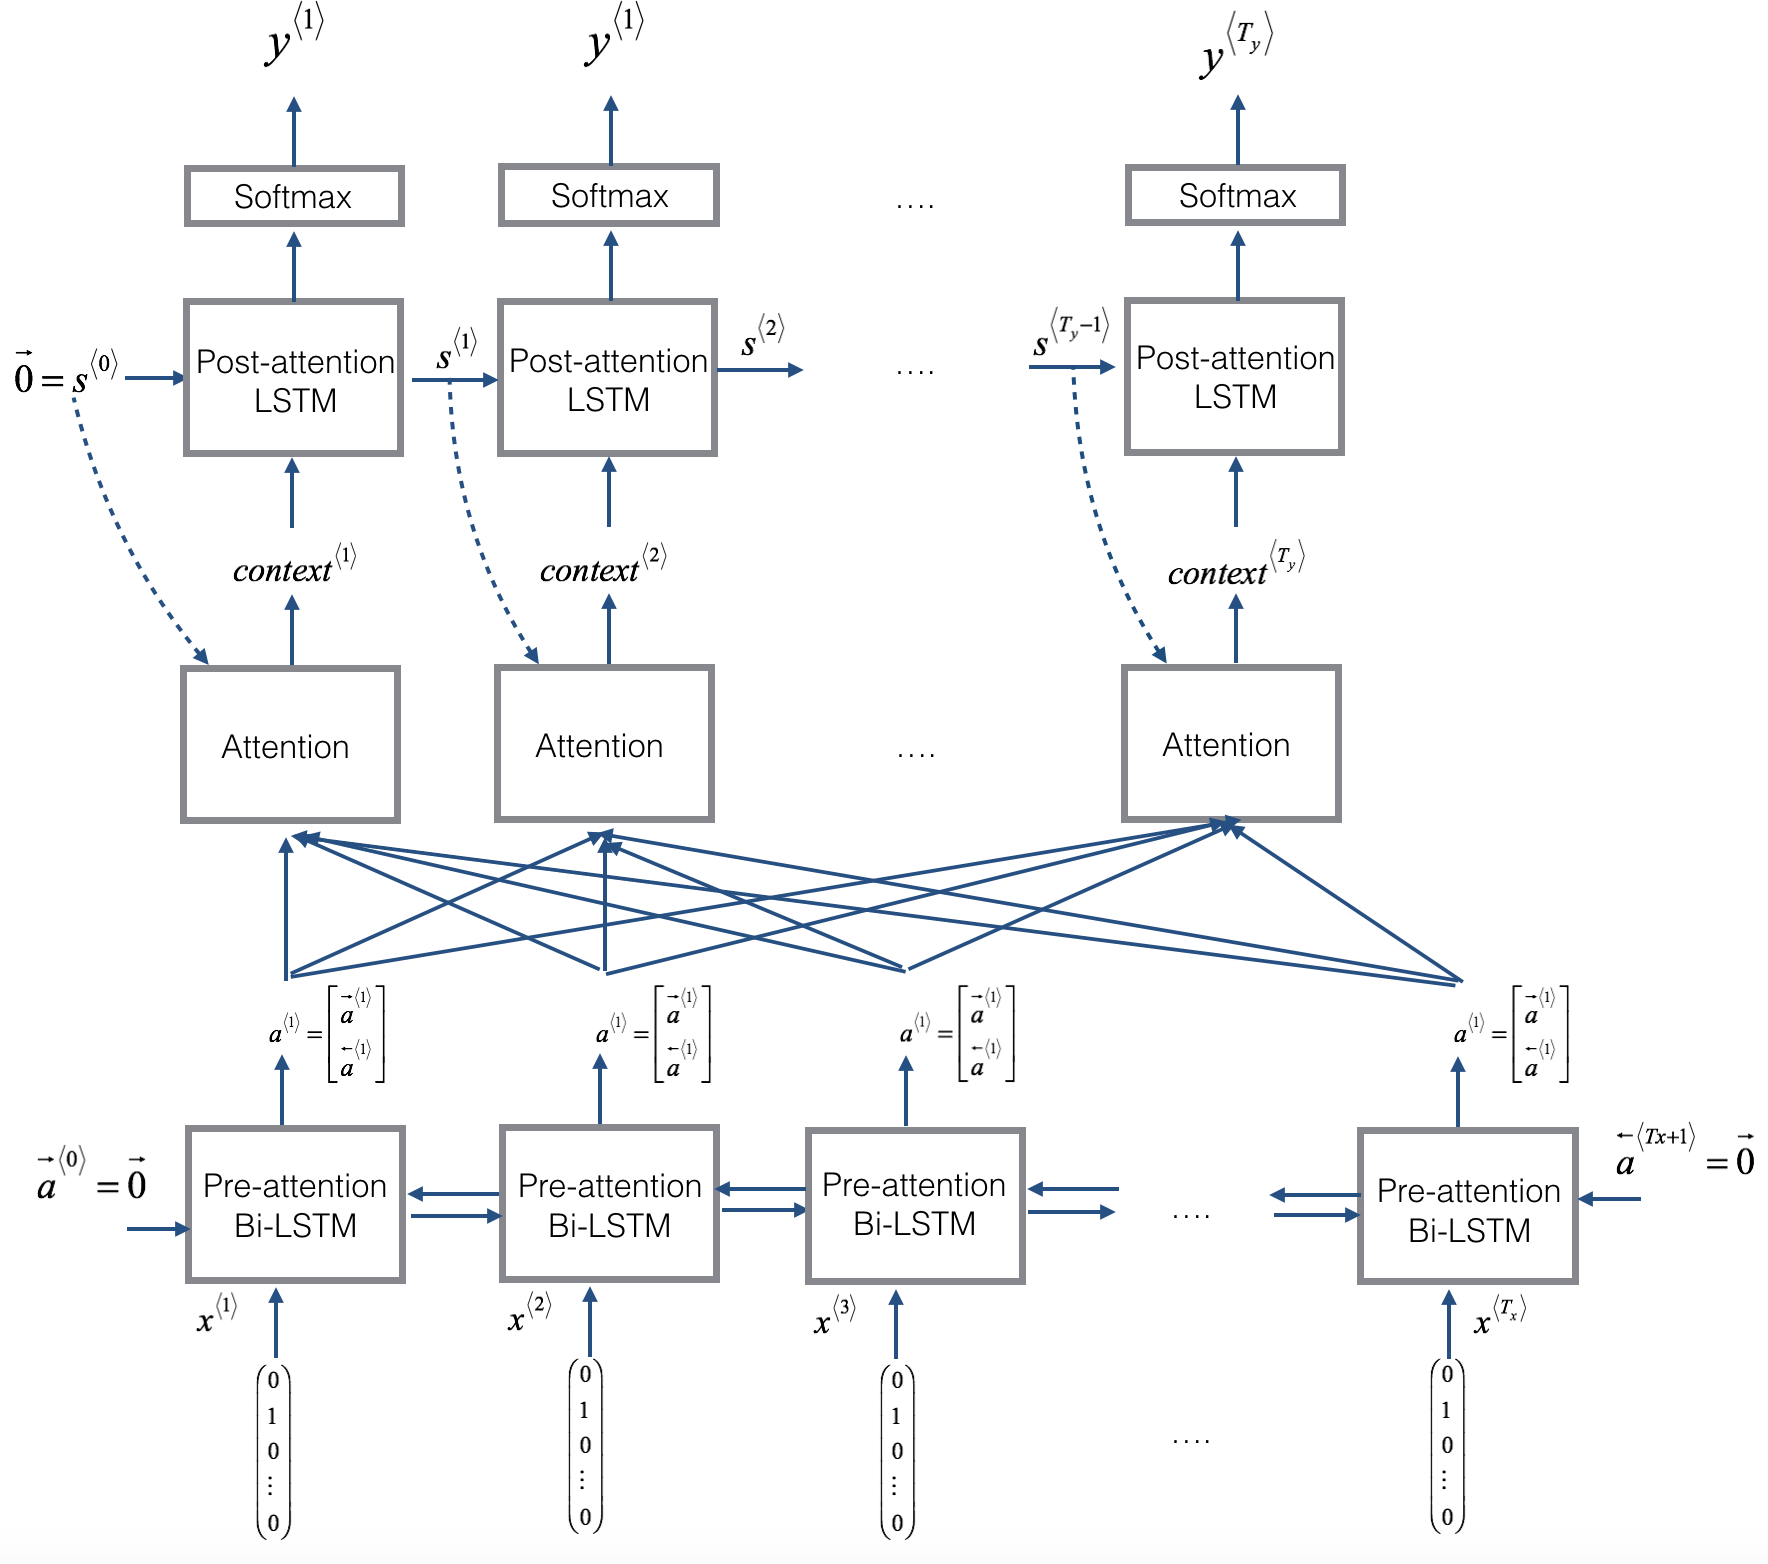
\includegraphics[width=16cm]{attn_model.png}
    \caption{Attention model}
    \label{fig:Attentionmodel}
\end{figure}

\begin{align}
&a^{\langle t' \rangle} = (\overrightarrow{a}^{\langle t' \rangle}, \overleftarrow{a}^{\langle t' \rangle})\\
&\sum_{t'} \alpha^{\langle 1, t' \rangle} = 1\\
&context^{\langle t \rangle } = \sum_{t'} \alpha^{\langle t, t' \rangle} a^{\langle t' \rangle} 
\end{align}
$\alpha^{\langle t, t' \rangle} = $ amount of ``attention'' $y^{\langle t \rangle }$ should pay to $a^{\langle t' \rangle}$\\
\\
Computing attention $\alpha^{\langle t, t' \rangle}$:
\begin{align}
\alpha^{\langle t, t' \rangle} = \frac{\exp{e^{\langle t, t' \rangle}}}{\sum_{t' = 1}^{T_x} \exp{e^{\langle t, t' \rangle}}}
\end{align}
attention weights sum to 1, summation over $t'$.\\
use a small neural network to compute the ``energies'' $e^{\langle t, t' \rangle}$ as a function of $s^{\langle t-1 \rangle}$ and $a^{\langle t' \rangle}$. $s^{\langle t-1 \rangle}$ is the hidden state of the post-attention LSTM. $a^{\langle t' \rangle}$ is the hidden state of the pre-attention LSTM.

\begin{figure}[h]
    \centering
    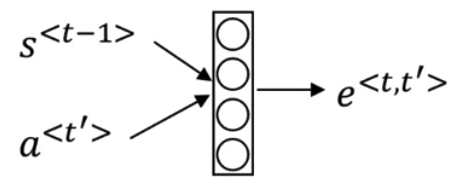
\includegraphics[width=5cm]{ettprime.png}
    \caption{Computing the $e^{\langle t, t' \rangle}$ using a small neural network}
    \label{fig:ettprime}
\end{figure}
~\\
Visualization of $\alpha^{\langle t, t' \rangle}$ as a full attention map, to see what the network is paying attention to while generating each output.\\

%
\subsection{Speech recognition}
x (audio clip) $\longrightarrow$ y (transcript)\\
Attention model for speech recognition\\
CTC cost for speech recognition\\
\textit{Graves et al., 2006. Connectionist Temporal Classification: Labeling unsegmented sequence data with recurrent neural networks}\\
\\
Trigger word detection\\
$x{\langle t \rangle}$ is features of the audio (such as spectrogram features) at time $t$.\\
Using a spectrogram and optionally a 1D CONV layer is a common pre-processing step prior to passing audio data to an RNN, GRU or LSTM.


%_________________________________________________________________
\section{Transformer network}
\textit{Vaswani et al. 2017, Attention Is All You Need}\\
Attention mechanism + CNN style of processing\\
Parallel processing: A Transformer Network can ingest entire sentences all at the same time.

\begin{itemize}
\item
Self-Attention
\item
Multi-Head Attention
\end{itemize}

%%
\subsubsection{Self-attention}

Calculate for each word\\
A(q, k, v) = attention-based vector representation of a word\\
Given a word, its neighbouring words are used to compute its context by summing up the word values to map the Attention related to that given word.
\begin{figure}[h]
    \centering
    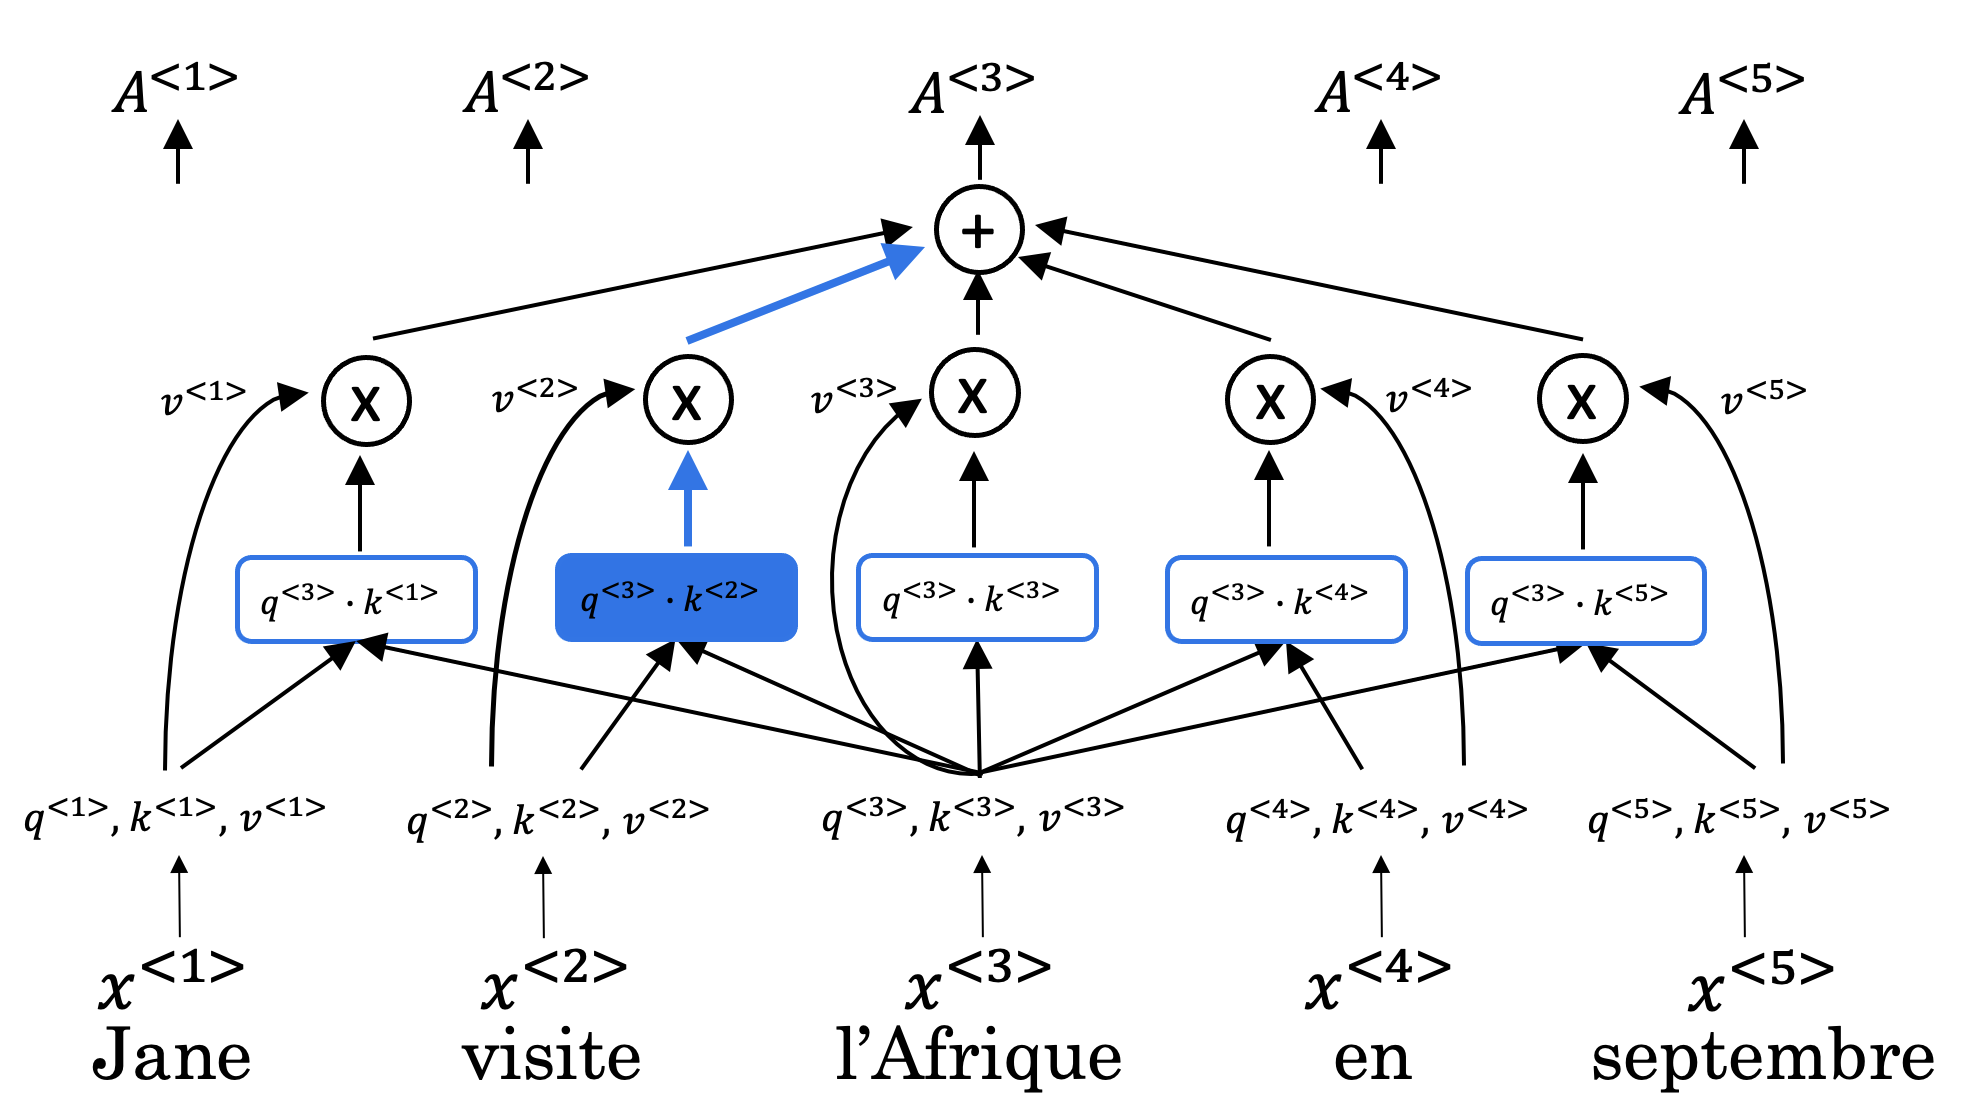
\includegraphics[width=14cm]{selfattention.png}
    \caption{The concept of \textit{Self-Attention}}
    \label{fig:selfattention.}
\end{figure}

\begin{center}
\begin{tabular}{ m{6cm}  m{8cm}  }
RNN Attention & Transformer Attention\\
$\displaystyle \alpha^{\langle t, t' \rangle} = \frac{\exp{e^{\langle t, t' \rangle}}}{\sum_{t' = 1}^{T_x} \exp{e^{\langle t, t' \rangle}}}$ &
$\displaystyle A(q, K, V) = \sum_i \frac{\exp{e^{\langle q \cdot k^{\langle i \rangle \rangle}}}}{\sum_{j}\exp{e^{\langle q \cdot k^{\langle j \rangle \rangle}}}} v^{\langle i \rangle}$\\
\end{tabular}
\end{center}
Q = interesting questions about the words in a sentence\\
K = qualities of words given a Q\\
V = specific representations of words given a Q
\begin{align*}
q^{\langle t \rangle} &= W^Q \cdot x^{\langle t \rangle}\\
k^{\langle t \rangle} &= W^K \cdot x^{\langle t \rangle}\\
v^{\langle t \rangle} &= W^V \cdot x^{\langle t \rangle}\\
\end{align*}

\begin{center}
\begin{tabular}{ m{2cm}  m{2cm}  m{2cm}}
Query (Q) & Key(K) & Value (V)\\
$q^{\langle 1 \rangle}$ & $k^{\langle 1 \rangle}$ & $v^{\langle 1 \rangle}$\\
$q^{\langle 2 \rangle}$ & $k^{\langle 2 \rangle}$ & $v^{\langle 2 \rangle}$\\
$q^{\langle 3 \rangle}$ & $k^{\langle 3 \rangle}$ & $v^{\langle 3 \rangle}$\\
$q^{\langle 4 \rangle}$ & $k^{\langle 4 \rangle}$ & $v^{\langle 4 \rangle}$\\
$q^{\langle 5 \rangle}$ & $k^{\langle 5 \rangle}$ & $v^{\langle 5 \rangle}$\\
\end{tabular}
\end{center}
\begin{align}
Attention(Q, K, V) = softmax(\frac{QK^T}{\sqrt{d_k}})V
\end{align}
$d_k$ is the dimension of the keys, which is used to scale everything down so the softmax doesn't explode.

%%
\subsubsection{Multi-head attention}
``head'': self-attention\\
Doing the self-attention multiple times to learn a much richer, much better representation for every word.
\begin{align*}
head_i &= Attention(W_i^Q Q, W_i^K K, W_i^V V)\\
multiHead(Q, K, V) &= concat(head_i head_2 \cdots head_h)W_o
\end{align*}
$i$ here represents the computed attention weight matrix associated with the $i-th$ “head” (sequence).\\
\\
Transformer\\
$\langle SOS \rangle x^{\langle 1 \rangle} x^{\langle t2\rangle} \cdots x^{\langle T_x -1 \rangle} x^{\langle T_x \rangle} \langle EOS \rangle $
The decoder takes from the Encoder V and K for its second block of Multi-Head Attention, but takes its own cumulative previous predictions Q.

\begin{figure}[h]
    \centering
    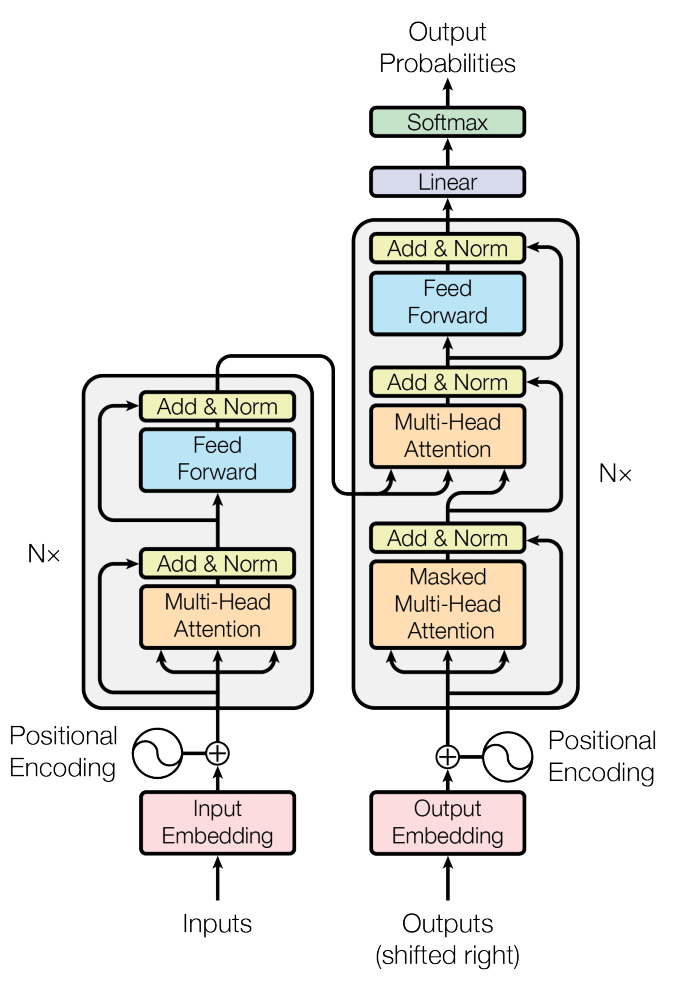
\includegraphics[width=12cm]{transformer.png}
    \caption{The Transformer - model architecture.}
    \label{fig:transformer}
\end{figure}

%%
\subsubsection{Positional encoding}
To encode the positions of the inputs and pass them into the network using sine and cosine formulas:
\begin{align}
PE_{(pos, 2i)} &= \sin\left(\frac{pos}{{10000}^{\frac{2i}{d}}}\right)\\
PE_{(pos, 2i+1)} &= \cos\left(\frac{pos}{{10000}^{\frac{2i}{d}}}\right)
\end{align}
\begin{itemize}
\item
$d$ the dimension of the word embedding and positional encoding.
\item
$pos$ is the position of the word.
\item
$i$ refers to each of the different dimensions of the positional encoding.
\end{itemize}
The sum of the positional encoding and word embedding is ultimately what is fed into the model. The values of the sine and cosine equations are small enough (between -1 and 1) that when you add the positional encoding to a word embedding, the word embedding is not significantly distorted, and is instead enriched with positional information.

\end{document}